% !TEX program = lualatex
% MHM2010 / T4 Maser Timing Workbench documentation
% Version: 0.3.0 | Author: William W. Wallace | Created: 2026-11-03 | Modified: 2026-11-11
% Revision: 0.1.0 Initial operator manual, validation and equation appendix.
%           0.2.0 T4 iMaser 3000, reference 1 PPS figures, MJD/local time axes.
%           0.2.1 T4 monitoring files (FTP ./Monitoring), operator reboot
%                 script, local UDP port 14000, REBOOT wording and page cites.
%           0.2.2 View > Time display (MJD / ISO 8601 local / UTC), fit
%                 windows (last 30 and 90 days), where the Veusz files are.
%           0.2.3 Suggested settings: frequency AND drift (MHM2010 DDS counts,
%                 drift in pp18/day and DDS counts/day; T4 SETFSREL and
%                 DRIFTCOMP) in the figure, Results and exports; exports
%                 with exact numbers, meaningful names and Veusz tags.
%           0.2.4 Writer 0.0.29 (master 0.0.28 + exact ISO 8601 text);
%                 times as text with every digit; T4 recorder CSVs exact.
%           0.3.0 Further evaluation tabs (gap-aware stability with
%                 confidence intervals, steering removal, Kalman estimate,
%                 three-cornered hat); Veusz page checkboxes and batch flags;
%                 manual reorganized by topic; a variable table before every
%                 equation block; Appendix B (all variables) and Appendix C
%                 (all stability traces); lists of tables and figures in the
%                 contents and the PDF bookmarks.
% Build three times: lualatex -interaction=nonstopmode -halt-on-error <this file>
\documentclass[11pt,a4paper]{article}
\usepackage[margin=19mm,headheight=16pt]{geometry}
\usepackage{fontspec}
\setmainfont{TeX Gyre Pagella}
\setsansfont{TeX Gyre Heros}
\setmonofont{Latin Modern Mono}[Scale=0.88]
\usepackage{amsmath,amssymb,booktabs,longtable,array,graphicx,xcolor}
\usepackage{enumitem,fancyhdr,listings,xurl}
\usepackage{caption}
\usepackage[unicode,colorlinks=true,linkcolor=teal,urlcolor=teal,
  bookmarksopen=true,bookmarksnumbered=false,bookmarksdepth=2,pdfpagelabels=true]{hyperref}
\usepackage{bookmark}
\definecolor{navy}{HTML}{172C40}
\definecolor{teal}{HTML}{176B79}
\definecolor{light}{HTML}{EFF5F7}
\setcounter{secnumdepth}{0}
\setcounter{tocdepth}{1}
\setlength{\emergencystretch}{3em}
\setlength{\parindent}{0pt}
\setlength{\parskip}{6pt}
\setlist[itemize]{leftmargin=5mm,itemsep=3pt,topsep=3pt}
\captionsetup{font=small,labelfont={bf,sf},labelsep=period,skip=4pt}
\captionsetup[table]{position=top}
\pagestyle{fancy}
\fancyhf{}
\fancyhead[L]{\sffamily\small MHM2010 / T4 MASER TIMING WORKBENCH}
\fancyhead[R]{\sffamily\small 0.3.0}
\fancyfoot[L]{\sffamily\footnotesize Engineering analysis; no maser writes}
\fancyfoot[R]{\sffamily\footnotesize\thepage}
\renewcommand{\headrulewidth}{0.4pt}
\hypersetup{pdftitle={MHM2010 / T4 Maser Timing Workbench: Operator and Scientific Manual},
 pdfauthor={William W. Wallace},pdfsubject={Version 0.3.0, Python 3.12/3.13, MHM2010 and T4 iMaser 3000}}
\lstset{basicstyle=\ttfamily\small,breaklines=true,frame=single,
 backgroundcolor=\color{light},rulecolor=\color{teal},columns=fullflexible}
\newcommand{\manual}{\href{https://www.gb.nrao.edu/~fghigo/timer/MSMmaser/Maser_UG_75666-201_Rev_J.PDF}{[1]}}
\newcommand{\nist}{\href{https://tf.nist.gov/general/pdf/2220.pdf}{[2]}}
\newcommand{\stablemanual}{\href{http://www.stable32.com/Manual154.pdf}{[3]}}
\newcommand{\siteclock}{\href{https://www.gb.nrao.edu/~fghigo/timer/time_logging.html}{[4]}}
\newcommand{\tfourman}{[8]}
\newcommand{\tfournet}{[9]}
\newcommand{\tfoursrc}{\href{https://github.com/Braveheart53/GBO_Maser_Control}{[10]}}
\newcommand{\lagone}{\href{http://www.wriley.com/Paper125Preprint.pdf}{[17]}}
\newcommand{\sesia}{\href{https://hdl.handle.net/11696/29548}{[18]}}
\newcommand{\galleani}{\href{https://doi.org/10.1109/MCS.2009.935568}{[19]}}
\newcommand{\zucca}{\href{https://doi.org/10.1109/TUFFC.2005.1406554}{[20]}}
\newcommand{\ishizaki}{\href{https://doi.org/10.1088/1681-7575/ad02fe}{[21]}}
\newcommand{\grayallan}{\href{https://tf.nist.gov/general/pdf/57.pdf}{[22]}}
\newcommand{\rts}{\href{https://doi.org/10.2514/3.3166}{[23]}}
\newcommand{\mhmdata}{\href{https://dtsheet.com/doc/1889985/mhm-2010}{[24]}}
\newcommand{\allantools}{\href{https://github.com/aewallin/allantools}{[25]}}
% Long identifiers: allow a line break after every underscore (not in PDF bookmarks).
\let\usscore\_
\renewcommand{\_}{\usscore\allowbreak}
\pdfstringdefDisableCommands{\def\_{\textunderscore}}
% Ragged-right paragraph column for the tables.
\newcolumntype{P}[1]{>{\raggedright\arraybackslash}p{#1}}
\newcommand{\warning}[1]{\par\noindent\colorbox{light}{\parbox{\dimexpr\linewidth-2\fboxsep}{\textbf{Review boundary.} #1}}\par}
% Variable table: placed before every block of equations (caption above).
% #1 label, #2 caption. Rows: symbol & meaning & unit \\
\newenvironment{vartable}[2]{%
 \par\small\setlength{\LTpre}{3pt}\setlength{\LTpost}{3pt}%
 \begin{longtable}{@{}>{\raggedright}p{.2\linewidth}>{\raggedright}p{.57\linewidth}>{\raggedright\arraybackslash}p{.17\linewidth}@{}}
 \caption{#2}\label{#1}\\
 \toprule Symbol & Meaning & Unit\\\midrule
 \endfirsthead
 \multicolumn{3}{@{}l}{\footnotesize\itshape Table \thetable{} (continued)}\\
 \toprule Symbol & Meaning & Unit\\\midrule
 \endhead
 \bottomrule
 \endlastfoot}
 {\end{longtable}\normalsize}
% Captioned, non-floating table and figure (caption kept with the content).
\newenvironment{ctable}[1]{\par\begin{center}\begin{minipage}{\linewidth}\centering\small\captionof{table}{#1}}
 {\end{minipage}\end{center}}
\newenvironment{cfigure}[1]{\par\begin{center}\begin{minipage}{\linewidth}\centering
 \def\cfigurecaption{#1}}{\captionof{figure}{\cfigurecaption}\end{minipage}\end{center}}
\begin{document}
\begin{titlepage}
\pdfbookmark[0]{Title}{title}
{\sffamily\color{teal}\large PRECISION TIMING / ENGINEERING SOFTWARE\par}
\vspace{18mm}
{\sffamily\color{navy}\Huge MHM2010 / T4\\Maser Timing Workbench\par}
\vspace{5mm}
{\sffamily\Large Operator and Scientific Manual\par}
\vspace{9mm}
\rule{\linewidth}{1pt}
\vspace{5mm}
{\large FITS and Franks timing, reference 1 PPS figures, MHM2010 DDS/drift and\\
T4 iMaser 3000 SETFSREL/DRIFTCOMP suggestions, T4 MONIT telemetry and\\
the T4's own monitoring files, stability, further evaluation\\
(gap-aware stability, steering removal, Kalman estimate, three-cornered hat)\\
and native Veusz output against MJD and local ISO time.\par}
\vspace{12mm}
\begin{tabular}{@{}ll@{}}
Application version & 0.3.0 (all content of 0.2.4 to 0.1.0 retained)\\
Bundled writer & \texttt{vszh5\_writer.py} 0.0.29 (unchanged from 0.2.4)\\
Author & William W. Wallace\\
Date & November 11, 2026\\
Runtime & Python 3.12 (tested on 3.13.18)\\
GUI & qtpy / PySide6 / pyqtgraph\\
License & GPL-3.0-or-later\\
\end{tabular}
\vfill
\warning{This application never sends a setting to a maser. The T4 panel can
send only the documented read-only queries MONIT, RDFS, GETID and RDREG.
Numerical candidates are advisory and require verification of the current
settings, sign conventions, reference behavior and application epoch.
Historical examples are not settings to enter today. The further-evaluation
tabs of release 0.3.0 never change the base fit or the suggested settings.}
\vspace{5mm}
{\small Deliverable contract: runnable source; live interval fitting; both drift
units; FITS and Franks timing inputs; HMD context; stability; further evaluation;
Stable32; native \texttt{.vszh5} with selectable pages; bookmarked PDF and editable
LuaLaTeX; tested examples and a 7z package. Physical instrument certification is
outside this release.}
\end{titlepage}
\pdfbookmark[0]{Contents}{contents}
\tableofcontents
\clearpage
\phantomsection
\addcontentsline{toc}{section}{List of tables}
\listoftables
\clearpage
\phantomsection
\addcontentsline{toc}{section}{List of figures}
\listoffigures
\clearpage

\section{How to read this manual}
The manual is ordered by topic: purpose and installation; inputs; the interactive analysis;
the reference figures and the suggested settings; the T4; base stability; the further
evaluation added in 0.3.0; output; validation; and the appendices.
\begin{itemize}
\item \textbf{Equations.} Every block of equations is preceded, in its own section, by a
table that defines each symbol and its unit. Equation tags name the topic: A (Appendix A,
fit, DDS and stability), S (suggested settings), R (reference figures), M, F, D and L
(T4 telemetry, SETFSREL, DRIFTCOMP and monitoring files), C, T and V (time display,
exact time text and Veusz time axes), G, H, N and X (gap-aware stability), W
(steering), K (Kalman) and Q (three-cornered hat).
\item \textbf{Appendix B} lists every symbol of the manual with its unit and the
equations that use it. A symbol used with two meanings in different topics is listed once
per topic.
\item \textbf{Appendix C} describes every stability trace: in the GUI, on the Veusz pages,
as datasets and as file columns.
\item \textbf{Numbers.} Results quoted from exports carry every digit the export holds
(the shortest decimal that reads back to the same binary64 value).
\end{itemize}

\section{Purpose and verified instrument relationship}
The instrument mapping follows the MHM2010 manufacturer's guide \manual;
stability definitions follow NIST SP 1065 \nist; and interchange files follow
the Stable32 manual \stablemanual. These references establish the analytical
framework, not a certification of the installed system.

The workbench estimates residual maser-to-reference fractional frequency and
frequency drift from measured timing offsets. Housekeeping telemetry identifies
instrument context and changes; it is not an independent frequency reference.
The Green Bank system logs switched one-pulse-per-second comparisons involving
Site1Hz, MicroSem and GPS channels \siteclock.

The MHM2010 manual gives the exact relationship between maser oscillation
frequency, the external synthesizer number and the standard output frequency.
An increase in the synthesizer number lowers output frequency; the nominal
calibration is \(7.04024\times10^{-17}\) per least-significant displayed digit
\manual. The application derives its local gain from the exact denominator,
rather than treating the nominal calibration as exact.

The supplied screenshot identifies the two target controls as \textbf{External
DDS Setting} and \textbf{Drift Correction}. The manufacturer's manual explicitly
offers \textbf{DDS Units/day} and \textbf{pp \(10^{18}\)/day} in the drift control
\manual. Both are computed simultaneously.

\begin{ctable}{MHM2010 items documented in the manufacturer's guide and their treatment\label{tab:documented}}
\begin{tabular}{@{}P{.31\linewidth}P{.64\linewidth}@{}}
\toprule
Documented item & Treatment in this release\\
\midrule
DDS versus output direction & Increasing DDS decreases output frequency \manual.\\
DDS precision & One displayed last digit is \(10^{-7}\) in the synthesizer number \manual.\\
Drift-unit choices & Both DDS units/day and parts in \(10^{18}\)/day are available \manual.\\
External control & Front-panel synthesizer selection must permit external control \manual.\\
Drift-field sign & Not explicitly stated in inspected Rev. J; user selects and verifies it.\\
Numeric limits and cadence & Not specified in inspected Rev. J; not invented by this program.\\
Housekeeping selector codes & Retained as raw logged values; not decoded into an enable assertion.\\
\bottomrule
\end{tabular}
\end{ctable}

\warning{A phase offset cannot be removed merely by selecting a zero steady
frequency error. This software does not plan phase slews or write the
instrument. It estimates slope and curvature and leaves the constant phase
offset unchanged.}

\subsection{Release structure}
\begin{ctable}{Package structure of release 0.3.0\label{tab:structure}}
\begin{tabular}{@{}P{.36\linewidth}P{.59\linewidth}@{}}
\toprule
Part & Content\\
\midrule
\texttt{MHM2010\_Correction\_App.py} 0.3.0 & GUI entry point (tabs, menus, OUTPUT checkboxes)\\
\texttt{maser\_io}, \texttt{maser\_core}, \texttt{maser\_plots} & inputs, fit and settings science, reference figures\\
\texttt{maser\_eval.py} 0.0.1 (new) & further evaluation: gap-aware stability, steering removal, Kalman, three-cornered hat\\
\texttt{gui\_evaluation.py} 0.0.1 (new) & the four ``Eval:'' tabs\\
\texttt{maser\_export.py} 0.3.0 & export bundle, Veusz pages, \texttt{ExportContent} page choices, evaluation files\\
\texttt{analyze\_maser.py} 0.3.0 & batch path with page and evaluation flags\\
\texttt{t4\_*.py}, \texttt{tools/T4\_Reboot.py} & T4 telemetry, monitoring files, emulator; separate reboot script\\
\texttt{vszh5\_writer.py} 0.0.29 & native Veusz HDF5 writer (unchanged)\\
\texttt{docs/} & this PDF, its LuaLaTeX source, validation report, writer notes\\
\texttt{examples/}, \texttt{validation/}, \texttt{tests/} & historical results, renders and GUI captures, 174 tests\\
\bottomrule
\end{tabular}
\end{ctable}
\clearpage

\section{What is new in release 0.3.0}
\begin{itemize}
\item \textbf{Further evaluation in four new tabs} (section ``\nameref{sec:evaluation}''):
\emph{Eval: gap-aware stability} (OADEV, MDEV, TDEV, OHDEV on a regular grid with gap markers,
lag-1 noise identification and confidence intervals, NIST SP 1065 \nist), \emph{Eval: steering
removal} (the MHM2010 steering recorded in the HMD integrated to phase and removed),
\emph{Eval: Kalman estimate} (phase, frequency and drift with a three-state clock model) and
\emph{Eval: three-cornered hat} (individual Allan deviations of three clocks). A new
\textbf{Evaluate} menu calculates each tab.
\item \textbf{The base behavior is unchanged.} The fit, the Results box, the suggested settings,
the reference figures and the base Stability tab are computed exactly as in 0.2.4; nothing in
the evaluation tabs is written back (tested: identical suggestion JSON before and after).
\item \textbf{Veusz pages to generate.} OUTPUT has checkboxes for seven base page groups (all on by
default, giving the 0.2.4 file) and four evaluation page groups (off by default), with
\emph{Defaults} and \emph{All} buttons (section ``\nameref{sec:pages}''). Telemetry plots can be
left out, and steering-removed pages added. The choice is saved with the settings.
\item \textbf{Batch flags.} \texttt{--no-reference-figures}, \texttt{--no-timing-pages},
\texttt{--no-overview}, \texttt{--no-stability-pages}, \texttt{--no-hmd-plots},
\texttt{--no-t4-plots}, \texttt{--no-t4-monitoring-plots} and the evaluation flags
\texttt{--gap-stability}, \texttt{--remove-steering}, \texttt{--kalman}, \texttt{--tch}
with their options.
\item \textbf{New files.} \texttt{evaluation\_gap\_stability.csv},
\texttt{evaluation\_steering\_removed.csv}, \texttt{evaluation\_kalman.csv},
\texttt{evaluation\_three\_cornered\_hat.csv}; \texttt{analysis.json} adds
\texttt{export\_content}, \texttt{evaluation} and \texttt{evaluation\_files}; \texttt{review.md}
adds ``Veusz content'' and ``Further evaluation''. Every number is exact.
\item \textbf{Fix.} Switching to another dataset after a fit could leave the old fit in place and
raise an \texttt{IndexError} traceback (0.2.4); the fit, candidate, suggestion and stability
result are now cleared when the channel changes.
\item \textbf{Documentation.} This manual is reorganized by topic, with a variable table
before every equation block, Appendix B (all variables), Appendix C (all stability traces), and
lists of tables and figures in the contents and the bookmarks.
\item \textbf{Tests.} 174 pass (159 retained, 15 new); the default export is identical to 0.2.4
(dataset hashes, tags, pages and script).
\end{itemize}

\section{Installation and first run}
Use Python 3.12 in an isolated environment. No fixed personal directory names
are embedded in the application. Run the following inside the extracted package:
\begin{lstlisting}
py -3.12 -m venv .venv
.\.venv\Scripts\python.exe -m pip install -r requirements.txt
.\.venv\Scripts\python.exe MHM2010_Correction_App.py
\end{lstlisting}
With mamba, the equivalent is:
\begin{lstlisting}
mamba create -n maserwb python=3.12 numpy scipy pandas astropy h5py qtpy pyside6 pyqtgraph
mamba activate maserwb
python MHM2010_Correction_App.py
\end{lstlisting}

The supplied Windows launcher uses the adjacent environment if present,
otherwise Python's 3.12 launcher. Source files have author/revision headers,
semantic versions, Spyder cell markers and explanatory comments. In Spyder,
select the same environment; a dedicated console is preferable if a GUI loop
is already active.

The default backend is PySide6 through qtpy. The application does not import
PySide6 directly. pyqtgraph is configured to match the selected Qt backend.
PyQt6 may be selected explicitly through \texttt{QT\_API}, but that alternate
backend was not validated.

\subsection{Dependencies and offline behavior}
The runtime requirements are NumPy, SciPy, pandas, Astropy, h5py, QtPy,
PySide6 and pyqtgraph; the evaluation module uses SciPy's \texttt{stats} (chi-squared and
normal quantiles) and \texttt{optimize} (non-negative least squares). The supplied
environment-version list records the packages used for testing. Installing dependencies
requires package access; the scientific analysis itself requires no web service, API key,
instrument socket or serial connection.

Veusz is optional for viewing or rendering output, not for generating
\texttt{.vszh5}. Test dependencies include pytest and AllanTools \allantools. The included
manual was compiled with LuaLaTeX; run the command three times from the docs folder (contents,
lists of tables and figures, and references settle on the third run):
\begin{lstlisting}
lualatex -interaction=nonstopmode -halt-on-error MHM2010_T4_Workbench_Manual_v0.3.0.tex
\end{lstlisting}

\subsection{Quick workflow}
\begin{enumerate}[leftmargin=6mm,itemsep=4pt]
\item Select raw OnePpsDeltas FITS/FITS.GZ files or Franks files using the GUI or drag-and-drop.
\item Load HMD housekeeping separately; select the intended MicroSem/GPS pair.
\item Choose a continuous acquisition run and a clean fit interval.
\item Compare linear and quadratic behavior and inspect residuals and other references.
\item Enter the DDS and enabled drift at the intended application epoch.
\item Verify signs and operating state; inspect both drift-unit representations.
\item Compute stability with an explicit sampling tolerance and detrending choice.
\item Optionally run the evaluation tabs (Evaluate menu) to see the gap-aware stability with
confidence intervals, the maser without its recorded steering, the Kalman estimate and a
three-cornered hat; they inform the review but do not change the suggestion.
\item Tick the Veusz pages to generate and export to a new results folder; retain the source
hashes and review record.
\end{enumerate}

\warning{This release was tested in a Linux cloud environment. Actual Windows
file dialogs, display scaling, Stable32 application import and physical
maser operation remain untested.}
\clearpage

\section{Input data and provenance}
\subsection{Preferred input: raw OnePpsDeltas FITS}
The parser requires the \texttt{OnePpsDeltas} binary table with \texttt{DMJD},
\texttt{CHANNELA}, \texttt{CHANNELB} and \texttt{DELTAT}. It verifies UTC time
metadata and declared time/phase units. Files marked simulated are rejected.
Blank channel names, nonpositive timestamps and padding rows are rejected.
FITS \texttt{TNULL} values are honored when supplied.

Every measured channel pair stays separate. The direct
\texttt{MicroSem -> CNS\_GPS1} pair is preferred over subtracting sequential
Site1Hz observations. Reverse-direction pairs are not merged into the direct
pair: their measurements occur at different times and can include fixed
channel-path asymmetries. Valid raw zero values and \(-9999\) ns observations
are not automatically treated as missing.

Rows are sorted by timestamp. Identical duplicates are removed and counted;
different values at one identical pair timestamp cause a failure rather than
an arbitrary choice. The parser records input basenames, sizes and SHA256
hashes, without exporting personal absolute directory paths.

\subsection{Alternative input: Franks t00new}
Franks files are reduced timing data. The parser locates the named MJD header,
requires the nanosecond declaration and preserves each available timing column.
Values \(-9999\) and the historical \(-999\) sentinel are removed in this adapter
only.

Hourly median timestamps are often irregular. They can be fitted using actual
timestamps, but cannot automatically be treated as a uniform stability record (the
gap-aware evaluation places them on a sequential grid instead, section
``\nameref{sec:gapstab}''). The original reduction windows and raw samples cannot be
recovered from the reduced values.

\subsection{FITS and Franks inputs together}
\begin{itemize}
\item FITS series are raw channel pairs keyed ``A -> B''; Franks series are hourly medians keyed
by column (e.g.\ \texttt{MSM-GPS}). Keys cannot collide; nothing is merged or interpolated.
\item \textbf{Month boundaries.} Consecutive \texttt{YYYY\_MM.t00new} files repeat the first hours
of the next month. Identical repeats are dropped. A disagreeing repeat (found in the supplied
files at MJD 61222.01917, Site1Hz 0 vs 1) keeps the row from the file named for that row's month,
and the conflict is listed in the audit tab.
\item \textbf{Gaps.} The 0.1.0 rule refused a fit across an acquisition gap. ``Allow fit across
acquisition gaps'' (default on for Franks data) fits through gaps and reports each one. The
supplied 2026 MSM-GPS series has nine gaps of 5 to 99 h; inspect the residuals for a phase step.
\end{itemize}

\subsection{HMD telemetry}
HMD is parsed as a timestamped comma-delimited table. It must include MJD and
the external synthesizer column. All numeric housekeeping channels remain
available for display. Large discrete DDS changes and selector-code changes
are marked as candidate events; gradual drift ramps are not called steps.

The event detector uses a configurable function argument with a GUI default
of 50 least-significant DDS digits. This is an application heuristic, not a
manufacturer alarm threshold. Alarm/status channel voltages remain raw
values. Missing HMD coverage is reported; historical telemetry is never silently
used as the current state at an unrelated epoch. In 0.3.0 the HMD DDS record also
drives the steering-removal evaluation (section ``\nameref{sec:steering}'').

\subsection{Timing overview and the supplied Veusz exemplar}
The overview creates UTC-hour medians for available Site1Hz comparisons,
direct MicroSem/GPS measurements and a separately labeled difference of
Site1Hz medians. All raw measured pairs remain in the export. Missing channels
such as RA or TAC are not fabricated.

Each available overview channel has MJD and proper UTC-axis export pages.
This reproduces the useful dataset families in the supplied Franks Veusz
example without copying its all-missing channels or invalid legacy dates.
UTC-hour binning is not claimed identical to the historical reduction windows.
\clearpage

\section{Interactive analysis}
\begin{cfigure}{GUI tab ``Fit and corrections'': fit interval (blue), exclusion selector (red), phase and residual plots.\label{fig:guifit}}
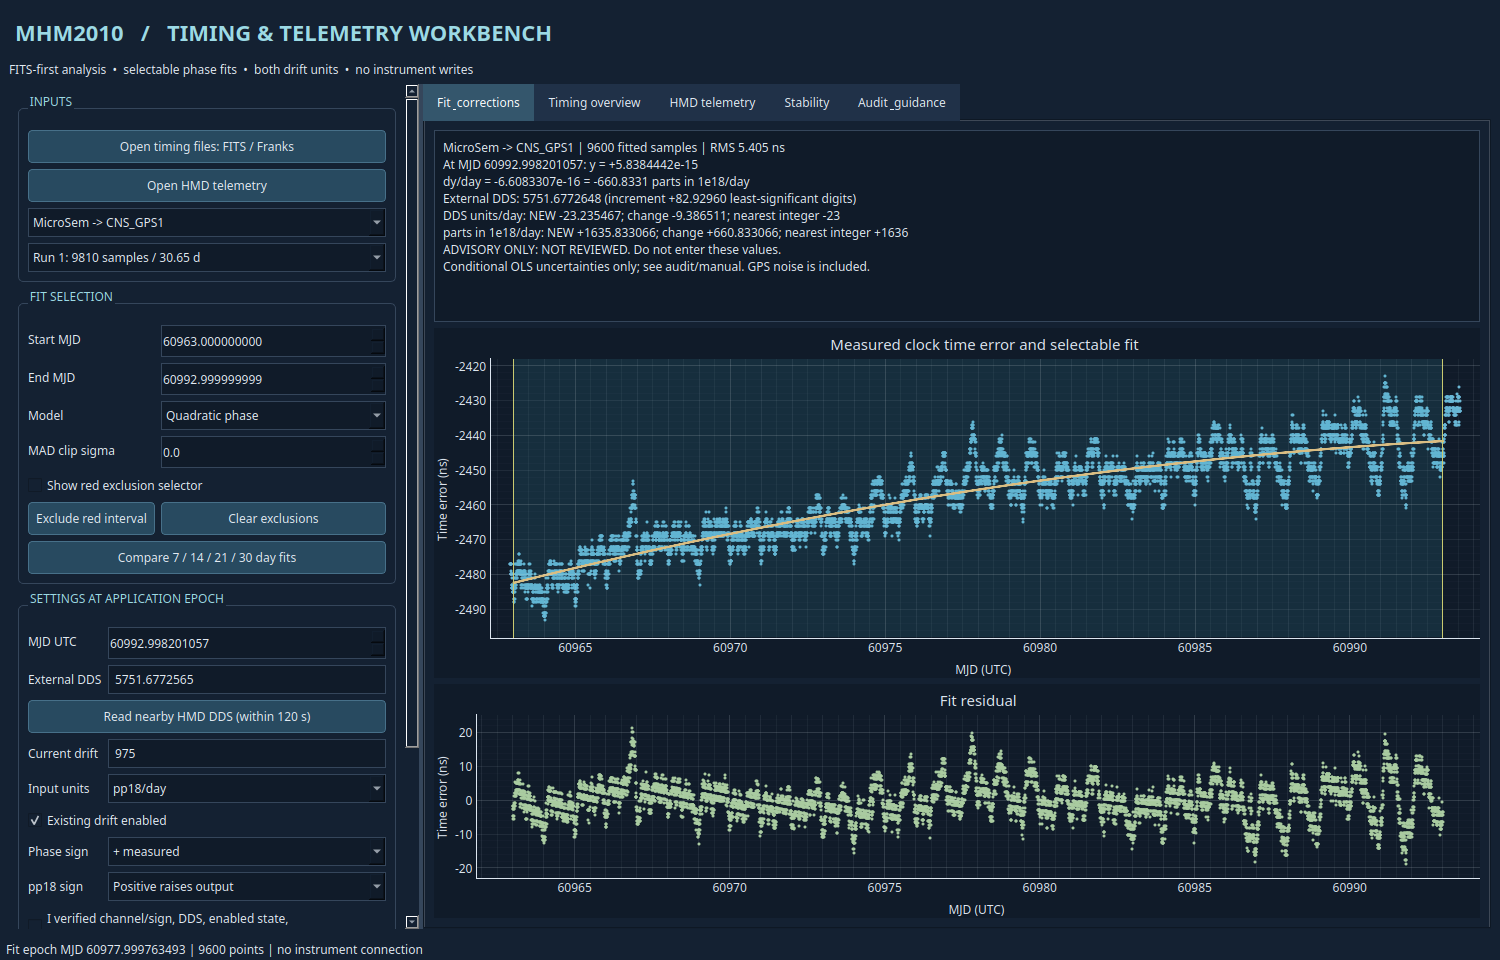
\includegraphics[width=\linewidth]{../validation/gui_fit.png}
\end{cfigure}
\textbf{Fit and corrections tab.} The blue region selects the fitting interval.
The phase and residual plots share their horizontal view. Numeric MJD limits
provide precise selection without requiring a mouse.

The red region is an independent exclusion selector. Add its interval to the
exclusion list or clear the list. Excluded observations remain in the input
and export, with an explicit used-in-fit mask. Optional iterative MAD residual
clipping is disabled by default. It can reject outliers, but it changes noise
statistics and must not conceal physical events.

A linear phase model estimates frequency only; the drift field is not
estimated and should not be changed on that basis. A quadratic phase model
estimates frequency and frequency drift. Internal scaling improves numerical
conditioning without changing the physical units of the returned coefficients.

The 7/14/21/30/90-day comparison button reports trailing-window fits in the audit
tab. These are unclipped quadratic diagnostic fits, with actual span and
sample count shown. They are not confidence intervals.

\begin{ctable}{GUI tabs of release 0.3.0, in order\label{tab:tabs}}
\begin{tabular}{@{}P{.3\linewidth}P{.65\linewidth}@{}}
\toprule
Tab & Content\\
\midrule
Fit and corrections & fit interval, exclusions, model, Results box with the suggested changes\\
1 PPS reference plots & the operator's two figures (deltas with statistics; data and fit over residuals)\\
Timing overview & every channel (hourly medians for FITS)\\
HMD telemetry & MHM2010 housekeeping columns and DDS events\\
T4 telemetry / T4 monitoring files & T4 MONIT and the T4's own logs\\
Stability & base OADEV, MDEV, OHDEV and TDEV (uniform record; section ``\nameref{sec:stability}'')\\
Eval: gap-aware stability & 0.3.0, section ``\nameref{sec:gapstab}''\\
Eval: steering removal & 0.3.0, section ``\nameref{sec:steering}''\\
Eval: Kalman estimate & 0.3.0, section ``\nameref{sec:kalman}''\\
Eval: three-cornered hat & 0.3.0, section ``\nameref{sec:tch}''\\
Audit \& guidance & audit trail, window comparison, export log\\
\bottomrule
\end{tabular}
\end{ctable}

\subsection{State and stale-result handling}
Changing the fit interval/model invalidates old stability results. In 0.3.0 the
evaluation results are invalidated too, by any change of the channel, fit, interval,
application epoch or phase sign; an export recalculates every ticked evaluation from the
current fit. Changing the channel clears the fit, candidate, suggestion and stability result
(the 0.2.4 stale-fit traceback is fixed). Settings can be saved without source-directory
paths, then restored after selecting the original files; they include the Veusz page choices
and the evaluation options. Restoring settings clears operator acknowledgments. Export
creates a new folder; it never silently replaces an earlier result directory.

\warning{The plots are interactive analysis of selected files, not streaming
acquisition. Large file reads run outside the GUI thread; fitting, overview
construction, evaluation and export may briefly occupy the GUI thread for very large
datasets. There is no serial or network maser interface in this release.}

\subsection{Time display: MJD or ISO 8601 calendar time}\label{sec:timedisplay}
Choose \textbf{View $\rightarrow$ Time display (axes, dates, ranges)}:
\begin{ctable}{Time display choices\label{tab:timedisplay}}
\begin{tabular}{@{}lll@{}}
\toprule
Menu entry & Example & Shortcut\\
\midrule
MJD (UTC) & \texttt{61349.86612} & Ctrl+Shift+M\\
Calendar date-time, local (ISO 8601) & \texttt{2026-11-05T15:47:13-05:00} & Ctrl+Shift+L\\
Calendar date-time, UTC (ISO 8601) & \texttt{2026-11-05T20:47:13+00:00} & Ctrl+Shift+U\\
\bottomrule
\end{tabular}
\end{ctable}
\begin{cfigure}{View menu: Time display (axes, dates, ranges).\label{fig:timemenu}}

\includegraphics[width=.75\linewidth]{../validation/gui_view_time_display_menu.png}
\end{cfigure}

The choice applies at once to: the fit, residual, HMD, overview, reference-figure, T4 telemetry,
T4 monitoring-file and evaluation time axes; the Start, End and application-epoch fields (they show
and accept the chosen form); the run list; the result text and status bar (calendar times keep the
MJD in brackets for the audit trail); and audit messages. It is remembered in
\texttt{workbench\_view.ini} beside the program and saved with the analysis settings. The data, fits
and exported numbers are always MJD (UTC); only the display changes. The \texttt{.vszh5} always
contains every time page against both MJD and local ISO time.

\textbf{Typing a time.} In calendar modes a field accepts \texttt{2026-11-05T15:47:13-05:00}, the one-digit
offset \texttt{-5:00}, \texttt{Z}, a date alone, a time without offset (read as local in local mode, UTC in
UTC mode) or a plain MJD. Up/down steps one hour (one day in MJD mode). The batch script's
\texttt{--start}/\texttt{--end} accept the same forms (no offset = UTC).

\textbf{Conversion and ticks.} The display converts as follows.
\begin{vartable}{tab:var-C}{Variables of the time-display conversion (C1)}
MJD & Modified Julian Date of the sample, UTC & day\\
\(t^{\mathrm{Unix}}\) & seconds since 1970-01-01T00:00:00 UTC (POSIX, no leap seconds) & s\\
\(t^{\mathrm{local}}\) & local wall-clock seconds on the same scale & s\\
\(o(t)\) & UTC offset of the processing computer at instant \(t\), daylight saving included & s\\
40587 & MJD of 1970-01-01 & day\\
\end{vartable}
\begin{equation}
t^{\mathrm{Unix}}=(\mathrm{MJD}-40587)\times86400\ \mathrm{s},\qquad
t^{\mathrm{local}}=t^{\mathrm{Unix}}+o(t^{\mathrm{Unix}}), \tag{C1}\label{eq:C1}
\end{equation}
so a July time at Green Bank shows \texttt{-04:00} and a November time \texttt{-05:00}. Ticks
fall on round calendar times (pyqtgraph's date logic, daylight-saving aware) and are labelled with
the full ISO time on two lines (date, then \texttt{Thh:mm:ss$\pm$hh:mm}); ticks closer than one label
width are dropped so labels never overlap. The axis title gives the offsets in the range, e.g.\
``Local date-time, ISO 8601 (UTC$-$05:00 then $-$04:00)''. ``Julian'' in common speech often means
this calendar view; strictly, MJD is the Julian-day count (JD$-$2\,400\,000.5) and the calendar
dates are Gregorian.

\begin{cfigure}{Local ISO 8601 display, last 90 days of the 2026 Franks MSM-GPS channel (Light theme).\label{fig:local90}}
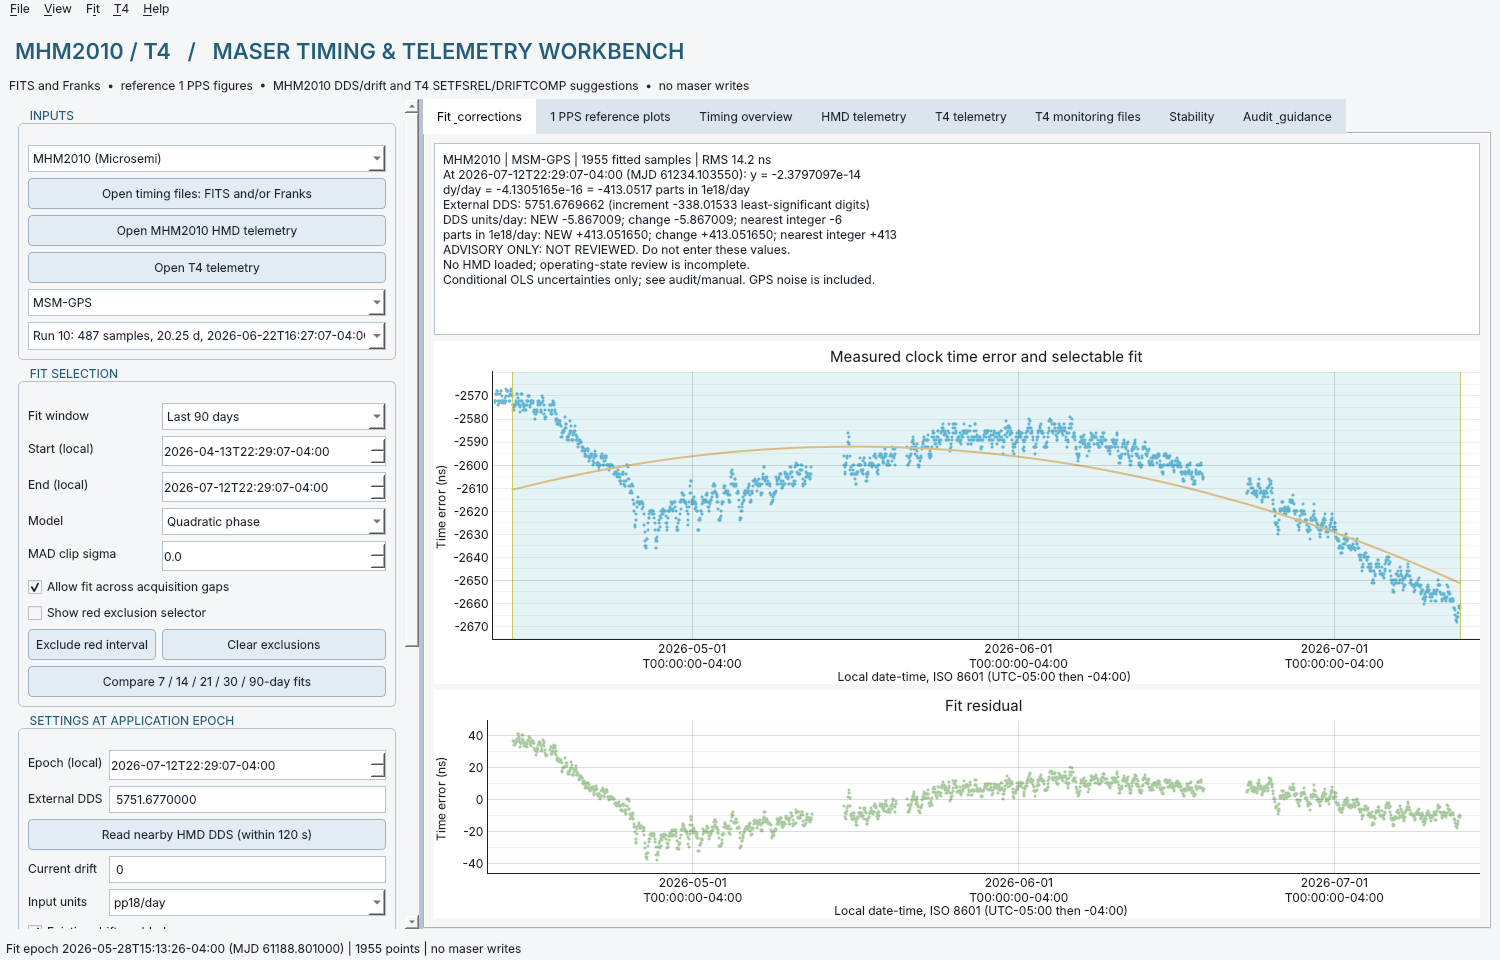
\includegraphics[width=.95\linewidth]{../validation/gui_time_display_local_90d_light.png}
\end{cfigure}

\subsection{Fit windows: last 7 to 90 days}
FIT SELECTION $\rightarrow$ \textbf{Fit window} (or the \textbf{Fit} menu) sets the blue interval to the
last 7, 14, 30 or 90 days ending at the last sample, or to all data, and moves the application epoch to
the last sample. A preset is enabled only when the loaded channel spans it (its tooltip gives the span
otherwise). If the window contains acquisition gaps, ``Allow fit across acquisition gaps'' is switched
on and logged; check the plot for phase steps. Dragging the blue interval returns to ``Custom''.
\textbf{Compare 7/14/21/30/90-day fits} (or Fit $\rightarrow$ Compare window lengths) fits each trailing
window ending at the selected end, skipping windows longer than the data; results go to the audit tab.
In batch, \texttt{--last-days 30} or \texttt{90} does the same and stops if the data are shorter.

On the 2026 Franks MSM-GPS data (193 days), the 90-day quadratic window ending 2026-07-13 02:29 UTC
gives $y=-2.38\times10^{-14}$ and drift $-413$ parts in $10^{18}$/day with 14.2~ns RMS; the 30-day
window gives $y=-3.71\times10^{-14}$, $-686$ parts in $10^{18}$/day and 3.6~ns RMS. The difference is
the window sensitivity this comparison exists to expose; the 90-day window spans gaps and a visible
phase excursion in April.
\clearpage
\section{Reference 1 PPS figures}\label{sec:reference}
The operator's two figures (the deltas with their statistics; the data and fit over the residuals)
are drawn in the GUI tab ``1 PPS reference plots'' and are the first pages of every
\texttt{analysis.vszh5}. They keep the operator's notation, so the symbols below are local to this
section (Appendix B lists them under ``Reference figures'').

\subsection{Definitions}
For the samples of a figure, the horizontal coordinate is days since the first sample shown and the
vertical coordinate is the 1 PPS time difference. The deltas figure uses every sample of the selected
interval; the fit figure uses the samples actually fitted (operator exclusions removed, drawn hollow and
grey).
\begin{vartable}{tab:var-R}{Variables of the reference 1 PPS figures (R1--R5)}
\(N_s\) & number of samples in the figure & 1\\
\(\mathrm{MJD}_i\), \(\mathrm{MJD}_0\) & time of sample \(i\); first sample shown & day\\
\(x_i\) & \(\mathrm{MJD}_i-\mathrm{MJD}_0\), horizontal coordinate & day\\
\(u_i\) & 1 PPS time difference of sample \(i\) (the figure's ``y'') & ns\\
\(\bar u\), std & mean and population standard deviation of \(u_i\) & ns\\
\(\bar x\) & mean of \(x_i\) & day\\
\(S_{xx}\), \(S_{xy}\) & \(\sum(x_i-\bar x)^2\); \(\sum(x_i-\bar x)(u_i-\bar u)\) & day\(^2\); ns\,day\\
\(a_1\), \(a_0\) & slope and intercept of the least-squares line \(u=a_1x+a_0\) (printed ``\(y=a_1x+a_0\)'') & ns/day; ns\\
\(r_i\) & residual \(u_i-a_1x_i-a_0\) & ns\\
\(\sigma^2\) & variance of independent residuals (model) & ns\(^2\)\\
\(s\) & residual standard deviation estimate, \(s^2=\sum r_i^2/(N_s-2)\) & ns\\
\(s(a_1)\), \(s(a_0)\) & standard errors of \(a_1\) and \(a_0\) & ns/day; ns\\
\(y_L\) & fractional frequency of the straight line (the figure's ``rate'') & 1\\
\(\epsilon\) & phase sign, \(\pm1\) (\(\epsilon u\) = maser minus reference) & 1\\
\(N\) & MHM2010 DDS setting (external synthesizer number) & DDS units\\
\(a\), \(q\) & \(2\times10^{-7}\) (DDS coefficient); \(10^{-7}\) (one count) & 1; DDS units\\
\(\Delta n\) & synthesizer adjustment of the figure & counts\\
\end{vartable}
The boxes report the mean and the population standard deviation (as \texttt{numpy.std}):
\begin{equation}
\bar u=\frac1{N_s}\sum_i u_i,\qquad
\mathrm{std}=\sqrt{\frac1{N_s}\sum_i (u_i-\bar u)^2}. \tag{R1}\label{eq:R1}
\end{equation}

\subsection{Straight-line fit and its standard errors}
The symbols are defined in Table~\ref{tab:var-R}. The least-squares line \(u=a_1x+a_0\) minimizes \(\sum r_i^2\). Setting
$\partial/\partial a_0=\partial/\partial a_1=0$ gives the normal equations, whose solution is
\begin{equation}
a_1=\frac{S_{xy}}{S_{xx}},\qquad a_0=\bar u-a_1\bar x . \tag{R2}\label{eq:R2}
\end{equation}
For independent residuals of variance $\sigma^2$, $\operatorname{Var}(a_1)=\sigma^2/S_{xx}$;
because $\operatorname{Cov}(\bar u,a_1)=0$,
$\operatorname{Var}(a_0)=\operatorname{Var}(\bar u)+\bar x^2\operatorname{Var}(a_1)
=\sigma^2\left(\frac1{N_s}+\frac{\bar x^2}{S_{xx}}\right)$. With $s^2$ in place of $\sigma^2$:
\begin{equation}
s(a_1)=\frac{s}{\sqrt{S_{xx}}},\qquad s(a_0)=s\sqrt{\frac1{N_s}+\frac{\bar x^2}{S_{xx}}},\qquad
y_L=\frac{a_1\,[\mathrm{ns/day}]\times10^{-9}}{86400\ \mathrm{s}} . \tag{R3}\label{eq:R3}
\end{equation}
These are conditional IID errors; colored noise and GPS systematics are not included \nist.
Check against the operator's figure: $N_s=741$, $s=3.49$~ns over 31 days gives
$S_{xx}\approx741\times31^2/12$, $s(a_1)\approx0.014$~ns/day and $s(a_0)\approx0.257$~ns, as printed.
The gap-aware stability and the Kalman estimate of 0.3.0 show how much larger the uncertainty is
when the identified noise is not white (section ``\nameref{sec:evalresults}'').

\subsection{Synthesizer adjustment line}
The symbols are defined in Table~\ref{tab:var-R}.
\textbf{MHM2010.} Appendix A gives the fractional change per DDS unit,
$\partial y/\partial N=-a/(284.08+aN)$ \manual. One count is $q=10^{-7}$ DDS units, so cancelling
$y=\epsilon y_L$ requires
\begin{equation}
\Delta n=\frac{-\epsilon y_L}{-aq/(284.08+aN)}
=\frac{\epsilon y_L\,(284.08+aN)}{2\times10^{-14}} . \tag{R4}\label{eq:R4}
\end{equation}
For $y_L=-3.15\times10^{-14}$ this is $-447$ counts, the value in the operator's figure; the
full DDS calculation of Appendix A agrees to $10^{-9}$ relative (test suite).

\textbf{T4.} The line shows the SETFSREL entry and the synthesizer change of section
``\nameref{sec:setfsrel}'' for the same straight-line rate.

\warning{The figure's adjustment uses the straight-line mean rate over the plotted span, as
the operator's figures do. The settings panel evaluates the selected model (linear or
quadratic) at the application epoch. With a quadratic fit the two can differ; enter only
the reviewed settings-panel values.}

\begin{cfigure}{GUI tab ``1 PPS reference plots'' (Light theme) on the operator's Franks files, June--July 2026, MSM-GPS.\label{fig:reference}}
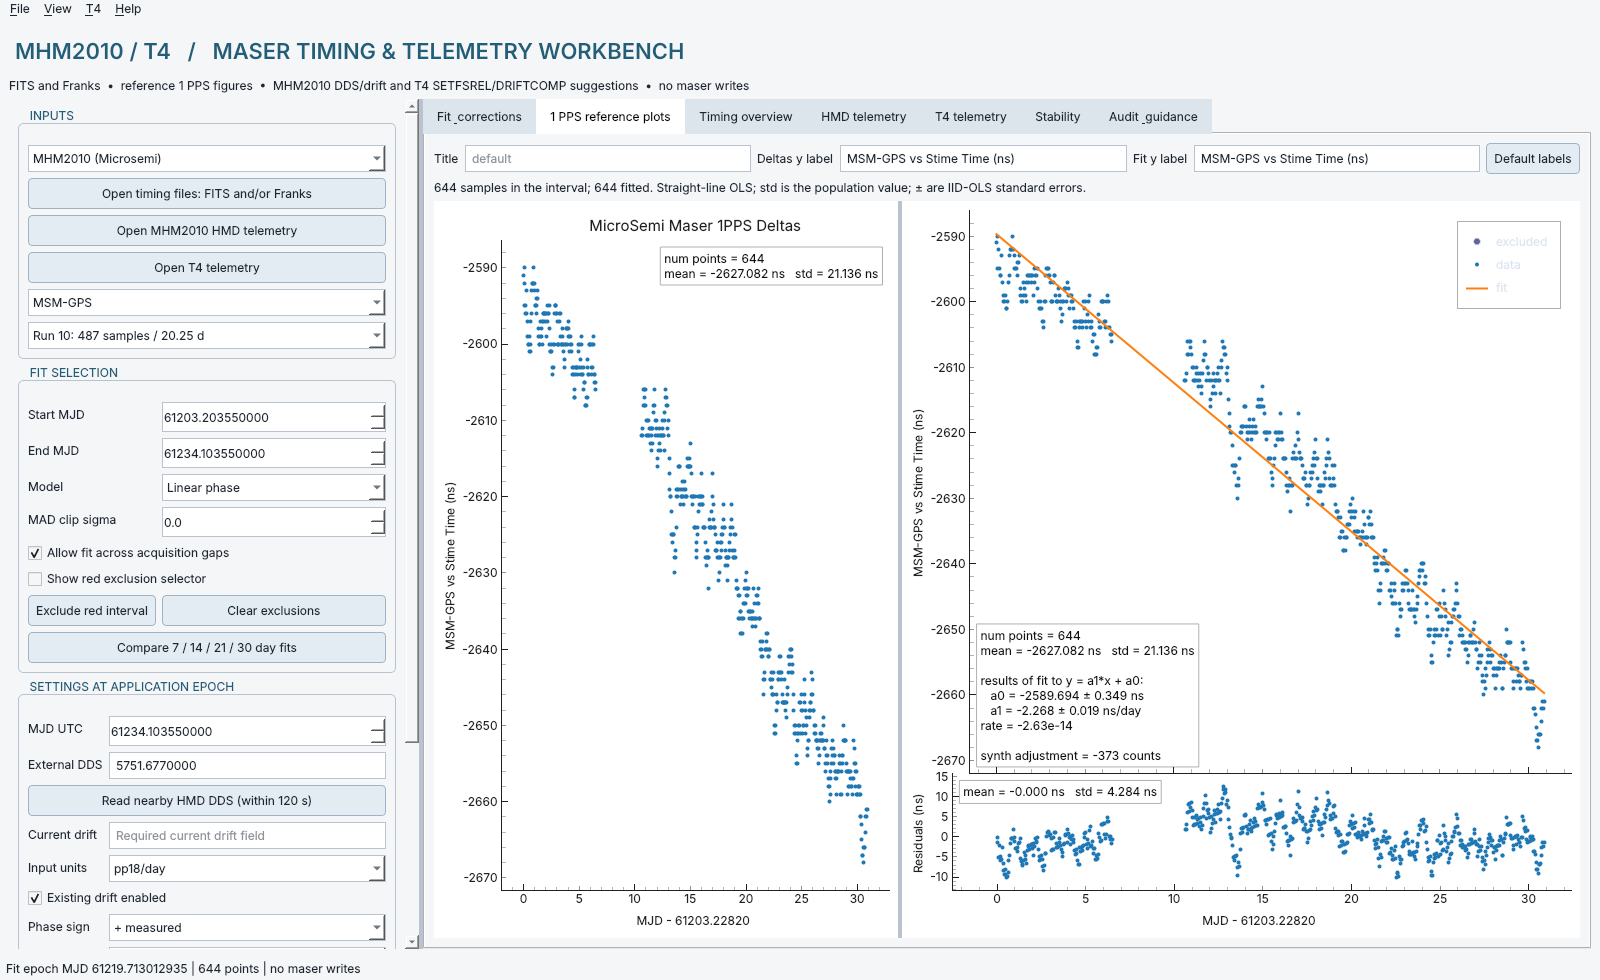
\includegraphics[width=\linewidth]{../validation/gui_reference_light.png}
\end{cfigure}
\clearpage

\section{Correction interpretation and manual review}
\subsection{One epoch, two absolute settings}
The phase fit is centered on an internal reference epoch. Frequency error is
evaluated at the separate intended application epoch. The old DDS must be the
setting at that application epoch, not the setting at the start of the data
or at the centered fit epoch.

The new external DDS is an \textbf{absolute setting}, not a number to add
again. Its displayed increment is also reported in least-significant DDS
digits. The new drift is the existing enabled drift plus a residual correction,
with the sign and units handled explicitly. An existing disabled drift
contributes zero regardless of a stale numeric value in its field.

The pp18/day input field and DDS-units/day input field are alternative
representations of the same ramp. The program reports both new values and
both increments. Do not apply both increments sequentially.

\subsection{Sign and precision}
For the adopted timing definition, measured arrival(B) minus arrival(A)
equals clock(A) minus clock(B). A direct MicroSem-to-GPS pair therefore uses
the positive sign; a reverse pair uses the negative sign. This channel
interpretation must be checked against the installed measurement wiring and
logging convention.

Positive physical DDS units/day means the DDS number increases with time,
which lowers output frequency \manual. The installed pp18 sign is separately
selectable: positive raises output frequency, or positive raises DDS. The
default is an explicit assumption, not a claim that Rev. J documents that sign.

The external DDS is rounded to seven decimal places. Both drift values are
also shown without integer rounding and with nearest-integer alternatives.
The integer alternatives are illustrative: verify what entry precision the
installed masermon accepts. pp18 integer increments and DDS integer increments
do not have the same effective frequency-drift resolution.

\subsection{Before entering any candidate}
\begin{itemize}
\item \textbf{Reference}: confirm the GPS channel is healthy, not stepped or being steered unexpectedly.
\item \textbf{Instrument}: confirm external synthesizer selection, current DDS, drift enable state and units.
\item \textbf{Sign}: verify the instrument's installed pp18 convention; do not test it by an uncontrolled adjustment.
\item \textbf{Time}: use a current, defensible application epoch and known setting at that epoch.
\item \textbf{Fit}: inspect residuals, HMD changes, outages and window sensitivity.
\item \textbf{Evaluation (0.3.0)}: compare the base drift with the steering-removed drift and the Kalman
uncertainty; a drift change smaller than its Kalman \(1\sigma\) is not supported by the data.
\item \textbf{Record}: preserve old settings, intended values, operator review and subsequent comparison data.
\end{itemize}

No checkbox turns this software into a certified controller. Values remain
advisory even after the operator review fields are acknowledged.
\clearpage

\section{Suggested settings: frequency and drift}\label{sec:suggested}
\subsection{Equations}
The suggestion is made from the selected phase model and the channel sign at the application
epoch, with the DDS relations of Appendix A, equations (A13)--(A19). The symbols are those of
Appendix A.
\begin{vartable}{tab:var-S}{Variables of the suggested settings (S1--S4)}
\(c_0,c_1,c_2\) & phase-model coefficients, \(x=c_0+c_1d+c_2d^2\) & ns; ns/day; ns/day\(^2\)\\
\(d\), \(d_a\) & elapsed days (SI) from the fit epoch; at the application epoch & day\\
\(\epsilon\) & phase sign, \(\pm1\) (\(\epsilon x\) = maser minus reference) & 1\\
\(y\) & residual fractional frequency of the maser at the application epoch & 1\\
\(r\) & residual fractional-frequency drift & day\(^{-1}\)\\
\(N\), \(N_{\mathrm{new}}\) & current and new DDS setting & DDS units\\
\(a\) & DDS coefficient \(2\times10^{-7}\) \manual & 1\\
\(D\) & synthesizer denominator \(284.08+aN\) (nominal 284.08 when \(N\) is not entered) & 1\\
\(k_N\) & \(a/D\), fractional output change per DDS unit (magnitude) & DDS units\(^{-1}\)\\
\(q\) & one DDS count, \(10^{-7}\) & DDS units\\
\(\eta\) & pp18 sign convention: \(+1\) positive raises output, \(-1\) positive raises DDS & 1\\
\(\Delta n\) & DDS change & counts\\
\(\Delta P\) & drift-field change in pp18/day & \(10^{-18}\)/day\\
\(\Delta v\) & drift-field change in DDS counts/day & counts/day\\
\(v_{\mathrm{old}}\) & current drift field in DDS counts/day & counts/day\\
\(\mathrm{round}_q\) & rounding to a multiple of \(q\) & --\\
\end{vartable}
\begin{align}
y&=\epsilon\,\frac{(c_1+2c_2d_a)\,10^{-9}}{86400},\qquad
r=\epsilon\,\frac{2c_2\,10^{-9}}{86400}\ \text{per day}, \tag{S1}\label{eq:S1}\\
\Delta n&=\frac{D}{a}\,\frac{y}{q}\quad\text{(DDS change, counts)},\tag{S2}\label{eq:S2}\\
\Delta P&=-\eta\,\frac{r}{1+y}\,10^{18}\quad\text{(drift change, pp18/day)},\tag{S3}\label{eq:S3}\\
\Delta v&=\frac{r}{k_N q}\ \bigl(+\,v_{\mathrm{old}}\,y\ \text{when the current field is in DDS counts/day}\bigr)
\quad\text{(drift change, DDS counts/day)}.\tag{S4}\label{eq:S4}
\end{align}
Without a DDS setting the nominal \(D=284.08\) is used (a relative change of \(4\times10^{-6}\) at
\(N=5752\)). With the current values: \(N_{\mathrm{new}}=\operatorname{round}_q(N+q\Delta n)\) and
drift field \(=\) current \(+\) change. T4: \texttt{SETFSREL} from Eq.~12 of \tfourman\ (39-bit step,
equation (F4)) and \(\mathtt{DRIFTCOMP}_{\mathrm{new}}=\mathtt{DRIFTCOMP}_{\mathrm{now}}-r\)
\tfournet\ (equation (D3), with \(r\) already carrying \(\epsilon\)). A linear model estimates no drift;
the box then says so. The arithmetic is the same as \texttt{correction()} and \texttt{t4\_settings()}
(tested to \(10^{-13}\) or identical). In 0.2.4 the same equations were written with \(a_0,a_1,a_2\),
\(\tau\) and \(D\) for the coefficients, the days and the drift; the symbols are now those of
Appendix A, and the arithmetic is unchanged.

\subsection{Where the two changes are stated}
\begin{ctable}{Where the suggested frequency and drift changes appear\label{tab:suggestwhere}}
\begin{tabular}{@{}P{.3\linewidth}P{.62\linewidth}@{}}
\toprule
Place & Content\\
\midrule
Fit \& corrections, Results & ``SUGGESTED CHANGES'': the box text plus the exact values and notes;
below, the new absolute settings when the current DDS and drift are entered\\
1 PPS reference plots, fit figure & box ``suggested \ldots\ changes'' at the upper left; the y axis
leaves room above the data so the box never covers points\\
\texttt{analysis.vszh5} & the same box on \texttt{Ref1PPS\_<channel>\_fit\_MJD} and \texttt{\_fit\_local};
datasets \texttt{Suggested\_<maser>\_*} (one value each, exact), \texttt{\_full\_precision\_text},
\texttt{\_box\_text}\\
\texttt{analysis.json}, \texttt{review.md} & \texttt{suggested\_settings}; exact-value table\\
\texttt{analyze\_maser.py} & printed \texttt{suggested\_settings}\\
Eval: Kalman estimate (0.3.0) & settings from the Kalman estimate, marked EVALUATION ONLY; never in the
box, the Results or \texttt{suggested\_settings}\\
\bottomrule
\end{tabular}
\end{ctable}

\subsection{Example: last 30 days of the 2026 Franks MSM-GPS data}
\begin{itemize}
\item Quadratic phase, 622 points; epoch \texttt{2026-07-12T22:29:06.72-04:00} (MJD 61234.10355).
\item \(y=-3.708732994065008\times10^{-14}\); \(r=-6.864816602325095\times10^{-16}\)/day.
\item \textbf{DDS change \(-526.79\pm10.49\) counts; drift change \(+686.48\pm47.16\) pp18/day
\(=-9.7508\) DDS counts/day} (positive pp18 raises the output).
\item With DDS 5751.6770000 and drift \(-120\) pp18/day: new DDS 5751.6769473 and new drift field
\(+566.48\) pp18/day.
\end{itemize}
The straight-line
``synth adjustment'' of the same figure is \(-379.26\) counts (interval-mean rate); the quadratic
gives \(-392.00\) counts at the mean sample time (MJD 61220.28; uneven sampling around the 5-day gap)
and \(-526.79\) at the end, \(13.82\,\mathrm{d}\times9.75\) counts/day later. The \(\pm\) values are
conditional OLS uncertainties; GPS and colored noise are not included.
\begin{cfigure}{Veusz 3.6.2 render of \texttt{Ref1PPS\_MSM\_GPS\_fit\_MJD}: the figure's results box (lower left) and the suggested-changes box (upper left).\label{fig:refbox}}
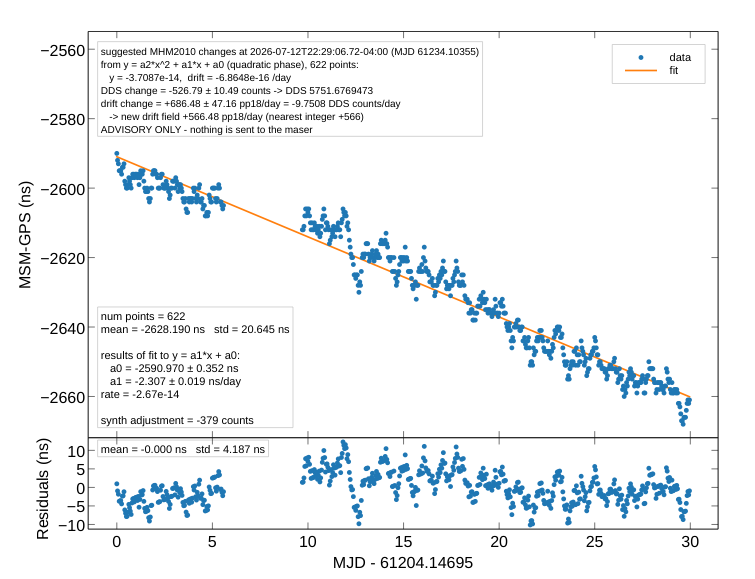
\includegraphics[width=.86\linewidth]{../validation/veusz_render_v0.2.4/analysis_p01_Ref1PPS_MSM_GPS_fit_MJD.png}
\end{cfigure}
\begin{cfigure}{The GUI with empty DDS and drift fields: both changes are stated.\label{fig:refsuggest}}
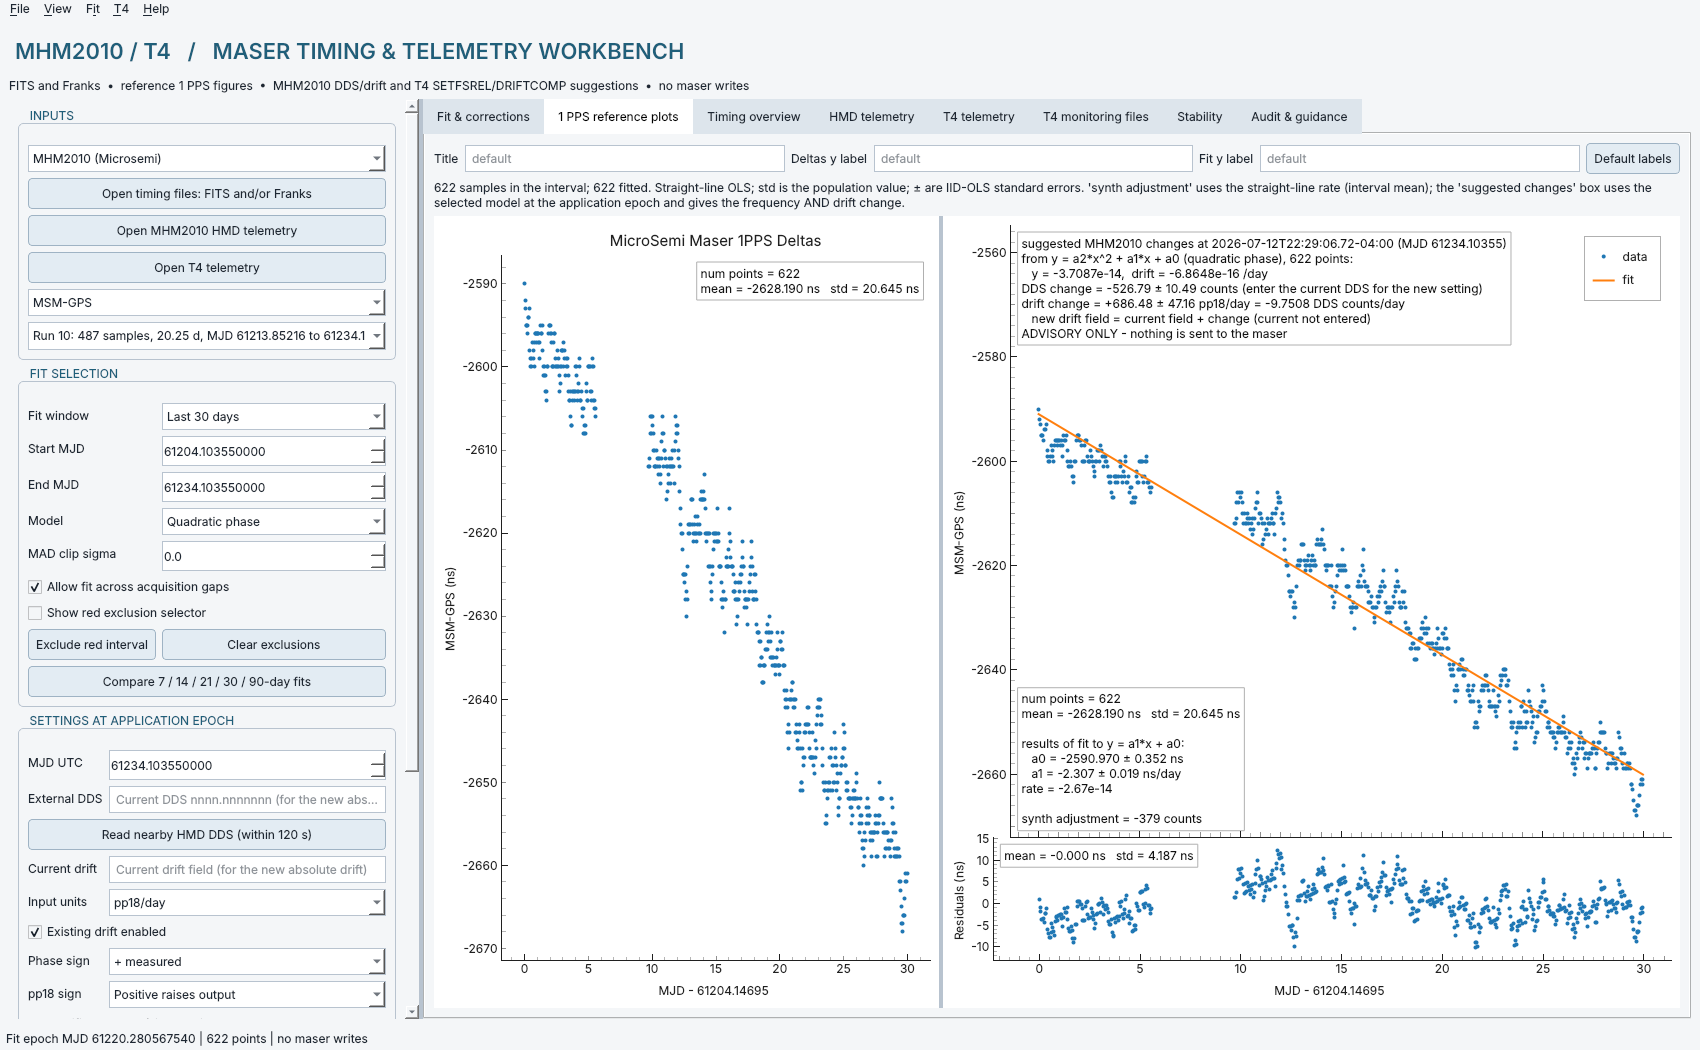
\includegraphics[width=.95\linewidth]{../validation/gui_reference_suggestions_light.png}
\end{cfigure}
\warning{Enter only reviewed values. Confirm the pp18 sign convention of the installed masermon,
the channel sign, the epoch and the maser state; the HMD shows whether a drift is already acting on
the DDS.}
\clearpage

\section{T4 iMaser 3000}
\subsection{MONIT telemetry}
The reply to \texttt{MONIT;} is \texttt{\$} + 113 hexadecimal characters + CR LF (Type 1, Card
FPGA T4S-724) or CR (Type 2, IO card LAN T4S-711) \tfourman. The channels are 32 of 12 bits,
8 of 8 bits and the main-PLL lock bit.
\begin{vartable}{tab:var-M}{Variables of the MONIT decoding (M1)}
\(L_{\mathrm{hex}}\) & number of hexadecimal characters after \texttt{\$} & characters\\
\(i\) & channel number, 1 to 41 & 1\\
\(\text{field}_i\) & hexadecimal field of channel \(i\) (3 or 2 characters, or the lock bit) & --\\
\(c_i\) & unsigned integer code of channel \(i\) & code\\
\(g_i\) & gain of channel \(i\), Table 6 of \tfourman\ (negative for the \(-15\)~V rail) & V/code (or unit/code)\\
\(v_i\) & decoded value of channel \(i\) & V (or channel unit)\\
\end{vartable}
\begin{equation}
L_{\mathrm{hex}}=32\cdot3+8\cdot2+1=113,\qquad v_i=g_i\,c_i,\quad c_i=\texttt{int}(\text{field}_i,16). \tag{M1}\label{eq:M1}
\end{equation}
Gains $g_i$ are Table 6 of \tfourman, identical to the operator's repository table \tfoursrc;
the $-15$~V rail has a negative gain. Channels 21, 37 and 39 are ``Not used''. Channel 40
(LOCK 100~MHz) is an 8-bit analog voltage; channel 41 is the lock bit (1 locked, 0 unlocked;
any other code is flagged). Decoding the manual's example reply gives 4.765~V for channel 40;
the operator's web-page screenshot shows 4.764~V.

\textbf{Inputs.} The recorder's \texttt{t4\_raw\_frames.csv} (re-decoded from the raw replies),
its \texttt{t4\_telemetry.csv} (raw codes re-scaled), or text logs with one
\texttt{<time> \$<frame>} per line. Times must be MJD or ISO~8601 with an offset.

\textbf{Live polling} (T4 tab) sends only \texttt{MONIT;}, \texttt{RDFS;}, \texttt{GETID;} and
\texttt{RDREG=\dots;} over UDP port 14000 \tfournet. Each attempt uses a fresh socket with bounded
retries; datagrams from other peers are ignored. Since 0.2.1 the local UDP port defaults to
14000 for a real T4: the vendor example and \texttt{T4\_Maser\_Comms.py} bind it (``seems one
must bind the port to local port as well'' \tfoursrc), so the T4 probably answers to port 14000
rather than to the sender's port; the manual does not say. The emulator uses an ephemeral port.
Raw replies are written before decoding, into a folder stamped once at creation
(\texttt{T4\_telemetry\_YYYYMMDDTHHMMSS±hhmm}). The preview buffer is bounded and can be flushed or
offloaded to a pickle. A non-loopback address requires the approval box. ``Use loopback emulator''
serves the manual's example reply. Since 0.2.4 the recorder CSVs write MJD, round-trip time and
channel values with every digit, and the UTC text is exact.

\subsection{Frequency setting: SETFSREL}\label{sec:setfsrel}
The PLL forces the last IF to equal the synthesizer frequency and the output is the 5~MHz OCXO
(\tfourman, Eqs.~10--12, Sec.~9.4).
\begin{vartable}{tab:var-F}{Variables of the T4 frequency setting (F1--F5)}
\(F_{\mathrm{out}}\) & hydrogen-maser oscillation frequency in the T4 relations (fixed) & Hz\\
\(\nu_{\mathrm{ocxo}}\), \(\nu_0\) & OCXO frequency; output frequency (\(\nu_0=\nu_{\mathrm{ocxo}}\approx5\)~MHz) & Hz\\
\(\nu_{\mathrm{synth}}\) & synthesizer frequency (read with \texttt{RDFS}) & Hz\\
\(\Delta\nu_{\mathrm{synth}}\), \(\Delta\nu_0\) & change of synthesizer and of output frequency & Hz\\
\(y_0\) & fractional output change produced by \(\Delta\nu_{\mathrm{synth}}\) & 1\\
\(y\) & measured fractional frequency offset of the T4 (maser minus reference) & 1\\
\(\Delta y\) & output change required, \(-y\) & 1\\
\(q_T\) & synthesizer resolution \(5\ \mathrm{MHz}/2^{39}=9.0949\times10^{-6}\) & Hz\\
\(n_T\) & integer number of synthesizer steps & steps\\
\(\Delta y_{\mathrm{realized}}\) & output change after quantization & 1\\
\texttt{SETFSREL} & entered relative step, mandatory sign, range \(\pm29\times10^{-9}\) \tfournet & s/s\\
\(\mathrm{RDFS}_{\mathrm{pred}}\) & predicted \texttt{RDFS} after the entry & Hz\\
\end{vartable}
\begin{align}
\nu_{\mathrm{synth}}&=F_{\mathrm{out}}-284\,\nu_{\mathrm{ocxo}},\qquad
\nu_0=\nu_{\mathrm{ocxo}}=\frac{F_{\mathrm{out}}-\nu_{\mathrm{synth}}}{284}, \tag{F1}\label{eq:F1}\\
y_0&=\frac{\Delta\nu_0}{\nu_0}=\frac{-\Delta\nu_{\mathrm{synth}}}{284\times5\ \mathrm{MHz}}
=\frac{-\Delta\nu_{\mathrm{synth}}}{1.42\times10^{9}\ \mathrm{Hz}}\qquad(\text{Eq.~12 of \tfourman}), \tag{F2}\label{eq:F2}\\
\Delta y&=-y\ \Rightarrow\ \Delta\nu_{\mathrm{synth}}=y\times1.42\times10^{9}\ \mathrm{Hz},
\qquad q_T=\frac{5\ \mathrm{MHz}}{2^{39}}, \tag{F3}\label{eq:F3}\\
n_T&=\operatorname{round}\!\left(\frac{\Delta\nu_{\mathrm{synth}}}{q_T}\right),\qquad
\Delta y_{\mathrm{realized}}=-\frac{n_T\,q_T}{1.42\times10^{9}\ \mathrm{Hz}},\qquad
\texttt{SETFSREL}=\pm\Delta y_{\mathrm{realized}}, \tag{F4}\label{eq:F4}\\
\mathrm{RDFS}_{\mathrm{pred}}&=\nu_{\mathrm{synth}}+n_T\,q_T . \tag{F5}\label{eq:F5}
\end{align}
The resolution \(q_T\) is \(6.405\times10^{-15}\) relative.
\tfournet\ defines SETFSREL as a relative step in s/s with a mandatory sign, but not whether $+$
raises the output. The selector ``SETFSREL sign'' sets the convention, and the panel predicts the new
\texttt{RDFS} value (F5), which must lie within 405\,708--405\,795~Hz. \textbf{After entry, compare
RDFS with the prediction}; a move in the opposite direction means the convention is
reversed. RDFS values near 1.42~GHz (the web page's FREQ) are reduced by $1.42\times10^9$~Hz.

\subsection{Drift: DRIFTCOMP}
With linear drift the T4 manual models frequency and phase as below (\tfourman, Eqs.~22--23); the
quadratic phase fit of Appendix A gives the same quantities.
\begin{vartable}{tab:var-D}{Variables of the T4 drift setting (D1--D3)}
\(t\) & time since the start of the model & s\\
\(y(t)\), \(y_0\) & fractional frequency; its value at \(t=0\) & 1\\
\(\dot y\) & fractional-frequency drift & s\(^{-1}\)\\
\(x(t)\), \(x_0\) & phase (time error); its value at \(t=0\) & s\\
\(c_0,c_1,c_2\), \(d\) & phase-fit coefficients and elapsed days (Appendix A) & ns, ns/day, ns/day\(^2\); day\\
\(r\) & drift per day, \(r=\dot y\times86400\) s from the fit & day\(^{-1}\)\\
\(\epsilon\) & phase sign, \(\pm1\) & 1\\
\(\mathtt{DRIFTCOMP}_{\mathrm{now}}\), \(\mathtt{DRIFTCOMP}_{\mathrm{new}}\) & current (\texttt{RDREG=DRIFTCOMP;}) and new drift compensation & day\(^{-1}\)\\
\end{vartable}
\begin{align}
y(t)&=y_0+\dot y\,t,\qquad x(t)=x_0+y_0t+\tfrac12\dot y\,t^2, \tag{D1}\label{eq:D1}\\
y&=\frac{(c_1+2c_2d)\,10^{-9}}{86400},\qquad r=\frac{2c_2\,10^{-9}}{86400}, \tag{D2}\label{eq:D2}\\
\mathtt{DRIFTCOMP}_{\mathrm{new}}&=\mathtt{DRIFTCOMP}_{\mathrm{now}}-\epsilon\,r,
\qquad 10^{-17}<|\mathtt{DRIFTCOMP}|<8\times10^{-13}. \tag{D3}\label{eq:D3}
\end{align}
``A positive sign will generate a positive slope compensation'' \tfournet, hence the minus sign in
(D3). The entry is followed by REBOOT, which ``Reboot[s] the M\&C software'' (\tfournet, Table~1,
p.~8), and \texttt{RDREG=DRIFTCOMP;} to verify. Neither command removes the 1~PPS time offset
(ADJ1PPS/SYNCPPS).

\begin{ctable}{T4 demonstration with MSM-GPS as a stand-in (not T4 data)\label{tab:t4demo}}
\begin{tabular}{@{}lr@{}}
\toprule
Quantity & Value\\
\midrule
Fit: last 30.9 d of 2026 Franks MSM-GPS, quadratic, gap bridged & 644 samples\\
$y$ at MJD 61234.10355 & $-3.7365\times10^{-14}$\\
$\Delta\nu_{\mathrm{synth}}$, steps & $-54.570~\mu$Hz, $-6$\\
Suggested entry (``+ raises output'') & \texttt{SETFSREL=+3.843E-14;}\\
RDFS before $\rightarrow$ predicted after & 405750.927598720 $\rightarrow$ 405750.927544150 Hz\\
Drift entry (current 0) & \texttt{DRIFTCOMP=+7.11e-16;}\\
\bottomrule
\end{tabular}
\end{ctable}

\warning{No FITS pair or Franks column is identified as the T4 yet. Designate the channel
in the GUI (``Selected channel is the T4 comparison'') or with \texttt{--maser T4 --channel}.
T4 settings stay blocked until the channel is designated.}

\section{T4 monitoring files (FTP ./Monitoring)}
\subsection{What the manual says}
\texttt{RECMONIT=<s>;} records the monitoring ``in a file stored on the local SD memory card'';
the file ``can be accessed by FTP under the directory ./Monitoring''; at 2~MB it ``is copied
with a tag of the date and time, and the current file is reset'' (\tfournet, Sec.~1.1.3, p.~12;
Sec.~6.5, p.~22). RECMONIT appears only in Sec.~1.1.3, not in the Table~1 command list. The web
page shows only whether recording is ON or OFF (Sec.~1.1.3, p.~12; Sec.~4, p.~20). Each record
is tagged with the module's date and time, set by NTP or \texttt{SETDATE}/\texttt{SETTIME}; without
synchronisation at power-up the clock is not kept (pp.~12, 22). Option telemetry such as the HCB
is recorded in these files although \texttt{MONIT} does not return it (p.~14). The FTP login is in
Sec.~6.1 (p.~21). The manual does not document file names, columns or the record layout.

\subsection{Format, as found in the GBO file}
\begin{ctable}{Format of the GBO T4 monitoring file \texttt{MonitHCB.dat}\label{tab:monithcb}}
\begin{tabular}{@{}P{.25\linewidth}P{.69\linewidth}@{}}
\toprule
Property & \texttt{MonitHCB.dat}, GBO T4, received 2026-11-05\\
\midrule
Layout & Tab-separated; CR~LF; header \texttt{TIME} then \texttt{Label [unit]} per column\\
Encoding & UTF-8; the degree sign arrived as U+FFFD (bytes EF BF BD) and is repaired to \textdegree\\
Time & \texttt{DD/MM/YY HH:MM:SS}, UTC, 1~s resolution\\
Records & 84: 10 before the time-server sync (3 stamped 2006-01-16, 7 stamped 2007-06-06), then 74
from 17:13:09 to 18:25:39 UTC\\
Interval & median 60~s, mean 59.59~s, range 59--62~s\\
Columns & Set, Internal and External temperature [\textdegree C]; Alarm Status (text)\\
\bottomrule
\end{tabular}
\end{ctable}
\textbf{Date order.} \texttt{16/01/06} cannot be MM/DD (no month 16), and YY/MM/DD would date the
newest records to 2005. The last record, 05/11/26 18:25:39, was 1.5~min before the file reached
this computer (13:27 EST = 18:27 UTC), consistent with UTC as the operator stated. DMY is the
default; the reader warns when another order would read every line that the chosen order cannot
(a wrong order can still read most lines: \texttt{05/11/26} is a valid MM/DD/YY).

\subsection{Time base and clock-not-set rule}
The records carry the maser's own stamps (unlike MONIT rows, which carry this computer's receive
time) and may be compared with timing data directly.
\begin{vartable}{tab:var-L}{Variables of the monitoring-file time base and interval statistics (L1--L3)}
\(t\), \(t^{\mathrm{Unix}}\) & record time in seconds since 1970-01-01 UTC & s\\
MJD & Modified Julian Date of the record & day\\
\(t_{\mathrm{min}}\) & earliest valid time, ``Clock valid from'' (default 2020-01-01 UTC) & s\\
\(t_{\mathrm{now}}\) & time of reading & s\\
\(t_k\) & successive clock-valid record times & s\\
\(\Delta_k\) & interval between successive records & s\\
\end{vartable}
\begin{gather}
\mathrm{MJD}=\frac{t^{\mathrm{Unix}}}{86400\ \mathrm{s}}+40587, \tag{L1}\label{eq:L1}\\
\text{clock-valid:}\quad t_{\mathrm{min}}\le t\le t_{\mathrm{now}}+1\ \mathrm{d}, \tag{L2}\label{eq:L2}\\
\Delta_k=t_{k+1}-t_k,\qquad \text{gap if}\ \Delta_k>1.5\,\operatorname{median}(\Delta). \tag{L3}\label{eq:L3}
\end{gather}
So 2026-11-05 17:13:09 UTC is MJD $61349+\frac{62\,089}{86\,400}=61349.717465$. Records that are not
clock-valid (L2) are listed in the table and CSV (greyed, \texttt{clock\_valid}=0, with their file and
line) but never plotted or analysed (``Clock valid from'' in the tab, \texttt{--t4-earliest-valid} in
batch). Runs of such records are reported separately; a new run starts at a jump of more than 1~h or
backwards. Interval statistics use clock-valid records only: the median, mean, minimum and maximum of
\(\Delta_k\), the count of \(\Delta_k<0\), and the count of gaps (L3).

\subsection{HCB columns}
HCB is the Active Heater-Cooler-Box option (climatic chamber) [13]; the SMC unit sets the
temperature of the liquid circulating in its tubes (\texttt{SETTEMPHCB}). The HTML page shows ``the
setting of the temperature'', ``the internal temperature sensor used for regulation'', ``the
external temperature sensor if used'' and ``the operation status normal or Alarm (the error code
of the error will be displayed)'' (\tfournet, Sec.~1.1.3, p.~16). In the GBO file, set point and
internal temperature are 21.5~\textdegree C throughout the clock-valid span (22~\textdegree C in the
2006 pre-sync records), the external temperature is a constant 80~\textdegree C, and the status is
``No error''. A constant 80~\textdegree C suggests that no external sensor is connected; this is an
inference, not confirmed. Status text is kept as written and plotted as a flag: 0 for ``No error'',
1 otherwise.

\subsection{Reading several files}
Files with the same header (the live file and its rolled, date-tagged copies) are merged in order of
their latest record, so a pre-sync 2006 stamp cannot put the newest file first. Identical records
(same time and values) are kept once; records with the same time but different values are kept and
reported. Files with different headers stay separate logs. Files are read in parallel threads; at
most 2~MB each \tfournet, they need no special memory handling, and ``Clear from RAM'' releases them.

\subsection{Outputs and use}
\begin{itemize}
\item \textbf{GUI}: open with File $\rightarrow$ Open T4 telemetry or monitoring files (Ctrl+T), the
T4 menu, or drag and drop; files are routed by content (a tab-separated header starting with
\texttt{TIME}). The tab shows one x-linked plot per column against $\mathrm{MJD}-\mathrm{MJD}_0$,
UTC or local date-time, the summary and notes, and every record.
\item \textbf{Export}: \texttt{t4\_<layout>\_records.csv} (every record, clock flag, source line;
UTF-8 with BOM), \texttt{t4\_telemetry.json}, and \texttt{t4\_telemetry.vszh5} with one panel per
column (each with its own range, padded by 10\,\% or $\pm0.5$ when constant), a status page and a
notes page, each against $\mathrm{MJD}-\mathrm{MJD}_0$ and against local ISO time.
\item \textbf{Batch}: \texttt{analyze\_maser.py --t4-telemetry MonitHCB.dat \dots} adds the pages to
\texttt{analysis.vszh5} (leave them out with \texttt{--no-t4-monitoring-plots});
\texttt{python t4\_native.py MonitHCB.dat --output NEW\_DIR} exports only the monitoring files.
\end{itemize}
\begin{cfigure}{Tab ``T4 monitoring files'' (Light theme, local date-time axis) on the GBO \texttt{MonitHCB.dat}.\label{fig:t4mon}}
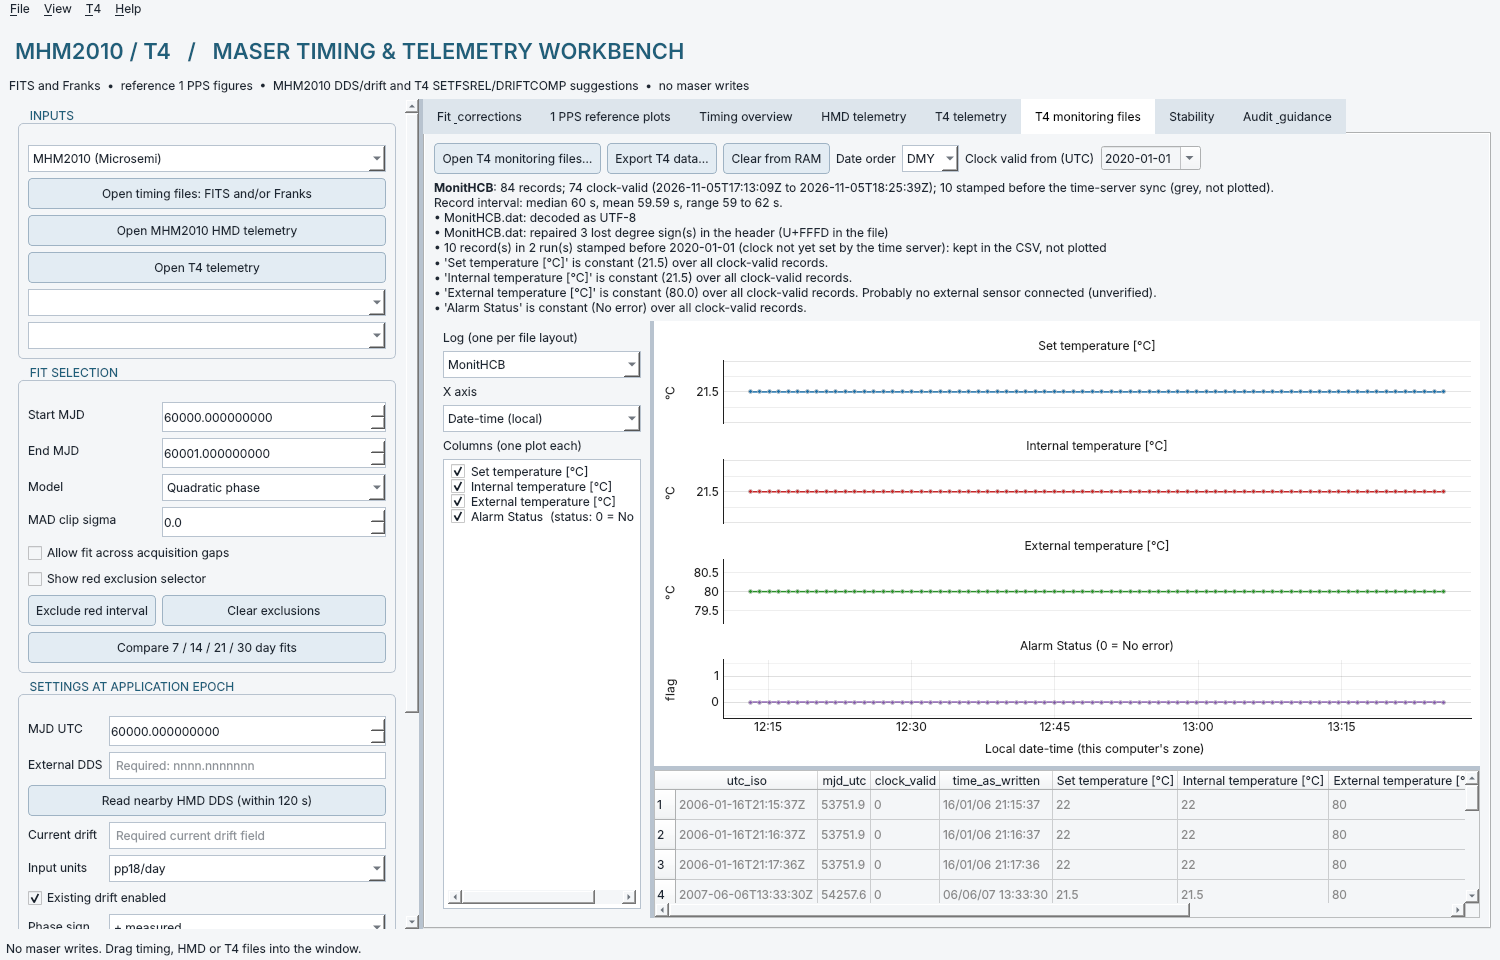
\includegraphics[width=.92\linewidth]{../validation/gui_t4_monitoring_light.png}
\end{cfigure}
\begin{cfigure}{Veusz 3.6.2 render of the exported monitoring page against local ISO time (EST).\label{fig:t4monveusz}}
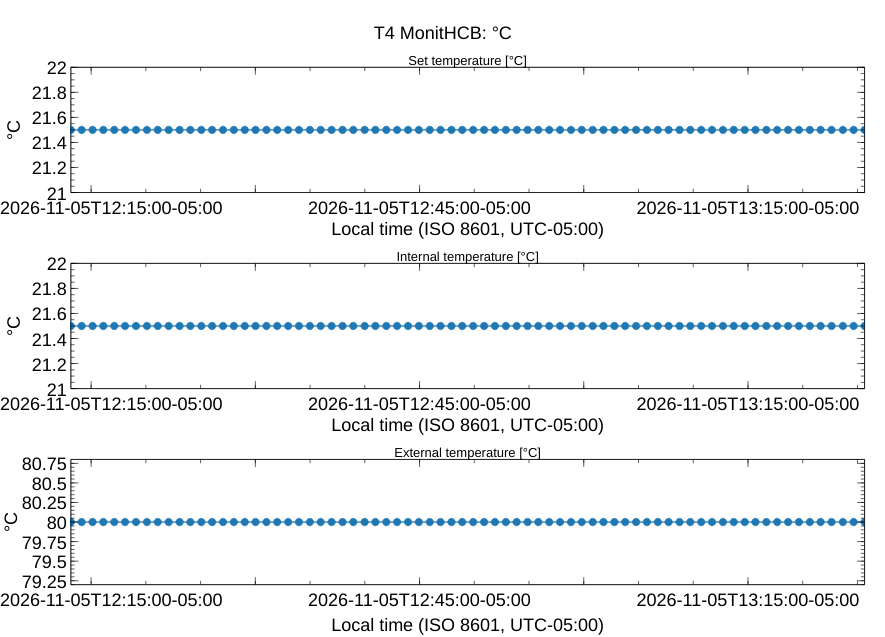
\includegraphics[width=.7\linewidth]{../validation/veusz_render_v0.2.1/t4_telemetry_p01_t4log0_monithcb_unit0_local.png}
\end{cfigure}
\warning{The format is inferred from one HCB file. The main 40-channel monitoring file has not been
seen; the reader is header-driven and should read it if it has the same layout, but this is
untested. HCB alarm codes are not documented here.}

\section{Operator script: tools/T4\_Reboot.py}
The workbench sends no settings and no REBOOT. \texttt{tools/T4\_Reboot.py} 0.0.4 is a separate
operator script that reboots the M\&C software after checks; it is untested on a real T4.
\begin{enumerate}[leftmargin=6mm]
\item Read-only checks \texttt{GETID;}, \texttt{RDFS;}, \texttt{RDREG=DRIFTCOMP;} from local port
14000. Each answer must start with \texttt{\$} and the command; \texttt{!<command>} is a rejection
(\tfournet, Sec.~1.1.2, p.~11). Any failure stops the script before REBOOT.
\item The operator types \texttt{REBOOT}; the command is sent once. Table~1 lists no answer, so
silence is the expected result; \texttt{!REBOOT} stops the script.
\item After 30~s (the manual's wait after a front-panel reset, Sec.~6.7, p.~24; none is given for
REBOOT) the checks are repeated and compared. RDFS may change on its own when drift compensation
steps the synthesizer.
\end{enumerate}
Exit codes: 0 success or cancelled, 1 pre-check failed (nothing sent), 2 post-check failed,
3 REBOOT rejected or not sent. The original 0.0.1 script waited for a reply to REBOOT and therefore
ended with \texttt{TimeoutError} even when the reboot worked (reproduced on loopback). Sec.~1.1.3
(p.~13) describes REBOOT as ``Reset the LAN module'' and Sec.~6.7 (p.~24) says the equivalent
telnet reset ``will not affect the stability or the 1PPS generation''; confirm 1~PPS after a reboot.
\clearpage
\section{Stability analysis and Stable32 (base tab)}\label{sec:stability}
\subsection{What the base Stability tab computes}
OADEV, MDEV, TDEV and OHDEV use phase samples in seconds and the NIST SP 1065
definitions \nist, equations (A25)--(A28) of Appendix A. The calculation supports raw phase, mean
removal, linear phase removal and quadratic phase removal. Results are labeled with the chosen
detrending; raw stability must not be confused with fitted-residual stability. The traces are
described in Appendix C.

The code validates both adjacent intervals and cumulative deviation from a uniform grid, equations
(A22)--(A23). It never fills gaps or interpolates samples. The mean actual interval establishes the
nominal sampling period after validating the record. The default relative tolerance is 1\%; the
interface allows up to 5\%. This is an explicit approximate-uniformity tolerance, not proof that
jitter has no effect at the shortest averaging times.

For the supplied month, a 2\% tolerance admits an approximately 3 s maximum
grid deviation on a 270 s cadence. The default 1\% rejects the full record.
An internal exclusion creates a missing interval and is not compressed away
to make a false uniform series; such a record is refused here and can be analysed in the
gap-aware evaluation tab instead (section ``\nameref{sec:gapstab}'').

At least ten contributing terms are required for each plotted estimate.
Overlapping terms are correlated; their count is not an equivalent number of
independent degrees of freedom. The base tab shows no confidence bands and claims no maser-only
noise separation \nist; the evaluation tabs add both (confidence intervals; three-cornered hat).

\subsection{Which data the stability describes}
The stability is computed from the \emph{timing phase}: the measured 1 PPS time difference between
the maser and the reference (GPS). It is therefore the stability of the comparison (maser, GPS
receiver and link, counter and cables), not of the maser alone. The HMD and T4 telemetry are
housekeeping (temperatures, voltages, synthesizer settings); they are not a frequency measurement and
cannot give a frequency stability by themselves. Release 0.3.0 uses the HMD only to remove the
steering that the maser's own synthesizer applied (section ``\nameref{sec:steering}''). A gap-skipping
OADEV of the 193-day Franks MSM-GPS record gives \(6.3\times10^{-13}\) at 1~h, \(6.1\times10^{-14}\)
at 1~d and \(1.7\times10^{-14}\) at 1~week, while the MHM~2010 datasheet gives
\(1.5\times10^{-15}\) at \(10^4\)~s and a floor below \(1\times10^{-15}\) \mhmdata: the curve measures
the GPS comparison out to about two weeks and is only an upper bound on the maser.

\begin{cfigure}{Base Stability tab: OADEV, MDEV, OHDEV (upper) and TDEV (lower) of the selected samples.\label{fig:guistab}}
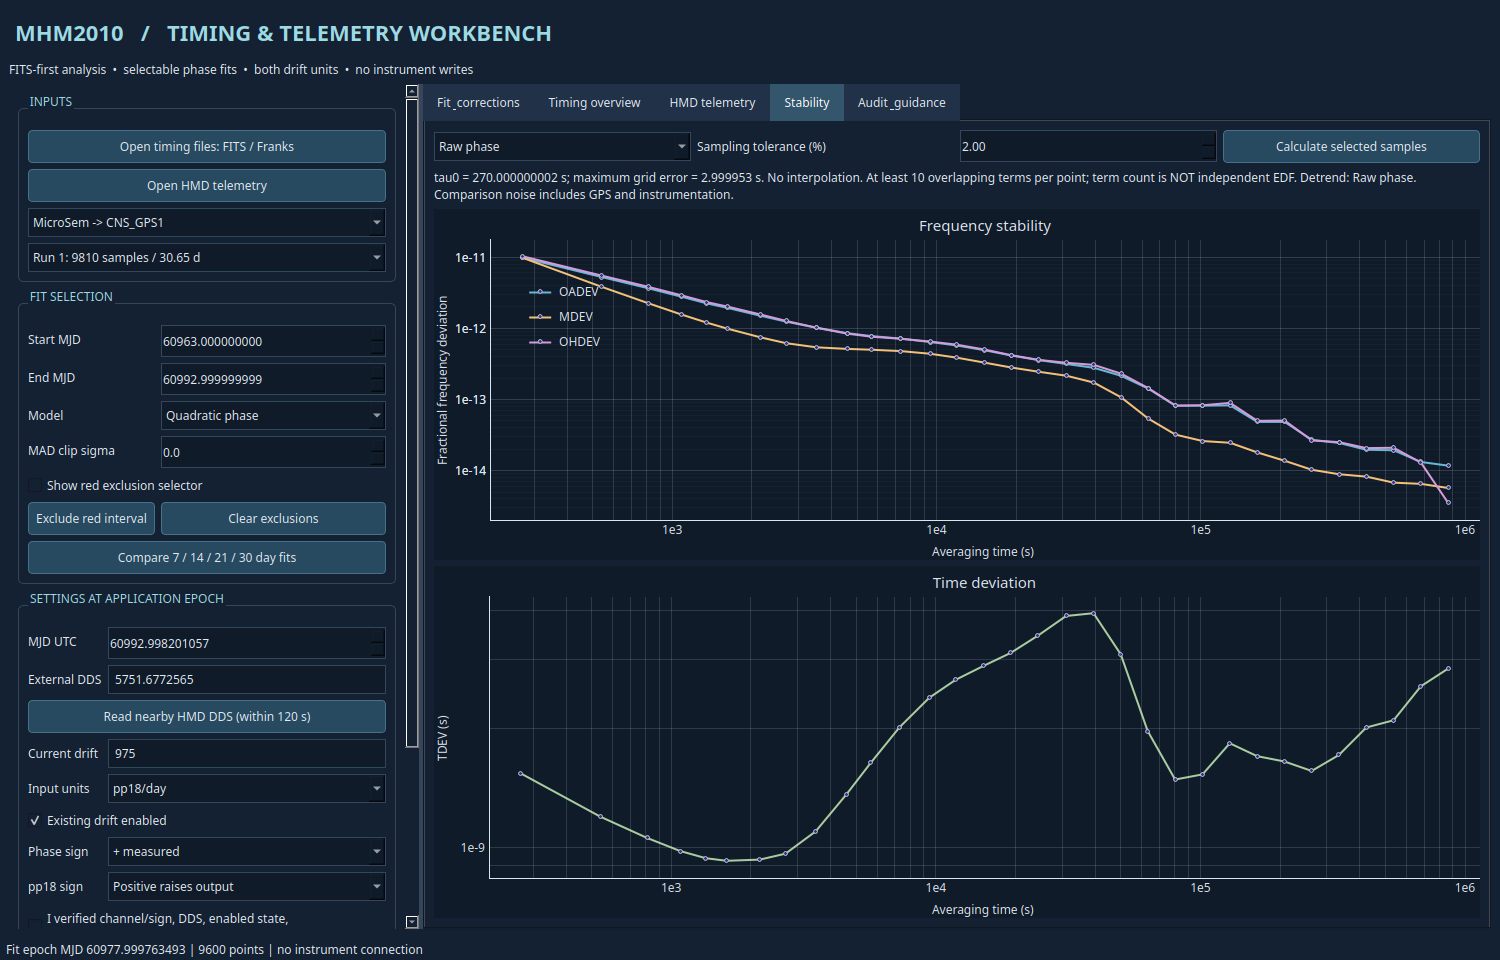
\includegraphics[width=.94\linewidth]{../validation/gui_stability.png}
\end{cfigure}

\subsection{Stable32 files}
\texttt{raw.PHD} holds phase seconds and \texttt{raw.FRD} holds fractional
frequency derived from successive phase samples, equation (A24). The frequency record has one
fewer point. Fit-residual versions are written separately. The headers contain
type, point count and tau; companion CSV/JSON files retain original timestamps,
units, tolerance checks and export decisions \stablemanual.

Stable32 treats embedded zeros as gaps. Actual zeros are exported as
\texttt{1e-99}, following the manual's recommendation; replacements are counted
in the sidecar \stablemanual. Do not use its gap-fill controls to disguise a
nonuniform or incomplete input record.
\clearpage

\section{Further evaluation (release 0.3.0)}\label{sec:evaluation}
\subsection{Principles}
Four tabs, placed after ``Stability'' and before ``Audit \& guidance'', evaluate the same data in
other ways. Each tab has a banner, a row of controls, a \textbf{Calculate} button, plots and a
read-only text pane with every number. The \textbf{Evaluate} menu has one entry per tab (``Calculate
gap-aware stability'', ``Calculate steering removal'', ``Calculate Kalman estimate'', ``Calculate
three-cornered hat'') and ``Tick every evaluation page for export''.
\begin{itemize}
\item \textbf{Evaluation only.} The tabs read the loaded data, the fit interval, the base fit, the
application epoch, the phase sign and the maser selection; they write nothing back. The base fit, the
Results box, the suggested settings and the reference figures are unchanged (tested). Settings derived
from the Kalman estimate are labelled EVALUATION ONLY and appear only in that tab, its pages and its
JSON entry.
\item \textbf{No filled data.} Following NIST SP 1065 \nist, a gap stays a gap. For the Allan
variance SP 1065 says that a pair touching a gap ``is skipped in the summation'' (Sec.~10.4); it
allows interpolation for analyses that cannot skip, and warns that with many gaps ``the results will be
suspect'' (Sec.~10.6). The workbench skips; it never interpolates. The Kalman filter crosses a gap by
prediction alone, so its uncertainty grows there. The grid and gap counts are reported with every
result.
\item \textbf{Shared code.} The GUI tabs and \texttt{analyze\_maser.py} call the same runners in
\texttt{maser\_eval.py}, so a batch result equals the tab result for the same options.
\item \textbf{Parallel work.} Averaging factors (and the three pairs of the hat) run in a thread pool;
NumPy releases the interpreter lock in the vector operations. The arrays are small (at most about
\(10^5\) samples), so the GPU is not used: the transfer would cost more than the work.
\end{itemize}

\begin{ctable}{The four evaluation tabs: data, method and output\label{tab:evaltabs}}
\begin{tabular}{@{}P{.18\linewidth}P{.25\linewidth}P{.27\linewidth}P{.22\linewidth}@{}}
\toprule
Tab & Data used & Method & Veusz pages / file\\
\midrule
Eval: gap-aware stability & selected samples of the base fit, or the steering-removed samples &
grid with gap markers; OADEV, MDEV, TDEV, OHDEV skipping gap terms; lag-1 noise type; confidence
intervals & \texttt{GapStab\_*}; \texttt{evaluation\_gap\_stability.csv}\\
Eval: steering removal & whole selected channel and the HMD DDS column & DDS to fractional frequency,
integrated to phase, removed; same fit of the removed record & \texttt{Steer\_*};
\texttt{evaluation\_steering\_removed.csv}\\
Eval: Kalman estimate & samples used in the base fit & three-state clock model, Kalman filter and RTS
smoother; noise from the gap-aware OHDEV & \texttt{Kalman\_*}; \texttt{evaluation\_kalman.csv}\\
Eval: three-cornered hat & three loaded channels, or two against a common clock &
pair OADEVs on common time stamps; Gray--Allan separation & \texttt{TCH\_allan\_deviation};
\texttt{evaluation\_three\_cornered\_hat.csv}\\
\bottomrule
\end{tabular}
\end{ctable}

% ---------------------------------------------------------------------------
\subsection{Eval: gap-aware stability}\label{sec:gapstab}
\textbf{Purpose.} The base Stability tab refuses a record with gaps or uneven spacing. This tab
places the samples on a regular grid, marks empty slots as gaps, computes the four estimators from
the terms whose samples all exist, identifies the dominant noise type and gives confidence intervals
\nist, \sesia, \lagone. On a gap-free uniform record its deviations equal the base tab (tested to
\(10^{-12}\) relative) and AllanTools \allantools.

\begin{ctable}{Controls of the tab ``Eval: gap-aware stability'' and their batch equivalents\label{tab:gapcontrols}}
\begin{tabular}{@{}P{.15\linewidth}P{.33\linewidth}P{.21\linewidth}P{.23\linewidth}@{}}
\toprule
Control & Choices (default first) & Batch flag & Meaning\\
\midrule
Detrend & Raw phase; Remove mean; Remove linear phase; Remove quadratic phase & \texttt{--gap-detrend -1|0|1|2} &
polynomial removed before the estimators (G5)\\
Grid & Auto; Anchored (fixed clock); Sequential (own intervals) & \texttt{--gap-grid auto|\allowbreak anchored|\allowbreak sequential} &
how samples are placed in slots (G2--G4)\\
tau0 & auto (median interval) or a value in s & \texttt{--gap-tau0 S} & grid step \(\tau_0\) (G1)\\
Slot tolerance & 10\,\% of \(\tau_0\) (1--50\,\%) & \texttt{--gap-tolerance 0.10} & \(\kappa\), largest offset placed\\
Confidence & 68.27\,\% (1 sigma); 90\,\%; 95\,\% & \texttt{--confidence L} & level \(L\) of the intervals (X2, X3)\\
Data & Selected samples (as the base fit); Steering-removed samples & \texttt{--gap-source selected|steering-removed} &
the second needs the steering removal\\
\bottomrule
\end{tabular}
\end{ctable}

\textbf{Plots.} ``Gap-aware frequency stability with confidence intervals'' (OADEV, MDEV, OHDEV,
log--log, each point with its interval as an error bar) and ``Gap-aware time deviation'' (TDEV with
its interval). The text pane lists the grid (mode, \(\tau_0\), samples placed, slots, gap slots, gap
runs and the longest, duplicates, largest offset), then one row per estimator and \(\tau\): deviation,
low and high limits, interval method, EDF, noise type and term count.

\subsubsection{Regular grid with gap markers}
\begin{vartable}{tab:var-G}{Variables of the regular grid (G1--G5)}
\(t_i\) & time stamp of input sample \(i\), elapsed SI seconds from the grid origin (TAI difference, as (A1)) & s\\
\(t_o\) & grid origin: the first valid sample & s\\
\(x_i\) & phase of sample \(i\) (maser channel as measured) & s\\
\(\tau_0\) & grid step; default the median positive interval & s\\
\(\kappa\) & slot tolerance, fraction of \(\tau_0\), \(0<\kappa\le0.5\) (default 0.10) & 1\\
\(k\), \(k_i\) & slot index; slot of sample \(i\) & 1\\
\(\phi_i\) & offset of sample \(i\) from its slot time (anchored grid) & \(\tau_0\)\\
\(i'\) & the previously placed sample (sequential grid) & --\\
\(n_i\), \(\mu_i\) & slot advance from \(i'\); its misfit (sequential grid) & slots; \(\tau_0\)\\
\(X_k\) & grid phase in slot \(k\); empty slot = gap (NaN) & s\\
\(N_{\mathrm{in}}\), \(N_{\mathrm{pl}}\), \(N_{\mathrm{sl}}\) & valid input samples; placed samples; number of slots & 1\\
\(p_d\) & detrend order: \(-1\) raw, 0 mean, 1 linear, 2 quadratic & 1\\
\(P_{p_d}(t)\) & OLS polynomial of order \(p_d\) fitted to the placed samples against their real times & s\\
\(k_1\) & first slot holding a sample & 1\\
\end{vartable}
\begin{align}
\tau_0&=\operatorname{median}\{t_{i+1}-t_i>0\}\ \text{(unless given)}, \tag{G1}\label{eq:G1}\\
\text{anchored:}\quad k_i&=\operatorname{round}\frac{t_i-t_o}{\tau_0},\quad
\phi_i=\frac{t_i-t_o}{\tau_0}-k_i,\quad \text{placed if } |\phi_i|\le\kappa,\quad
X_k=x_{\arg\min_{i:k_i=k}|\phi_i|}, \tag{G2}\label{eq:G2}\\
\text{sequential:}\quad n_i&=\operatorname{round}\frac{t_i-t_{i'}}{\tau_0},\quad
k_i=k_{i'}+n_i\ \text{if}\ n_i\ge1\ \text{(else not placed)},\quad
\mu_i=\frac{t_i-t_{i'}}{\tau_0}-n_i, \tag{G3}\label{eq:G3}\\
\text{auto:}\quad &\text{anchored if } N_{\mathrm{pl}}^{\mathrm{anchored}}\ge0.9\,N_{\mathrm{in}},\ \text{otherwise sequential}, \tag{G4}\label{eq:G4}\\
\text{detrend:}\quad X_k&\leftarrow X_k-P_{p_d}(t_{i(k)})\ \ (p_d\ge0),\qquad
X_k\leftarrow X_k-X_{k_1}\ \ (p_d=-1). \tag{G5}\label{eq:G5}
\end{align}
The anchored grid suits a stable sampling clock (FITS, 270~s); of two samples in one slot the closer
is kept and the other counted as a duplicate; samples farther than \(\kappa\tau_0\) from a slot are
counted as off-grid and not placed. The sequential grid follows SP 1065 Secs.~5.16 and 10.5 \nist\ for
jittered data such as Franks hourly medians: each sample advances by the rounded number of steps from the
previous one, so jitter does not accumulate; an interval of \(n_i>1\) steps leaves \(n_i-1\) gap slots;
SP 1065 notes that ``tau variations of \(\pm10\)\,\% will yield reasonable results''; intervals with
\(|\mu_i|>\kappa\) are counted and reported, not rejected. Values are never moved or interpolated; only
their slot is chosen. A raw record has a constant removed, which does not change any estimator.

\subsubsection{Estimators that skip gaps}
\begin{vartable}{tab:var-H}{Variables of the gap-aware estimators (H1--H4)}
\(m\) & averaging factor (integer) & 1\\
\(\tau\) & averaging time \(m\tau_0\) & s\\
\(\Delta^2_k\) & second difference \(X_{k+2m}-2X_{k+m}+X_k\) & s\\
\(\Delta^3_k\) & third difference \(X_{k+3m}-3X_{k+2m}+3X_{k+m}-X_k\) & s\\
\(S_j\) & sum of \(m\) consecutive second differences, \(\sum_{k=j}^{j+m-1}\Delta^2_k\) & s\\
\(\mathcal V_2\), \(\mathcal V_3\) & slots whose second (third) difference has all its samples & --\\
\(\mathcal V_M\) & start slots whose \(m\) second differences all exist & --\\
\(T_2\), \(T_3\), \(T_M\) & term counts \(|\mathcal V_2|\), \(|\mathcal V_3|\), \(|\mathcal V_M|\) (at least 10) & 1\\
\(\sigma_y(\tau)\) & overlapping Allan deviation (OADEV) & 1\\
\(\operatorname{mod}\sigma_y(\tau)\) & modified Allan deviation (MDEV) & 1\\
\(\sigma_x(\tau)\) & time deviation (TDEV) & s\\
\(\sigma_H(\tau)\) & overlapping Hadamard deviation (OHDEV) & 1\\
\end{vartable}
\begin{align}
\sigma_y^2(\tau)&=\frac{1}{2\tau^2T_2}\sum_{k\in\mathcal V_2}\bigl(\Delta^2_k\bigr)^2, \tag{H1}\label{eq:H1}\\
\operatorname{mod}\sigma_y^2(\tau)&=\frac{1}{2m^2\tau^2T_M}\sum_{j\in\mathcal V_M}S_j^2, \tag{H2}\label{eq:H2}\\
\sigma_x(\tau)&=\frac{\tau}{\sqrt3}\operatorname{mod}\sigma_y(\tau), \tag{H3}\label{eq:H3}\\
\sigma_H^2(\tau)&=\frac{1}{6\tau^2T_3}\sum_{k\in\mathcal V_3}\bigl(\Delta^3_k\bigr)^2. \tag{H4}\label{eq:H4}
\end{align}
Without gaps, \(T_2=N_{\mathrm{sl}}-2m\), \(T_M=N_{\mathrm{sl}}-3m+1\) and \(T_3=N_{\mathrm{sl}}-3m\), and
(H1)--(H4) are (A25)--(A28). The averaging factors are the base tab's: 35 log-spaced integers from 1
to \(\max\bigl(1,\lfloor(N_{\mathrm{sl}}-10)/3\rfloor\bigr)\), duplicates removed; a point needs at least
ten terms. Skipping terms that touch a gap is the SP 1065 rule for the Allan variance \nist\ and the
approach studied by Sesia and Tavella for long periods of missing data \sesia; the reported term counts
show how much of the record each point uses.

\subsubsection{Noise identification (lag-1 autocorrelation)}
\begin{vartable}{tab:var-N}{Variables of the lag-1 noise identification (N1--N3)}
\(\xi_j\) & longest gap-free run of the grid, decimated by \(m\), a quadratic removed, then differenced \(d\) times & s\\
\(\bar\xi\) & mean of \(\xi_j\) & s\\
\(r_1\) & lag-1 autocorrelation of \(\xi_j\) & 1\\
\(\delta\) & \(r_1/(1+r_1)\) & 1\\
\(d\), \(d_{\max}\) & number of differences; its limit (2 for OADEV, MDEV, TDEV; 3 for OHDEV) & 1\\
\(\hat\alpha\), \(\alpha\) & estimated and rounded power-law exponent, \(S_y(f)\propto f^{\alpha}\) & 1\\
\(S_y(f)\) & one-sided spectral density of fractional frequency & Hz\(^{-1}\)\\
\end{vartable}
\begin{align}
r_1&=\frac{\sum_j(\xi_j-\bar\xi)(\xi_{j+1}-\bar\xi)}{\sum_j(\xi_j-\bar\xi)^2},\qquad
\delta=\frac{r_1}{1+r_1}, \tag{N1}\label{eq:N1}\\
&\text{difference again while } \delta\ge0.25 \text{ and } d<d_{\max}, \tag{N2}\label{eq:N2}\\
\hat\alpha&=2-2(\delta+d),\qquad
\alpha=\operatorname{clip}\bigl(2-\operatorname{round}(2\delta)-2d,\,-2,\,2\bigr). \tag{N3}\label{eq:N3}
\end{align}
\(\alpha=2,1,0,-1,-2\) is white PM, flicker PM, white FM, flicker FM and random-walk FM. The method is
that of Riley and Greenhall \lagone, SP 1065 Secs.~5.5.4--5.5.5 \nist; at least 30 decimated points are
needed, otherwise the noise type is ``not identified''. It is evaluated on the longest gap-free run, so
gaps never enter the autocorrelation. The same definitions as AllanTools are used (tested: the same noise
type and number of differences).

\subsubsection{Equivalent degrees of freedom and confidence intervals}
\begin{vartable}{tab:var-X}{Variables of the equivalent degrees of freedom and confidence intervals (X1--X3)}
\(N_{\mathrm{eq}}\) & equivalent gap-free number of phase points, \(T_2+2m\) & 1\\
\(m\), \(\alpha\) & averaging factor; identified noise exponent (N3) & 1\\
\(\nu_{\mathrm{edf}}\) & equivalent degrees of freedom of the OADEV estimate & 1\\
\(\hat\sigma\) & estimated deviation (any of H1--H4) & 1 (s for TDEV)\\
\(L\) & confidence level (default \(\operatorname{erf}(1/\sqrt2)=0.6826894921370859\), one standard deviation) & 1\\
\(\beta\) & \(1-L\), the two tails together & 1\\
\(\chi^2_p(\nu)\) & \(p\)-quantile of the chi-squared distribution with \(\nu\) degrees of freedom & 1\\
\(z_L\) & normal quantile \(\Phi^{-1}\bigl((1+L)/2\bigr)\) (1 for one standard deviation) & 1\\
\(T\) & term count of the estimate (\(T_2\), \(T_M\) or \(T_3\)) & 1\\
\(\sigma_{\mathrm{lo}}\), \(\sigma_{\mathrm{hi}}\) & lower and upper confidence limits & as \(\hat\sigma\)\\
\end{vartable}
For OADEV, with \(N=N_{\mathrm{eq}}\), the simple EDF approximations of SP 1065 Table~5 (Sec.~5.4.1)
\nist\ are used:
\begin{equation}
\nu_{\mathrm{edf}}=\begin{cases}
\dfrac{(N+1)(N-2m)}{2(N-m)}, & \alpha=2,\\[8pt]
\exp\sqrt{\ln\dfrac{N-1}{2m}\,\ln\dfrac{(2m+1)(N-1)}{4}}, & \alpha=1,\\[8pt]
\left[\dfrac{3(N-1)}{2m}-\dfrac{2(N-2)}{N}\right]\dfrac{4m^2}{4m^2+5}, & \alpha=0,\\[8pt]
\dfrac{2(N-2)}{2.3N-4.9}\ (m=1),\qquad \dfrac{5N^2}{4m(N+3m)}\ (m\ge2), & \alpha=-1,\\[8pt]
\dfrac{N-2}{m(N-3)^2}\left[(N-1)^2-3m(N-1)+4m^2\right], & \alpha=-2.
\end{cases} \tag{X1}\label{eq:X1}
\end{equation}
The chi-squared interval (SP 1065 Sec.~5.3.2, Eq.~45) and, where no EDF applies, the simple interval
(Sec.~5.3.1) are:
\begin{align}
\sigma_{\mathrm{lo}}&=\hat\sigma\sqrt{\frac{\nu_{\mathrm{edf}}}{\chi^2_{1-\beta/2}(\nu_{\mathrm{edf}})}},\qquad
\sigma_{\mathrm{hi}}=\hat\sigma\sqrt{\frac{\nu_{\mathrm{edf}}}{\chi^2_{\beta/2}(\nu_{\mathrm{edf}})}}
\qquad(\text{OADEV with a noise type}), \tag{X2}\label{eq:X2}\\
\sigma_{\mathrm{lo}}&=\max\!\left(0,\ \hat\sigma\Bigl(1-\frac{z_L}{\sqrt T}\Bigr)\right),\qquad
\sigma_{\mathrm{hi}}=\hat\sigma\Bigl(1+\frac{z_L}{\sqrt T}\Bigr)
\qquad(\text{MDEV, TDEV, OHDEV, or no noise type}). \tag{X3}\label{eq:X3}
\end{align}
The method of each point (\texttt{chi2\_simple\_edf} or \texttt{simple\_sigma\_over\_sqrtN}) is written
beside it. The simple interval of (X3) uses the term count, which overstates the independent
information of overlapping terms, so it is narrower than a full EDF interval would be; it is labelled
as such. \(N_{\mathrm{eq}}\) treats a gapped record as if it were gap-free with the same number of
terms, an approximation that SP 1065 does not define for gaps.

% ---------------------------------------------------------------------------
\subsection{Eval: steering removal}\label{sec:steering}
\textbf{Purpose.} The MHM2010 output is steered by its external DDS: manual steps and the drift
compensation, which changes the DDS slowly (in the historical month \texttt{ExtSynth\_32} falls by about
13 counts/day). The HMD records the DDS. This tab converts the recorded DDS to the fractional frequency
it applied, integrates it to phase and removes it from the measured channel, showing the maser without
its recorded steering, then fits the removed record with the base model and window. The constants are
those of the base DDS calculation (A13)--(A14) \manual.

\begin{ctable}{Controls of the tab ``Eval: steering removal'' and their batch equivalents\label{tab:steercontrols}}
\begin{tabular}{@{}P{.15\linewidth}P{.33\linewidth}P{.21\linewidth}P{.23\linewidth}@{}}
\toprule
Control & Choices (default first) & Batch flag & Meaning\\
\midrule
Remove & All DDS changes (steps and drift compensation); Steps only (\(>\) threshold) &
\texttt{--steering-mode all|steps} & which changes are removed (W2)\\
Step threshold & 50 counts & \texttt{--steering-threshold 50} & \(\theta\): a jump between consecutive HMD rows larger than this is a step\\
DDS column & \texttt{ExtSynth\_32}; \texttt{Thumbwheels\_31} & \texttt{--steering-column NAME} & HMD column with the DDS that drives the output\\
(phase sign) & the side panel's phase sign & \texttt{--phase-sign} & \(\epsilon\) in (W4)\\
(enable) & Calculate, or the export checkbox & \texttt{--remove-steering} (needs \texttt{--hmd}) & --\\
\bottomrule
\end{tabular}
\end{ctable}

\textbf{Plots.} ``Measured and steering-removed phase'' (Measured, Steering removed, and Fit of removed
record, against time) and ``Recorded steering: applied fractional frequency'' (from the HMD column).
The text pane gives the reference DDS, the HMD rows, the covered samples, the step events, the held
HMD intervals and a table of the base fit and the steering-removed fit at the application epoch.

\begin{vartable}{tab:var-W}{Variables of the steering removal (W1--W4)}
\(j\), \(T_j\) & HMD row index; its time (elapsed SI seconds) & 1; s\\
\(N_j\) & DDS of HMD row \(j\) (column \texttt{ExtSynth\_32} by default) & DDS units\\
\(N_j^{\mathrm{used}}\) & DDS used for row \(j\) (all changes, or steps only) & DDS units\\
\(N_{\mathrm{ref}}\) & reference DDS: the value used at the first covered timing sample & DDS units\\
\(a\), \(q\) & \(2\times10^{-7}\); one count \(10^{-7}\) & 1; DDS units\\
\(\theta\) & step threshold & counts\\
\(\mathbf 1[\cdot]\) & indicator, 1 when the condition holds & 1\\
\(\Delta y_j\) & output fractional frequency applied by \(N_j^{\mathrm{used}}\) relative to \(N_{\mathrm{ref}}\) & 1\\
\(\Psi(t)\) & applied phase, the integral of \(\Delta y\) with zero-order hold & s\\
\(t_i\), \(t_{\mathrm{first}}\) & timing sample time; first timing sample inside the HMD record & s\\
\(x(t_i)\) & measured phase of the channel & s\\
\(x^{\mathrm{rem}}(t_i)\) & phase with the recorded steering removed & s\\
\(\epsilon\) & phase sign, \(\pm1\) (\(\epsilon x\) = maser minus reference) & 1\\
\end{vartable}
\begin{align}
\Delta y_j&=\frac{D(N_{\mathrm{ref}})}{D(N_j^{\mathrm{used}})}-1
=\frac{a\,(N_{\mathrm{ref}}-N_j^{\mathrm{used}})}{284.08+a\,N_j^{\mathrm{used}}},\qquad D(N)=284.08+aN, \tag{W1}\label{eq:W1}\\
N_j^{\mathrm{used}}&=\begin{cases}N_j & \text{all changes},\\[2pt]
N_0+\sum_{l=1}^{j}(N_l-N_{l-1})\,\mathbf 1\!\left[\,|N_l-N_{l-1}|/q>\theta\,\right] & \text{steps only},\end{cases} \tag{W2}\label{eq:W2}\\
\Psi(t)&=\sum_{l<j}\Delta y_l\,(T_{l+1}-T_l)+\Delta y_j\,(t-T_j),\quad T_j\le t<T_{j+1};\qquad
\Psi(t)\leftarrow\Psi(t)-\Psi(t_{\mathrm{first}}), \tag{W3}\label{eq:W3}\\
x^{\mathrm{rem}}(t_i)&=x(t_i)-\epsilon\,\Psi(t_i)\qquad (T_0\le t_i\le T_{\mathrm{last}};\ \text{otherwise not corrected}). \tag{W4}\label{eq:W4}
\end{align}
Raising the DDS lowers the output (W1), as in (A14). Between HMD rows the DDS is held (zero-order
hold); holds longer than 1~h are listed, because a change inside one would be misplaced in time.
Timing samples outside the HMD record are not corrected and are left out of the removed record. The
removed record is fitted with the base model order and window (gap bridging as the base), and the
frequency and drift at the application epoch are compared with the base fit (S1). The tab notes that the
selector codes \texttt{IntExtSwitch\_33} and \texttt{IntExtSoft\_34} are not decoded: confirm that the
external DDS drives the output. An HMD record that does not overlap the timing data is refused with the
two MJD ranges.

% ---------------------------------------------------------------------------
\subsection{Eval: Kalman estimate}\label{sec:kalman}
\textbf{Purpose.} The base fit assumes one polynomial with independent (white) residuals over the
window. The Kalman estimate models the comparison as a clock whose frequency and drift may wander,
with the noise levels taken from the data, and gives the frequency and drift at every sample and at the
application epoch with uncertainties that reflect the identified noise \galleani, \zucca. It is shown
beside the base least-squares values and never replaces them.

\begin{ctable}{Controls of the tab ``Eval: Kalman estimate'' and their batch equivalents\label{tab:kalmancontrols}}
\begin{tabular}{@{}P{.15\linewidth}P{.33\linewidth}P{.21\linewidth}P{.23\linewidth}@{}}
\toprule
Control & Choices (default first) & Batch flag & Meaning\\
\midrule
Noise & Auto: fit to gap-aware OHDEV; Manual values below & \texttt{--kalman-noise R Q1 Q2 Q3} (manual) &
how \(R,q_1,q_2,q_3\) are set (K7, K8)\\
R (s\(^2\)) & manual default \(4\times10^{-18}\) & first value & white PM measurement variance\\
q1 (s) & manual default \(1\times10^{-24}\) & second value & white FM diffusion, \(\sigma_y^2=q_1/\tau\)\\
q2 (1/s) & manual default \(1\times10^{-32}\) & third value & random-walk FM diffusion, \(\sigma_y^2=q_2\tau/3\)\\
q3 (1/s\(^3\)) & manual default 0 & fourth value & random-walk drift diffusion\\
RTS smoothing (plots) & on & \texttt{--no-kalman-smoothing} turns it off & smoothed (K6) or filtered states in the plots\\
\bottomrule
\end{tabular}
\end{ctable}

\textbf{Plots.} ``Kalman fractional frequency (\(\pm1\sigma\)) and base fit'' and ``Kalman drift
(\(\pm1\sigma\)) and base fit'' (the Kalman value with a shaded \(\pm1\sigma\) band and the base
least-squares value dashed), and ``Innovations (measured minus predicted phase)''. The text pane gives
the noise parameters and their source, the OHDEV misfit, the normalized innovation squared, the estimate
at the application epoch beside the base values and, for an eligible maser/reference pair, the settings
from the Kalman estimate marked EVALUATION ONLY.

\begin{vartable}{tab:var-K}{Variables of the Kalman estimate (K1--K9)}
\(k\), \(n\) & sample index; number of samples & 1\\
\(\Delta t_k\) & interval \(d_k-d_{k-1}\) between samples (elapsed SI time) & day\\
\(\mathbf X_k\) & state \((x_k,\dot x_k,\ddot x_k)^{\mathsf T}\): phase, frequency, drift & ns, ns/day, ns/day\(^2\)\\
\(\mathbf F(\Delta t)\) & state transition & --\\
\(\mathbf Q(\Delta t)\) & process-noise covariance of one step & as \(\mathbf X\mathbf X^{\mathsf T}\)\\
\(q_1\), \(q_2\), \(q_3\) & diffusion coefficients: white FM, random-walk FM, random-walk drift & s; s\(^{-1}\); s\(^{-3}\)\\
\(Q_1\), \(Q_2\), \(Q_3\) & the same in the internal units: \(10^{18}\cdot86400\,q_1\), \(10^{18}\cdot86400^3q_2\), \(10^{18}\cdot86400^5q_3\) & ns\(^2\)/day, ns\(^2\)/day\(^3\), ns\(^2\)/day\(^5\)\\
\(R\) & white PM measurement variance (internally \(10^{18}R\) ns\(^2\)) & s\(^2\)\\
\(z_k\) & measured phase & ns\\
\(\mathbf H\) & measurement row \((1,0,0)\) & --\\
\(\hat{\mathbf X}_k^-\), \(\mathbf P_k^-\) & predicted state and covariance & --\\
\(\hat{\mathbf X}_k\), \(\mathbf P_k\) & filtered state and covariance & --\\
\(\nu_k\), \(V_k\) & innovation (measured minus predicted phase); its predicted variance & ns; ns\(^2\)\\
\(\mathbf K_k\) & Kalman gain & --\\
\(\mathbf C_k\) & smoother gain & --\\
\(\hat{\mathbf X}_k^s\), \(\mathbf P_k^s\) & smoothed state and covariance & --\\
\(\tau\), \(\hat\sigma_H^2(\tau_i)\), \(T_{3,i}\) & averaging time; gap-aware OHDEV\(^2\) of the raw phase at \(\tau_i\); its terms & s; 1; 1\\
\(w_i\) & weight \(\sqrt{T_{3,i}}\) & 1\\
NIS & normalized innovation squared & 1\\
\(t_a\), \(t_k\) & application epoch; last sample at or before it & day\\
\(y\), \(r\), \(\sigma_y\), \(\sigma_r\) & frequency and drift at \(t_a\) (\(\epsilon\) applied) and their \(1\sigma\) & 1; day\(^{-1}\)\\
\(\epsilon\) & phase sign & 1\\
\end{vartable}
\begin{align}
\mathbf X_k&=\mathbf F(\Delta t_k)\mathbf X_{k-1}+\mathbf w_k,\qquad
\mathbf F(\Delta t)=\begin{pmatrix}1&\Delta t&\Delta t^2/2\\0&1&\Delta t\\0&0&1\end{pmatrix},\qquad
\mathbf w_k\sim\mathcal N\bigl(0,\mathbf Q(\Delta t_k)\bigr), \tag{K1}\label{eq:K1}\\
\mathbf Q(\Delta t)&=\begin{pmatrix}
Q_1\Delta t+\frac{Q_2\Delta t^3}{3}+\frac{Q_3\Delta t^5}{20} & \frac{Q_2\Delta t^2}{2}+\frac{Q_3\Delta t^4}{8} & \frac{Q_3\Delta t^3}{6}\\[3pt]
\frac{Q_2\Delta t^2}{2}+\frac{Q_3\Delta t^4}{8} & Q_2\Delta t+\frac{Q_3\Delta t^3}{3} & \frac{Q_3\Delta t^2}{2}\\[3pt]
\frac{Q_3\Delta t^3}{6} & \frac{Q_3\Delta t^2}{2} & Q_3\Delta t\end{pmatrix}, \tag{K2}\label{eq:K2}\\
z_k&=\mathbf H\mathbf X_k+v_k,\qquad v_k\sim\mathcal N(0,R), \tag{K3}\label{eq:K3}\\
\hat{\mathbf X}_k^-&=\mathbf F\hat{\mathbf X}_{k-1},\qquad
\mathbf P_k^-=\mathbf F\mathbf P_{k-1}\mathbf F^{\mathsf T}+\mathbf Q, \tag{K4}\label{eq:K4}\\
\nu_k&=z_k-\mathbf H\hat{\mathbf X}_k^-,\quad V_k=\mathbf H\mathbf P_k^-\mathbf H^{\mathsf T}+R,\quad
\mathbf K_k=\frac{\mathbf P_k^-\mathbf H^{\mathsf T}}{V_k},\quad
\hat{\mathbf X}_k=\hat{\mathbf X}_k^-+\mathbf K_k\nu_k, \notag\\
\mathbf P_k&=(\mathbf I-\mathbf K_k\mathbf H)\mathbf P_k^-(\mathbf I-\mathbf K_k\mathbf H)^{\mathsf T}+R\,\mathbf K_k\mathbf K_k^{\mathsf T}, \tag{K5}\label{eq:K5}\\
\mathbf C_k&=\mathbf P_k\mathbf F_{k+1}^{\mathsf T}\bigl(\mathbf P_{k+1}^-\bigr)^{+},\qquad
\hat{\mathbf X}_k^s=\hat{\mathbf X}_k+\mathbf C_k\bigl(\hat{\mathbf X}_{k+1}^s-\hat{\mathbf X}_{k+1}^-\bigr), \notag\\
\mathbf P_k^s&=\mathbf P_k+\mathbf C_k\bigl(\mathbf P_{k+1}^s-\mathbf P_{k+1}^-\bigr)\mathbf C_k^{\mathsf T}, \tag{K6}\label{eq:K6}\\
\sigma_H^2(\tau)&=\frac{10}{3}\frac{R}{\tau^2}+\frac{q_1}{\tau}+\frac{q_2\tau}{6}+\frac{11\,q_3\tau^3}{120}, \tag{K7}\label{eq:K7}\\
(R,q_1,q_2,q_3)&=\arg\min_{\ge0}\sum_i w_i^2\left(\frac{\sigma_H^2(\tau_i)}{\hat\sigma_H^2(\tau_i)}-1\right)^2, \notag\\
\text{misfit}&=\sqrt{\operatorname{mean}_i\left(\frac{\sigma_H^2(\tau_i)}{\hat\sigma_H^2(\tau_i)}-1\right)^2}, \tag{K8}\label{eq:K8}\\
\mathrm{NIS}&=\frac1n\sum_k\frac{\nu_k^2}{V_k};\qquad
y=\frac{\epsilon\,\dot x(t_a)\,10^{-9}}{86400},\quad r=\frac{\epsilon\,\ddot x(t_a)\,10^{-9}}{86400}, \notag\\
\sigma_y&=\frac{\sqrt{P_{22}}\,10^{-9}}{86400},\quad \sigma_r=\frac{\sqrt{P_{33}}\,10^{-9}}{86400}. \tag{K9}\label{eq:K9}
\end{align}
The model is the three-state clock model of Galleani and Tavella \galleani\ and Zucca and Tavella
\zucca; (K2) is its exact discretization. The Hadamard variance of the model (K7) is Eq.~(23b) of
Ishizaki et al. \ishizaki\ (with \(q_i\) there squared) plus the white PM term \((10/3)R/\tau^2\) of a
third difference of independent phase errors; the Hadamard variance is not affected by a constant drift,
so the fit (K8) is made to the gap-aware OHDEV of the raw phase by non-negative least squares, each point
weighted by the square root of its term count. A gap is one longer prediction step: nothing is invented,
and the covariance grows across it. The update uses the Joseph form (K5); the prior is diffuse (the first
measured phase, zero frequency and drift, variances far larger than the data range). The smoother is that of
Rauch, Tung and Striebel \rts\ (K6). The state at the epoch (K9) is the filtered state at the last sample
at or before \(t_a\), predicted forward with (K1)--(K2). NIS (K9) is about 1 when the noise model fits the
data; well above 1 means the model is too confident. For settings (evaluation only), the state at the epoch
is written as a quadratic about the epoch, \(c=(x,\dot x,\ddot x/2)\) at \(d_a=0\), and passed through the
same arithmetic as the base, (S1)--(S4).

% ---------------------------------------------------------------------------
\subsection{Eval: three-cornered hat}\label{sec:tch}
\textbf{Purpose.} A comparison measures two clocks together. With three clocks compared in pairs, the
individual Allan variances follow if the clocks are uncorrelated \grayallan. The tab uses the gap-aware
OADEV (H1) of each pair on their common time stamps.

\begin{ctable}{Controls of the tab ``Eval: three-cornered hat'' and their batch equivalents\label{tab:tchcontrols}}
\begin{tabular}{@{}P{.15\linewidth}P{.33\linewidth}P{.21\linewidth}P{.23\linewidth}@{}}
\toprule
Control & Choices (default first) & Batch flag & Meaning\\
\midrule
Mode & Three measured pairs: A-B, B-C, C-A; Two pairs against a common clock C & \texttt{--tch-mode three|common} & (Q1)\\
Channel A-B, B-C, C-A & loaded channels (A-C and B-C in common mode) & \texttt{--tch CH1 CH2 [CH3]} & which channel compares which clocks (the operator's statement)\\
Clock A/B/C name & A, B, C & \texttt{--tch-names A B C} & labels of the clocks\\
Sign & + measured; - measured (common mode) & \texttt{--tch-signs 1 1} & \(s_1,s_2\): bring the channels to A-C and B-C\\
Detrend each pair & Remove quadratic phase (raw, mean, linear also) & \texttt{--tch-detrend 2} & polynomial removed from each pair\\
\bottomrule
\end{tabular}
\end{ctable}

\textbf{Plot.} ``Three-cornered hat: individual and pair Allan deviations'' (Clock A, B, C solid with
markers; Pair A-B, B-C, C-A dashed). The text pane gives the mode, the common samples, the grid, the
count of non-positive variance estimates per clock, and one row per \(\tau\).

\begin{vartable}{tab:var-Q}{Variables of the three-cornered hat (Q1--Q3)}
A, B, C & the three clocks (names chosen by the operator) & --\\
\(x_1\), \(x_2\), \(x_3\) & phase of the chosen channels on the common time stamps & s\\
\(s_1\), \(s_2\) & signs bringing channels 1 and 2 to A-C and B-C (common mode) & 1\\
\(x_{AB}\), \(x_{BC}\), \(x_{CA}\), \(x_{AC}\) & pair phases & s\\
\(\sigma^2_{AB}(\tau)\), \(\sigma^2_{BC}(\tau)\), \(\sigma^2_{CA}(\tau)\) & gap-aware Allan variance (H1) of each detrended pair & 1\\
\(\sigma^2_A(\tau)\), \(\sigma^2_B(\tau)\), \(\sigma^2_C(\tau)\) & individual Allan variance of each clock & 1\\
\(\sigma_A(\tau)\), \(\sigma_B(\tau)\), \(\sigma_C(\tau)\) & individual Allan deviation (only when the variance is positive) & 1\\
\end{vartable}
\begin{align}
\text{three:}\ \ &x_{AB}=x_1,\ x_{BC}=x_2,\ x_{CA}=x_3, \notag\\
\text{common:}\ \ &x_{AC}=s_1x_1,\ x_{BC}=s_2x_2,\ x_{AB}=s_1x_1-s_2x_2,\ x_{CA}=-s_1x_1, \tag{Q1}\label{eq:Q1}\\
\sigma^2_A&=\tfrac12\left(\sigma^2_{AB}+\sigma^2_{CA}-\sigma^2_{BC}\right),\qquad
\sigma^2_B=\tfrac12\left(\sigma^2_{AB}+\sigma^2_{BC}-\sigma^2_{CA}\right), \notag\\
\sigma^2_C&=\tfrac12\left(\sigma^2_{BC}+\sigma^2_{CA}-\sigma^2_{AB}\right), \tag{Q2}\label{eq:Q2}\\
\sigma_A&=\sqrt{\sigma^2_A}\ \ \text{if}\ \sigma^2_A>0,\ \text{otherwise not shown (the variance is reported)}. \tag{Q3}\label{eq:Q3}
\end{align}
Common time stamps are those equal to \(10^{-7}\)~d (8.64~ms) in every channel; all pairs share one
grid (G1--G4) and one detrend. (Q2) neglects the correlation of the clocks, which Gray and Allan show
does not bias the result when the clocks are independent \grayallan; a negative estimate means the
assumption or the averaging is not sufficient at that \(\tau\). In common mode the pair A-B is
derived, so the measurement noise of both channels enters it, and each channel's measurement noise is
attributed to its own clock. \textbf{Which channel compares which clocks is the operator's statement};
the program cannot know it. If two of the ``clocks'' share a reference (for example two GPS-derived
signals), they are correlated and the separation fails.

% ---------------------------------------------------------------------------
\subsection{Results on the supplied data}\label{sec:evalresults}
The following come from the 0.3.0 export of the historical month (October 15 to November 13, 2025,
MicroSem~\(\rightarrow\)~CNS\_GPS1, quadratic, epoch MJD 60992.998201057395, DDS 5751.6772963) with
every evaluation ticked, and, for the hat, the 2026 Franks files. Every number is the exported value.

\begin{ctable}{Steering removal on the historical month: base fit and steering-removed fit at the application epoch\label{tab:steerresult}}
\begin{tabular}{@{}P{.3\linewidth}P{.31\linewidth}P{.31\linewidth}@{}}
\toprule
Quantity (maser minus reference) & Base fit (measured, steered) & Steering removed (maser alone)\\
\midrule
fractional frequency \(y\) & \(5.838444178725387\times10^{-15}\) & \(-2.2198296389965926\times10^{-14}\)\\
\(1\sigma\) (conditional OLS) & \(2.9491579969249224\times10^{-16}\) & \(2.9508714046127286\times10^{-16}\)\\
drift \(r\) per day & \(-6.60833065550308\times10^{-16}\) & \(-1.5935539121476658\times10^{-15}\)\\
\(1\sigma\) (conditional OLS) & \(1.9038592212810412\times10^{-17}\) & \(1.9049901361802343\times10^{-17}\)\\
samples & 9600 & 9598\\
\bottomrule
\end{tabular}
\end{ctable}
The HMD has 43\,236 rows (MJD 60963.00147 to 60992.997998), no step above 50 counts and no hold above
1~h; 9598 of the 9810 timing samples are covered. The recorded steering ramps the output by
\(2.8020162652892274\times10^{-14}\) over 29.99062499214051~d (a fitted slope of
\(9.331958009774105\times10^{-16}\)/day, \(\approx933\) pp18/day), and the applied phase totals
\(3.639978929902729\times10^{-8}\)~s. \textbf{Cross-check:} the drift difference between the two fits is
\(-9.327208465973579\times10^{-16}\)/day, the recorded ramp to 0.05\,\%, and the frequency difference
\(-2.8036740568691312\times10^{-14}\) is the applied \(2.8020162652892274\times10^{-14}\) to 0.06\,\%.
So in that month the maser itself drifted by about \(-1.59\times10^{-15}\)/day against GPS; the drift
compensation removed about \(9.33\times10^{-16}\)/day of it, and the base suggestion acts on the
remaining \(-6.61\times10^{-16}\)/day. The datasheet's \(<2\times10^{-16}\)/day applies after extended
unperturbed operation \mhmdata.

\begin{ctable}{Gap-aware OADEV of the steering-removed historical month (quadratic removed; anchored grid, \(\tau_0=270.00026993919164\)~s, 9598 slots, no gaps; one-standard-deviation intervals)\label{tab:gapresult}}
\footnotesize
\begin{tabular}{@{}P{.19\linewidth}P{.22\linewidth}P{.3\linewidth}P{.19\linewidth}@{}}
\toprule
\(\tau\) (s) & OADEV & interval (method) & EDF; noise type\\
\midrule
270.00026993919164 & \(9.869169051129275\times10^{-12}\) & \(9.779278428142905\times10^{-12}\) to \(9.961584935814033\times10^{-12}\) (chi2) & 5863.037011054114; flicker PM\\
3510.0035092094913 & \(1.0207102741952156\times10^{-12}\) & \(9.996011867934163\times10^{-13}\) to \(1.0432157340765394\times10^{-12}\) (chi2) & 1097.2309570122752; white FM\\
80190.08017193992 & \(8.157072979077067\times10^{-14}\) & \(7.427862012833443\times10^{-14}\) to \(9.154018112966076\times10^{-14}\) (chi2) & 46.46945520966811; white FM\\
536760.536639113 & \(1.9294871832440765\times10^{-14}\) & \(1.9037538243232353\times10^{-14}\) to \(1.9552205421649177\times10^{-14}\) (simple) & --; not identified\\
\bottomrule
\end{tabular}
\end{ctable}
The record is flicker PM at the shortest averaging time and white FM from about an hour to a day:
at those times the comparison is limited by the GPS link and the 1 PPS measurement, not by the maser
(datasheet \(1.5\times10^{-15}\) at \(10^4\)~s \mhmdata). The interval at the longest \(\tau\) is the
simple one (no noise type with fewer than 30 decimated points) and is too narrow.

\begin{ctable}{Kalman estimate on the historical month (fitted samples; automatic noise) beside the base fit\label{tab:kalmanresult}}
\begin{tabular}{@{}P{.36\linewidth}P{.56\linewidth}@{}}
\toprule
Quantity & Value\\
\midrule
noise (fit to gap-aware OHDEV) & \(R=3.4137902027147988\times10^{-18}\)~s\(^2\), \(q_1=1.9859909536922152\times10^{-22}\)~s, \(q_2=0\), \(q_3=0\)\\
OHDEV misfit (K8); NIS (K9) & 3.3505043228786873; 1.3382282354100896\\
Kalman \(y\) at the epoch & \(-3.3827814393397497\times10^{-15}\pm1.7541716157087668\times10^{-14}\)\\
Kalman \(r\) at the epoch, per day & \(-1.212620617688191\times10^{-15}\pm1.013271635171295\times10^{-15}\)\\
base \(y\); base \(r\) per day & \(5.838444178725387\times10^{-15}\pm2.9491579969249224\times10^{-16}\);
\(-6.60833065550308\times10^{-16}\pm1.9038592212810412\times10^{-17}\)\\
evaluation-only settings & DDS change \(-48.049222131053845\pm249.1635452381788\) counts;
drift change \(+1212.620617688195\pm1013.2716351712985\) pp18/day\\
\bottomrule
\end{tabular}
\end{ctable}
The noise fit keeps white PM and white FM only. With white FM (a random walk of phase) the frequency at
the end of a 30-day window is known to about \(\pm1.75\times10^{-14}\), sixty times the conditional OLS
value, and the drift to about \(\pm1.0\times10^{-15}\)/day, larger than the drift change the base suggests.
This agrees with the window sensitivity of section ``\nameref{sec:historical}'' (the drift changes sign with
the window). The misfit of 3.35 and NIS of 1.34 show that the model does not describe the flicker PM at short
\(\tau\); the uncertainties are indicative.

\begin{ctable}{Three-cornered hat, 2026 Franks files, common mode (MSM-GPS as A-C, CNS\_GPS as B-C; clocks MSM, CNS, GPS; quadratic per pair; sequential grid \(\tau_0=3510.432000271976\)~s, 4643 slots, 4333 placed, 310 gap slots in 17 runs)\label{tab:tchresult}}
\footnotesize
\begin{tabular}{@{}P{.2\linewidth}P{.24\linewidth}P{.24\linewidth}P{.24\linewidth}@{}}
\toprule
\(\tau\) (s) & MSM & CNS & GPS\\
\midrule
3510.432000271976 & \(2.549939126620528\times10^{-13}\) & \(2.5694372621593414\times10^{-13}\) & \(5.793428844083576\times10^{-13}\)\\
87760.8000067994 & \(1.078082531231874\times10^{-14}\) & \(9.87756973943125\times10^{-15}\) & \(5.755705895621374\times10^{-14}\)\\
624856.8960484117 & \(1.7792919617474348\times10^{-15}\) & \(1.101756745065161\times10^{-15}\) & \(1.7960535309336527\times10^{-14}\)\\
\bottomrule
\end{tabular}
\end{ctable}
The GPS term dominates every pair that contains it, as expected. CNS has 7 non-positive variance
estimates. Because the Franks values are hourly medians of 1 PPS comparisons, the MSM and CNS values
include their channels' measurement noise. Whether CNS is independent of GPS (or GPS-derived) is not
known to the program; if it is GPS-derived the separation does not hold.

\begin{cfigure}{GUI tab ``Eval: gap-aware stability'' (Light theme): intervals as error bars.\label{fig:guigap}}
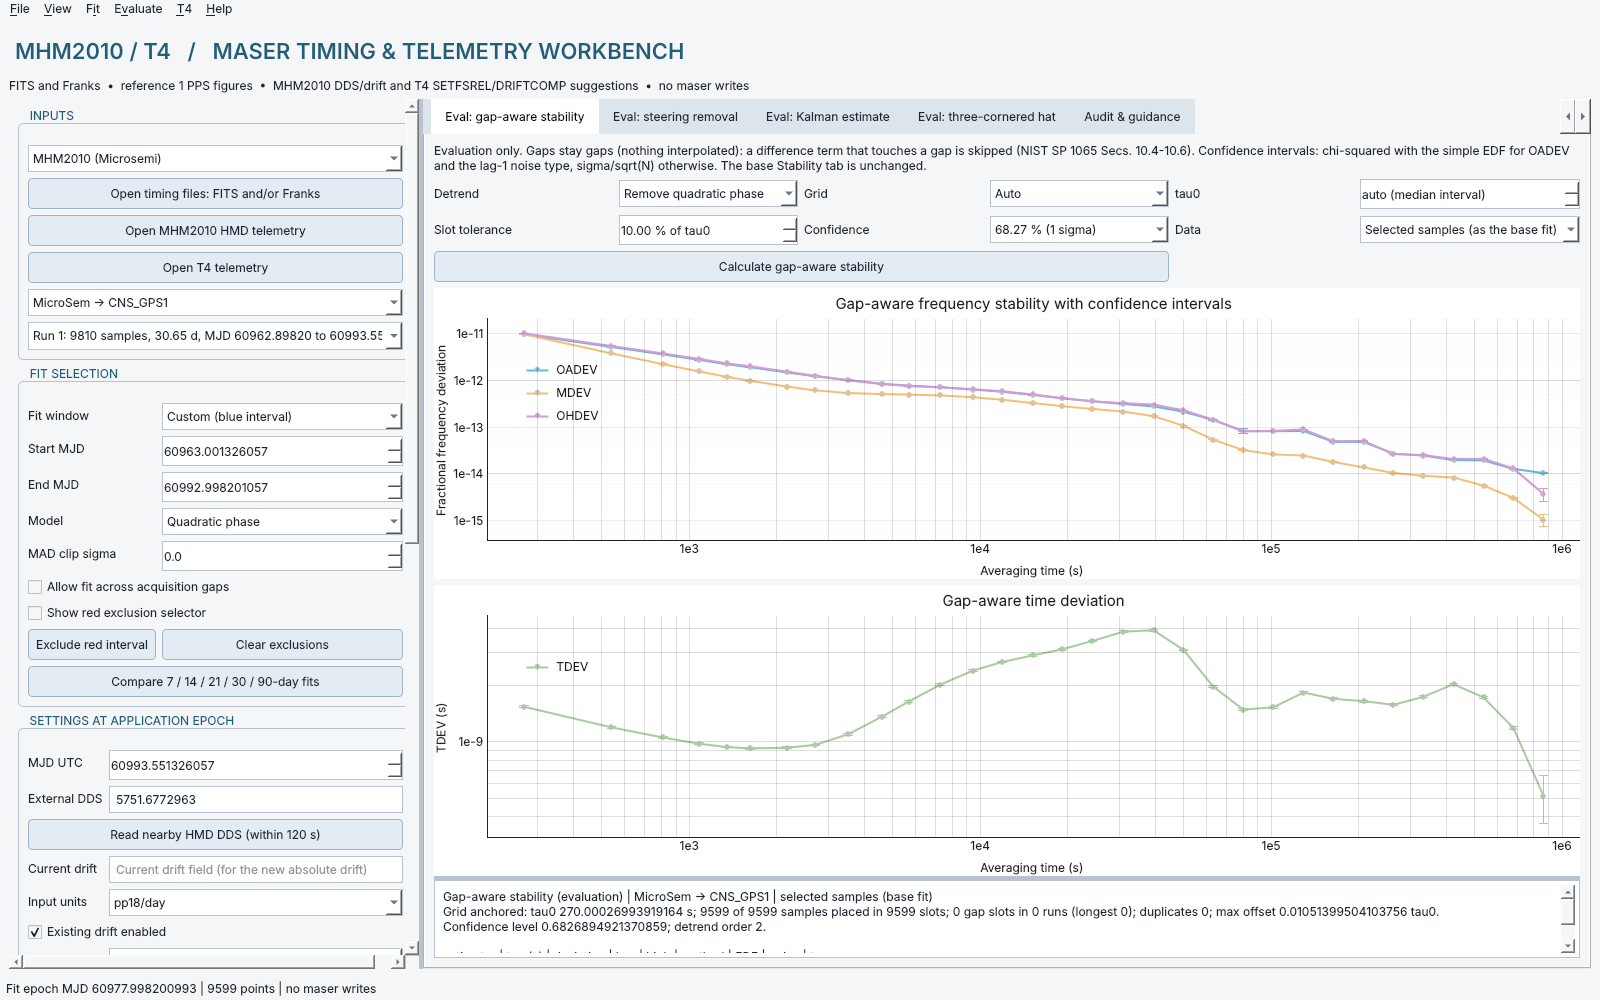
\includegraphics[width=.92\linewidth]{../validation/gui_0.3.0/gui_eval_gap_stability_light.png}
\end{cfigure}
\begin{cfigure}{GUI tab ``Eval: steering removal'' on the historical month.\label{fig:guisteer}}
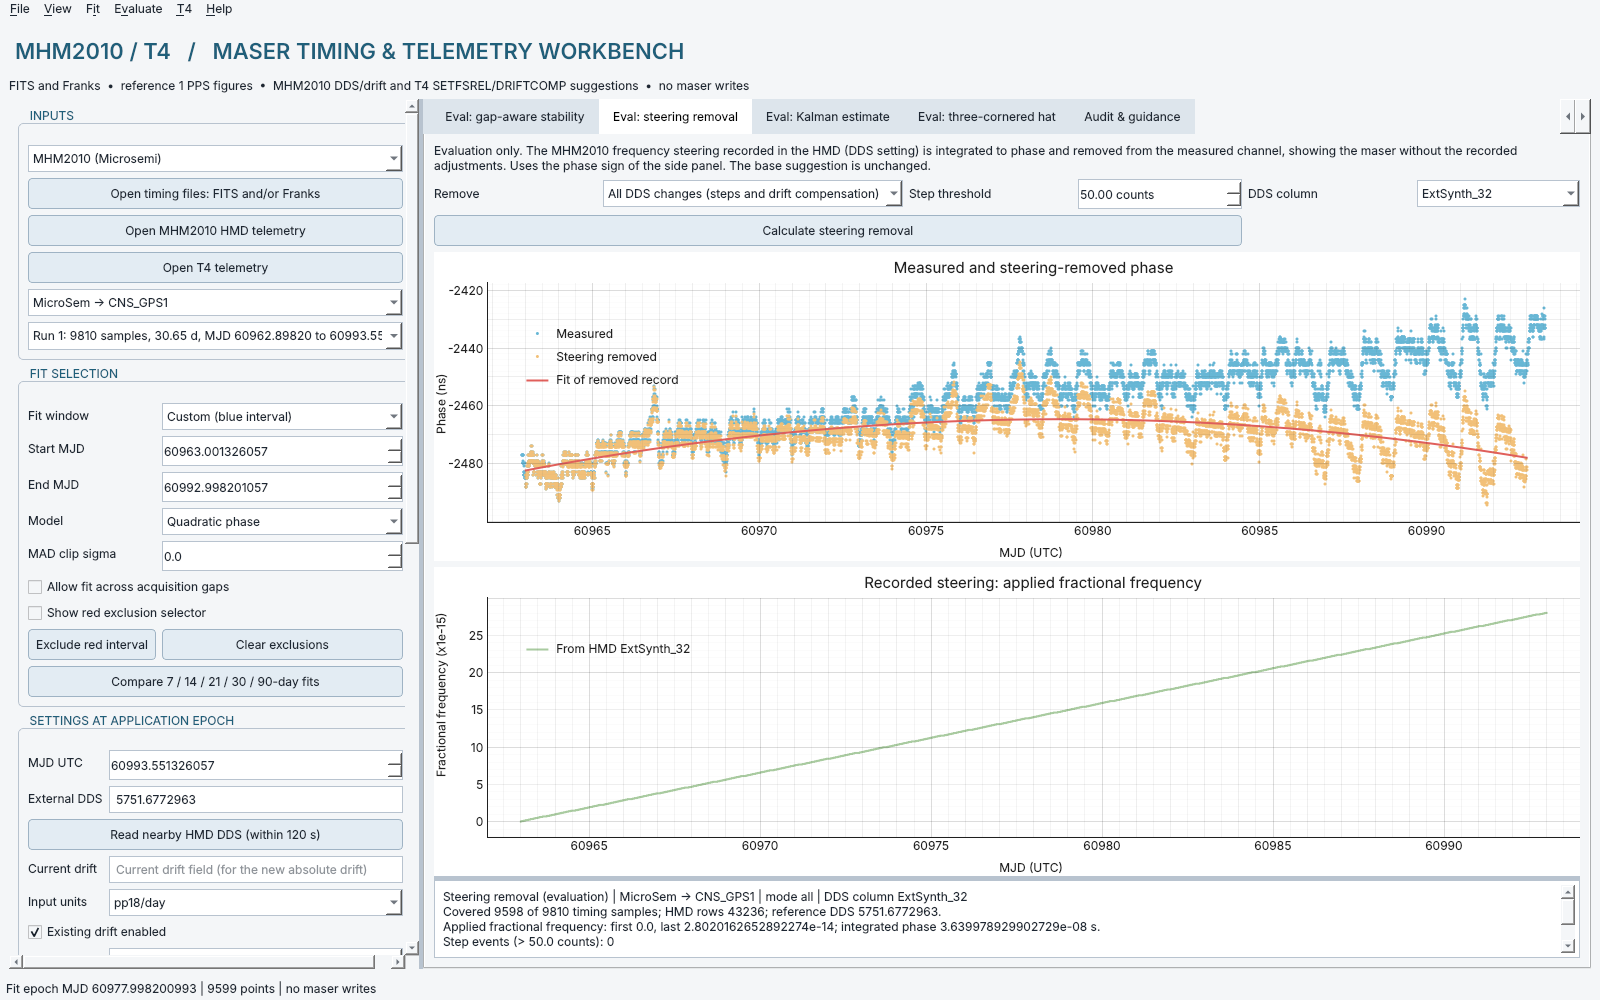
\includegraphics[width=.92\linewidth]{../validation/gui_0.3.0/gui_eval_steering_removal_light.png}
\end{cfigure}
\begin{cfigure}{GUI tab ``Eval: Kalman estimate'' (Light theme): \(\pm1\sigma\) bands, base fit dashed, innovations.\label{fig:guikalman}}
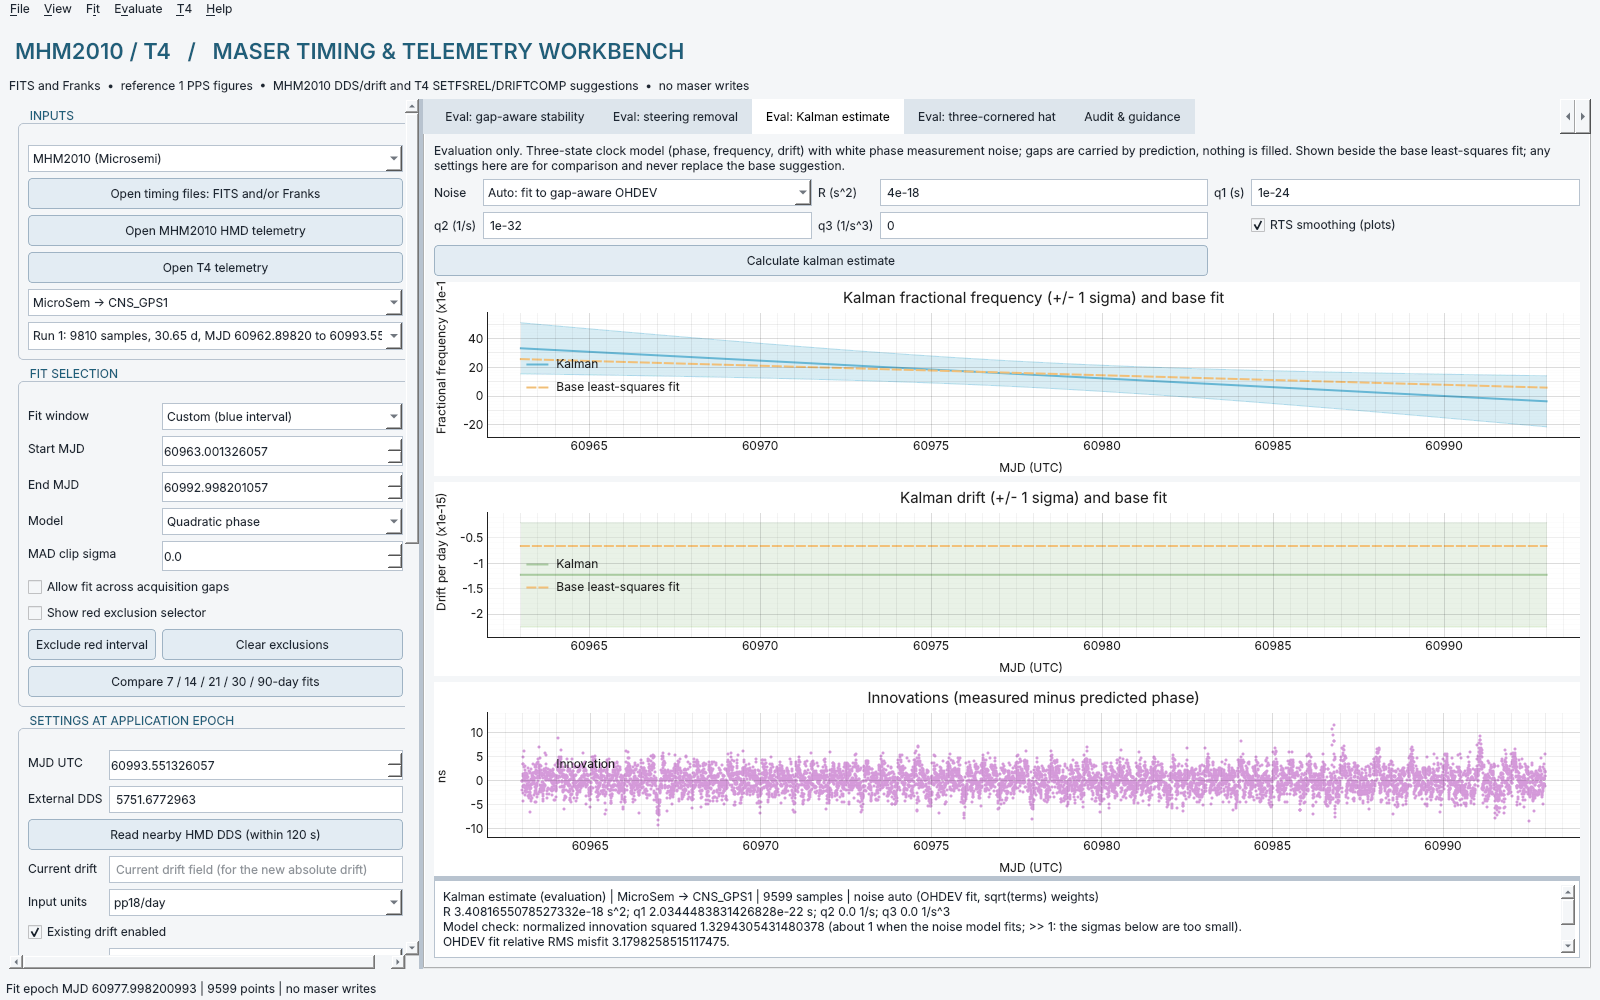
\includegraphics[width=.92\linewidth]{../validation/gui_0.3.0/gui_eval_kalman_light.png}
\end{cfigure}
\begin{cfigure}{GUI tab ``Eval: three-cornered hat'' on the 2026 Franks files.\label{fig:guitch}}
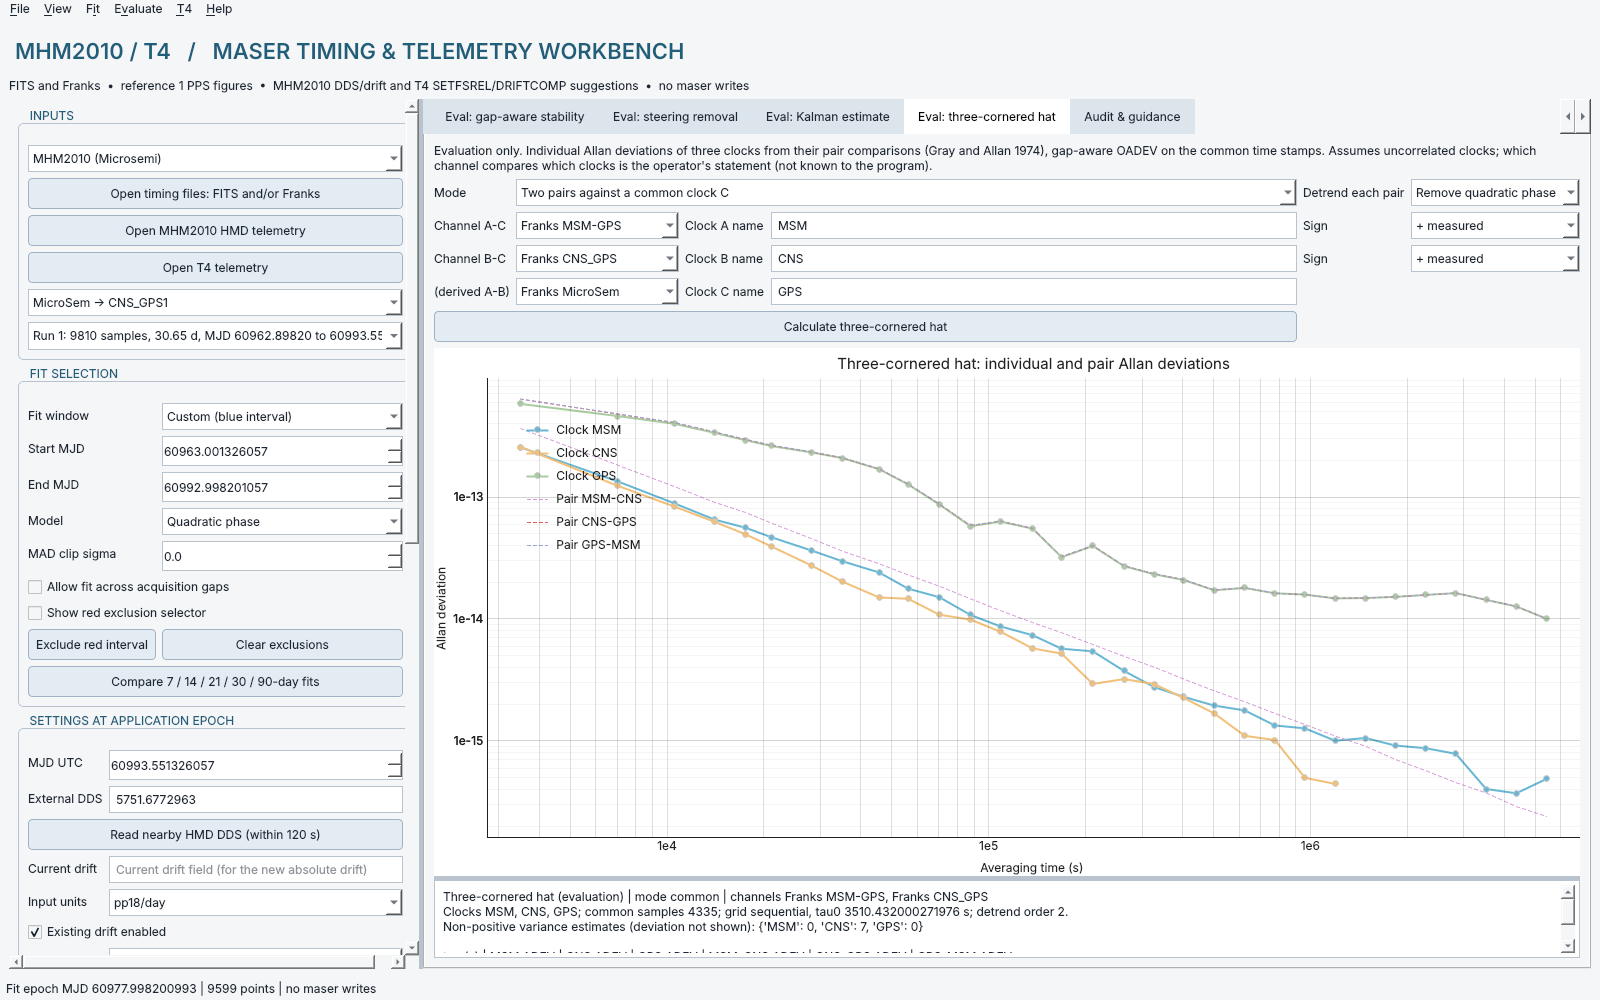
\includegraphics[width=.92\linewidth]{../validation/gui_0.3.0/gui_eval_three_cornered_hat_light.png}
\end{cfigure}
\begin{cfigure}{Veusz 3.6.2 renders of the evaluation pages: \texttt{GapStab\_fractional\_frequency}, \texttt{Steer\_\ldots\_phase\_mjd}, \texttt{Kalman\_\ldots\_frequency\_mjd} and \texttt{TCH\_allan\_deviation}.\label{fig:veuszeval}}
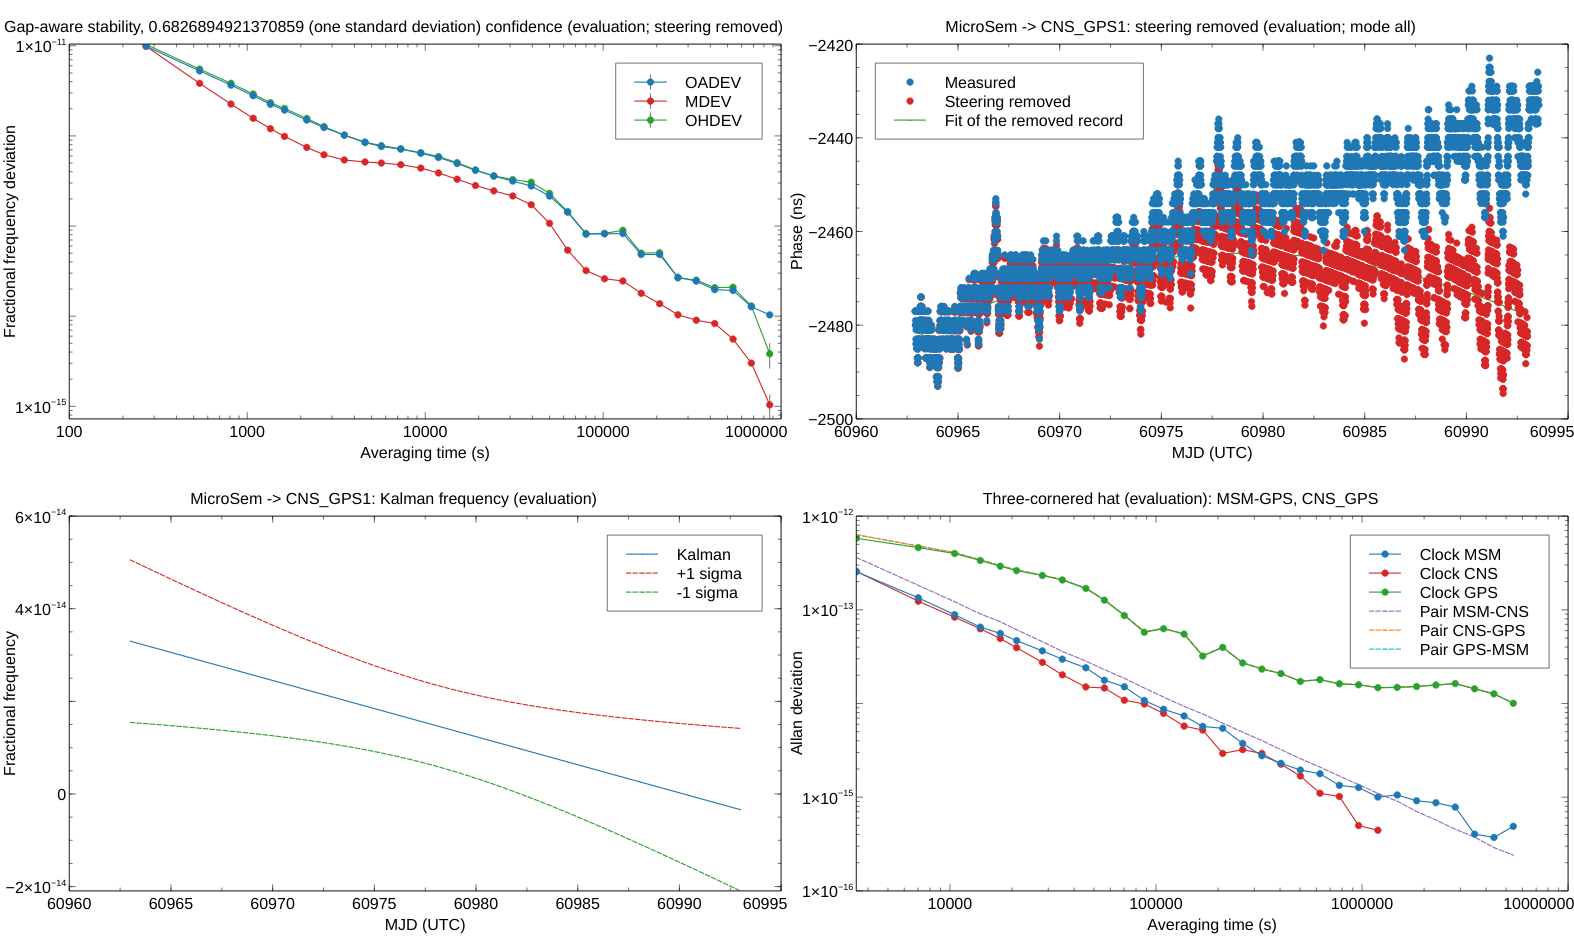
\includegraphics[width=\linewidth]{../validation/veusz_render_v0.3.0/evaluation_contact_sheet.png}
\end{cfigure}
\warning{The evaluation tabs inform the review; they do not certify a setting. The steering removal
depends on the HMD column that drives the output, the Kalman uncertainties on a noise model that fits
only approximately, and the three-cornered hat on the operator's statement of which channel compares
which clocks and on their independence.}
\clearpage
\section{Output package and reproducibility}\label{sec:output}
\subsection{Files of an analysis export}
\begin{ctable}{Files of an analysis export folder\label{tab:outputs}}
\begin{tabular}{@{}P{.36\linewidth}P{.59\linewidth}@{}}
\toprule
Output & Meaning\\
\midrule
\texttt{analysis.vszh5} & Native HDF5 document, typed datasets and Veusz plotting script; pages as ticked\\
\texttt{analysis.json} & Fit, coefficients, conditional covariance, settings, both drift units, provenance, warnings;
0.3.0: \texttt{export\_content}, \texttt{evaluation}, \texttt{evaluation\_files} (strict JSON: NaN written as \texttt{null})\\
\texttt{phase\_and\_fit.csv} & All input timing samples, model, residual, selection and fit masks\\
\texttt{telemetry\_overlap.csv} & HMD rows overlapping the selected timing interval, if present\\
\texttt{stability.csv} & Base estimator, tau, deviation and overlapping-term count\\
\texttt{raw.PHD / raw.FRD} & Optional uniform-record Stable32 phase and fractional frequency\\
\texttt{fit\_residual.*} & Separately identified residual stability inputs\\
\texttt{evaluation\_gap\_stability.csv} & 0.3.0, when ticked: gap-aware estimators with intervals (Table~\ref{tab:evalcolumns})\\
\texttt{evaluation\_steering\_removed.csv} & 0.3.0, when ticked: measured, applied and steering-removed phase\\
\texttt{evaluation\_kalman.csv} & 0.3.0, when ticked: Kalman phase, frequency, drift, innovations\\
\texttt{evaluation\_three\_cornered\_hat.csv} & 0.3.0, when ticked: clock and pair Allan deviations\\
\texttt{review.md} & Human-readable advisory summary, reference table; 0.3.0 adds ``Veusz content'' and ``Further evaluation''\\
\bottomrule
\end{tabular}
\end{ctable}

The HDF5 document is written using the supplied writer without importing
Veusz. All measured raw pair datasets and descriptive labels are included when
the full collection is exported. Overview medians are separate datasets.
The example's externally rendered PDF is a preview, not a dependency of the
application.

Exports first build in a temporary adjacent folder and rename only after
success. An existing destination is rejected. This protects earlier results
on ordinary local filesystems; no distributed-filesystem transactional
guarantee is claimed. The CSV, JSON and text files are always complete: unticking a page group
removes pages and their datasets from the \texttt{.vszh5} only.

\begin{ctable}{Columns of the evaluation CSV files (every number exact)\label{tab:evalcolumns}}
\begin{tabular}{@{}P{.3\linewidth}P{.65\linewidth}@{}}
\toprule
File & Columns\\
\midrule
\texttt{evaluation\_gap\_stability.csv} & \texttt{estimator}, \texttt{tau\_s}, \texttt{deviation}, \texttt{ci\_low},
\texttt{ci\_high}, \texttt{ci\_method}, \texttt{terms}, \texttt{edf}, \texttt{noise\_alpha}, \texttt{noise\_type},
\texttt{differences\_d}\\
\texttt{evaluation\_steering\_removed.csv} & \texttt{mjd\_utc}, \texttt{measured\_phase\_s},
\texttt{applied\_fractional\_frequency}, \texttt{applied\_phase\_s}, \texttt{steering\_removed\_phase\_s},
\texttt{covered\_by\_hmd}\\
\texttt{evaluation\_kalman.csv} & \texttt{mjd\_utc}, \texttt{measured\_phase\_ns}, \texttt{phase\_ns},
\texttt{phase\_sigma\_ns}, \texttt{fractional\_frequency}, \texttt{fractional\_frequency\_sigma},
\texttt{drift\_per\_day}, \texttt{drift\_sigma\_per\_day}, \texttt{innovation\_ns}, \texttt{innovation\_sigma\_ns}\\
\texttt{evaluation\_three\_cornered\_hat.csv} & \texttt{tau\_s}; per clock \texttt{clock\_<name>\_variance},
\texttt{clock\_<name>\_adev}; per pair \texttt{pair\_<A-B>\_adev}, \texttt{pair\_<A-B>\_terms}\\
\bottomrule
\end{tabular}
\end{ctable}

\subsection{Veusz pages to generate}\label{sec:pages}
OUTPUT $\rightarrow$ \textbf{Veusz pages to generate} decides which page groups
\texttt{analysis.vszh5} receives. Base groups are on by default (the file is then the 0.2.4 file);
evaluation groups are off. \textbf{Defaults} restores that; \textbf{All} ticks everything. A page is
written only when its data exist (for example, no HMD pages without HMD). A ticked evaluation group is
recalculated from the current fit at export time with the options of its tab; if it cannot be
calculated (for example steering removal without HMD) it is left out with a note in the audit tab, and
the base export continues.

\begin{ctable}{Veusz page groups: checkbox, default, batch flag and pages\label{tab:pagegroups}}
\footnotesize
\begin{tabular}{@{}P{.26\linewidth}P{.07\linewidth}P{.2\linewidth}P{.39\linewidth}@{}}
\toprule
Checkbox (\texttt{ExportContent} name) & Default & Batch flag & Pages (\texttt{<ch>} is the channel name)\\
\midrule
1 PPS reference figures (with the suggested-changes box) (\texttt{reference\_figures}) & on & \texttt{--no-reference-figures} &
\texttt{Ref1PPS\_<ch>\_deltas\_MJD}, \texttt{\_fit\_MJD}, \texttt{\_deltas\_local}, \texttt{\_fit\_local}\\
Selected channel: phase, fit and residual pages (\texttt{timing\_pages}) & on & \texttt{--no-timing-pages} &
\texttt{Selected\_<ch>\_phase\_and\_fit\_mjd/\_local}, \texttt{Fit\_<ch>\_residual\_mjd/\_local}\\
Timing overview of every channel (\texttt{overview}) & on & \texttt{--no-overview} & \texttt{Overview\_<channel>\_mjd/\_local}\\
Stability (base tab, when calculated) (\texttt{stability}) & on & \texttt{--no-stability-pages} &
\texttt{Stability\_fractional\_frequency}, \texttt{Stability\_TDEV}\\
HMD telemetry plots (MHM2010) (\texttt{hmd\_telemetry}) & on & \texttt{--no-hmd-plots} &
\texttt{HMD\_DDS\_change\_counts\_mjd/\_local}, \texttt{HMD\_DDS\_setting\_mjd/\_local}, \texttt{HMD\_all\_channels\_MJD\_1\ldots}\\
T4 MONIT telemetry plots (\texttt{t4\_telemetry}) & on & \texttt{--no-t4-plots} & \texttt{T4\_MONIT\_<group>\_*}, \texttt{T4\_MONIT\_main\_PLL\_lock\_*}\\
T4 monitoring-file plots (\texttt{t4\_monitoring\_files}) & on & \texttt{--no-t4-monitoring-plots} & \texttt{T4log\_<layout>\_<unit>\_*}, \texttt{\_status\_*}\\
Evaluation: gap-aware stability with confidence intervals (\texttt{gap\_stability}) & off & \texttt{--gap-stability} &
\texttt{GapStab\_fractional\_frequency}, \texttt{GapStab\_TDEV}\\
Evaluation: steering events removed (needs HMD) (\texttt{steering\_removed}) & off & \texttt{--remove-steering} &
\texttt{Steer\_<ch>\_phase\_mjd/\_local}, \texttt{Steer\_HMD\_<column>\_applied\_mjd/\_local}\\
Evaluation: Kalman estimate (\texttt{kalman}) & off & \texttt{--kalman} &
\texttt{Kalman\_<ch>\_frequency}, \texttt{\_drift}, \texttt{\_innovation} (each \texttt{\_mjd/\_local})\\
Evaluation: three-cornered hat (\texttt{three\_cornered\_hat}) & off & \texttt{--tch CH \ldots} & \texttt{TCH\_allan\_deviation}\\
\bottomrule
\end{tabular}
\end{ctable}
\begin{cfigure}{OUTPUT box with the ``Veusz pages to generate'' checkboxes (Light theme).\label{fig:guicheck}}
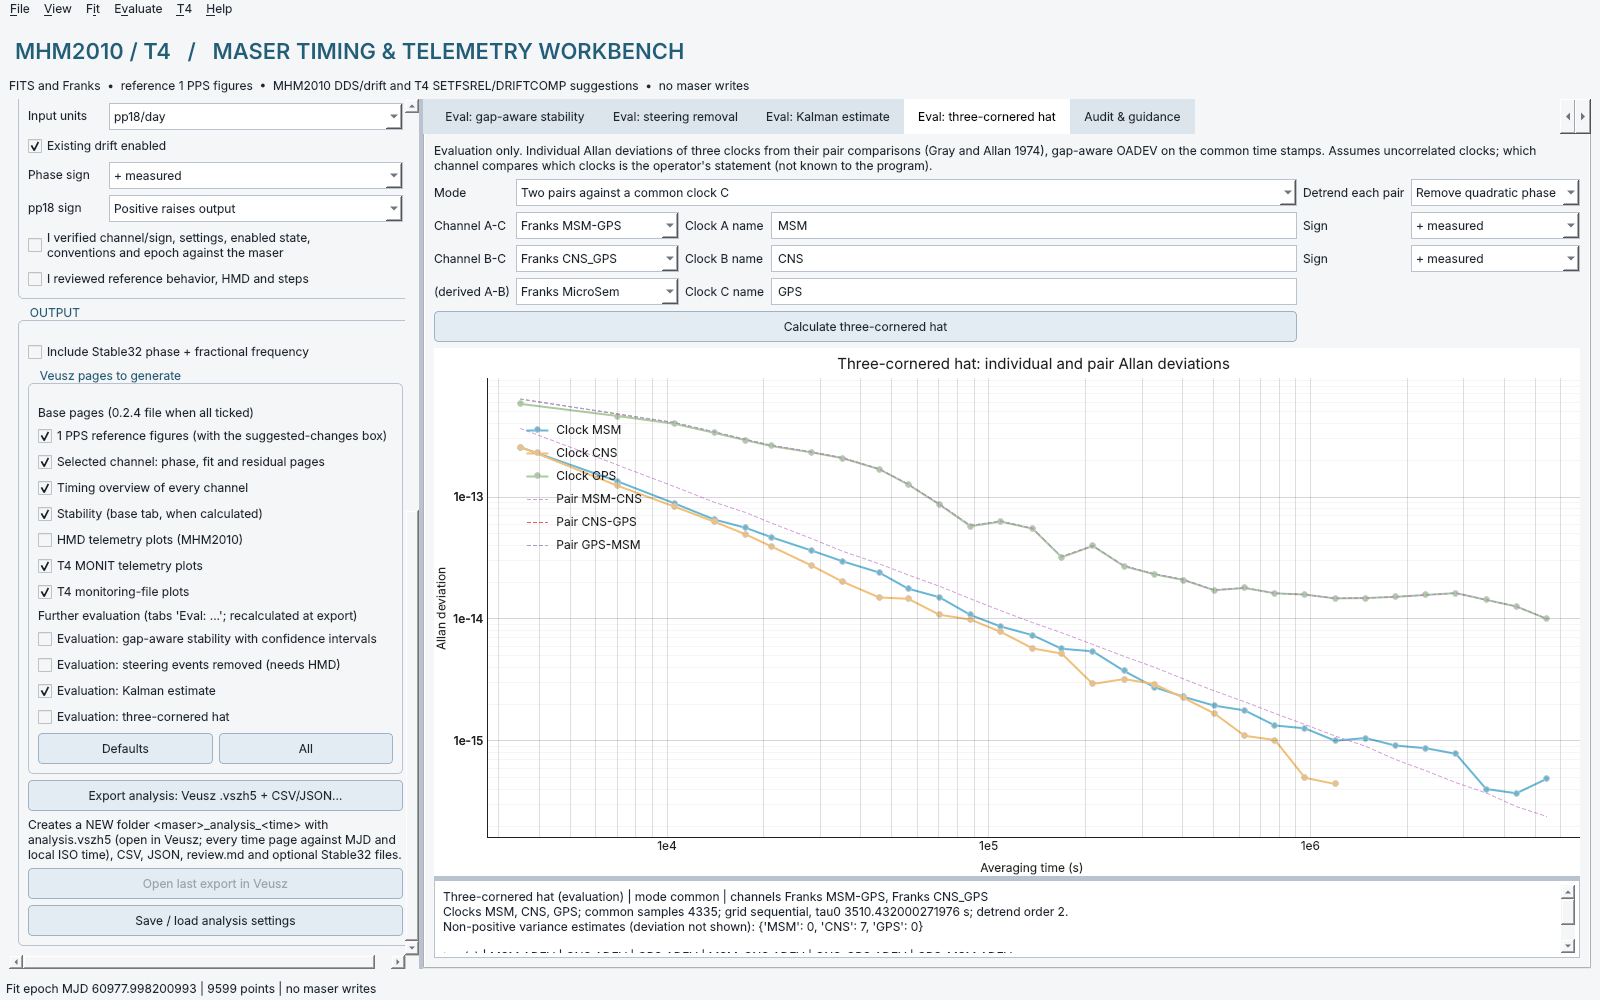
\includegraphics[width=.6\linewidth]{../validation/gui_0.3.0/gui_output_checkboxes_light.png}
\end{cfigure}
The default document of 0.3.0 was compared with 0.2.4 by a fingerprint of every dataset (SHA-256 of the
values), every tag, every page and the plotting script (with the creation time removed): identical
(\texttt{tools/export\_fingerprint.py}, \texttt{tests/data/export\_fingerprint\_0.2.4.json}).

\subsection{Where the Veusz files are}
The \texttt{.vszh5} files are written only by an export, always into a \emph{new} folder:
\begin{ctable}{Where each action writes its Veusz file\label{tab:wherevszh5}}
\begin{tabular}{@{}P{.36\linewidth}P{.58\linewidth}@{}}
\toprule
Action & Result\\
\midrule
File $\rightarrow$ Export analysis folder (Ctrl+E), or OUTPUT $\rightarrow$ ``Export analysis: Veusz
.vszh5 + CSV/JSON'' & \texttt{<parent>/<MHM2010|T4>\_analysis\_}\allowbreak\texttt{<YYYYMMDDTHHMMSS$\pm$hhmm>/}\allowbreak\texttt{analysis.vszh5}
(needs a valid fit)\\
File $\rightarrow$ Export T4 data (Ctrl+Shift+E), or the T4 tabs' export buttons &
\texttt{<parent>/T4\_telemetry\_export\_<time>/}\allowbreak\texttt{t4\_telemetry.vszh5}\\
\texttt{analyze\_maser.py \dots --output DIR} & \texttt{DIR/analysis.vszh5} (path printed as
\texttt{veusz\_file})\\
\texttt{t4\_native.py FILES --output DIR} & \texttt{DIR/t4\_telemetry.vszh5}\\
\bottomrule
\end{tabular}
\end{ctable}
After a GUI export a dialog shows the full path with \textbf{Open in Veusz} and \textbf{Open folder};
``Open last export in Veusz'' (OUTPUT box and File menu) reopens it. Veusz is looked for at the path set
with File $\rightarrow$ Set Veusz program, then on PATH, then in
\texttt{Program Files\textbackslash Veusz}; if not found, the program asks once. Veusz 3.6 or later opens
\texttt{.vszh5} directly.
\begin{cfigure}{Export dialog with Open in Veusz and Open folder.\label{fig:exportdialog}}
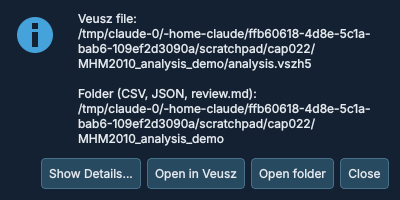
\includegraphics[width=.45\linewidth]{../validation/gui_export_dialog.png}
\end{cfigure}

\subsection{Exports: names, tags and full precision}\label{sec:exports}
\textbf{No rounding.} Numeric datasets are float64. Numbers written as text use the shortest decimal that
reads back to the same binary64 value (Python \texttt{repr}, at most 17 significant digits [15]); CSV
files are written by pandas without a float format and read back bit-identical (tested). Earlier
releases wrote the T4 CSVs with \texttt{\%.6g} (5751.6770000 became 5751.68) and shortened file hashes
in the notes; both are fixed. Figure boxes keep the figure layout; every number in them is also a
one-element dataset and a line in \texttt{\_results\_full\_precision\_text}. Release 0.2.4 extends
this to times written as text and to the T4 live recorder (section ``\nameref{sec:exacttime}'');
release 0.3.0 writes the evaluation results the same way (the confidence level in a page title is the
full value, \texttt{0.6826894921370859 (one standard deviation)}).

Veusz's Data-editor table displays any float with 6 significant digits (Qt's default display; Veusz
3.6.2 \texttt{dialogs/dataeditdialog.py}) although the file holds every digit: double-click a cell,
or open a \texttt{*\_text} dataset. Axes use the tick format \texttt{\%.12Vg} (up to 12 digits;
Veusz's automatic \texttt{\%Vg} shows MJD 60975 as \(6.0975\times10^4\)).

\begin{ctable}{Dataset names (examples)\label{tab:names}}
\begin{tabular}{@{}P{.5\linewidth}P{.44\linewidth}@{}}
\toprule
Dataset (examples) & Meaning\\
\midrule
\texttt{Franks\_MSM\_GPS\_phase\_ns}, \texttt{FITS\_Site1Hz\_to\_CNS\_GPS1\_phase\_ns} & every input channel\\
\texttt{Selected\_MSM\_GPS\_time\_MJD\_UTC}, \texttt{\_time\_local}, \texttt{\_phase\_ns} & the analysed channel\\
\texttt{Fit\_MSM\_GPS\_model\_phase\_ns}, \texttt{\_residual\_ns}, \texttt{\_used\_in\_fit\_flag} & the selected model\\
\texttt{Ref1PPS\_MSM\_GPS\_deltas\_ns}, \texttt{\_fit\_line\_ns}, \texttt{\_fit\_a1\_ns\_per\_day} & reference figures and their numbers\\
\texttt{Suggested\_MHM2010\_dds\_change\_counts}, \texttt{\_drift\_change\_pp18\_per\_day} & suggested changes\\
\texttt{HMD\_ExtSynth\_32}, \texttt{HMD\_ExtSynth\_32\_\allowbreak change\_counts}, \texttt{\_text} & HMD telemetry\\
\texttt{T4log\_MonitHCB\_\allowbreak Internal\_temperature\_degC} & T4 monitoring file\\
\texttt{T4\_MONIT\_ch05\_<short>\_V}, \texttt{\_code} & T4 MONIT telemetry\\
\texttt{Stability\_OADEV\_tau\_s}, \texttt{\_deviation}, \texttt{\_terms} & base stability\\
\texttt{GapStab\_OADEV\_deviation} (with \(\pm\) errors), \texttt{\_ci\_low}, \texttt{\_ci\_high}, \texttt{\_edf}, \texttt{\_noise\_alpha} & gap-aware stability (0.3.0)\\
\texttt{Steer\_<ch>\_steering\_removed\_phase\_ns}, \texttt{\_applied\_phase\_ns}, \texttt{Steer\_HMD\_ExtSynth\_32\_DDS\_used} & steering removal (0.3.0)\\
\texttt{Kalman\_<ch>\_fractional\_frequency}, \texttt{\_sigma}, \texttt{\_plus\_1sigma}, \texttt{\_innovation\_ns} & Kalman estimate (0.3.0)\\
\texttt{TCH\_tau\_s}, \texttt{TCH\_clock\_<name>\_adev}, \texttt{TCH\_pair\_<A\_B>\_adev} & three-cornered hat (0.3.0)\\
\bottomrule
\end{tabular}
\end{ctable}
Names use letters, digits and \texttt{\_} only, so each is also a Veusz expression (a pair name such as
\texttt{MSM-CNS} becomes \texttt{MSM\_CNS}). With writer 0.0.27 and later the traces take the y dataset
name and graphs \texttt{g\_<y>}, so the widget tree reads like the data. Appendix C lists every stability
dataset.

\textbf{Tags.} Every dataset carries one \texttt{source\_*} tag (\texttt{Franks}, \texttt{FITS}, \texttt{HMD},
\texttt{T4\_MONIT\_UDP}, \texttt{T4\_log\_<layout>}, \texttt{Workbench}) and one or more
\texttt{type\_*} tags (\texttt{time\_MJD}, \texttt{time\_local}, \texttt{time\_text},
\texttt{measurement}, \texttt{fit\_model}, \texttt{fit\_residual}, \texttt{fit\_results},
\texttt{suggested\_settings}, \texttt{telemetry}, \texttt{status}, \texttt{stability},
\texttt{reference\_figure}, \ldots; 0.3.0 adds \texttt{evaluation}, \texttt{steering}, \texttt{kalman} and
\texttt{metadata}). In Veusz choose Data $\rightarrow$ \emph{Group by: Tags}; a dataset appears under each of its
tags [14]; \texttt{type\_evaluation} gathers every evaluation dataset.

\textbf{HMD telemetry.} The analysis export holds every HMD column over the fit interval, the DDS columns
(\texttt{ExtSynth\_32}, \texttt{Thumbwheels\_31}) also as a change in counts from the first value and as
exact text, pages for the DDS change and setting, and overview pages of ten panels. In the historical
example (Oct.--Nov.\ 2025) \texttt{ExtSynth\_32} falls by about 13 counts/day while
\texttt{Thumbwheels\_31} stays at 5751.6774093; release 0.3.0 confirms that this is the drift
compensation acting on the DDS: removing it changes the fitted drift by exactly the recorded ramp
(section ``\nameref{sec:evalresults}'').
\begin{cfigure}{HMD DDS change in counts against MJD (Veusz 3.6.2 render, historical month).\label{fig:hmddds}}
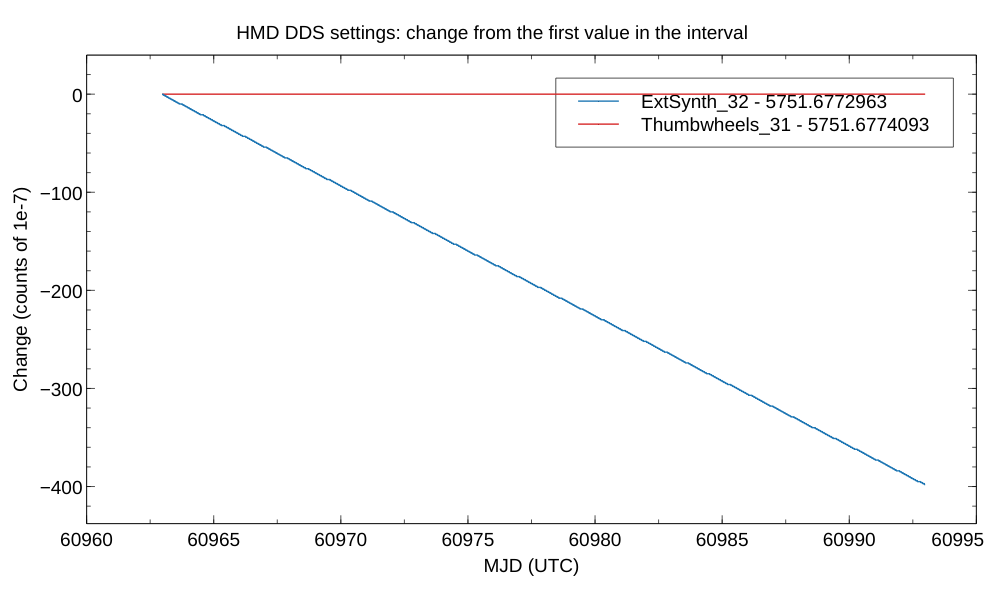
\includegraphics[width=.8\linewidth]{../validation/veusz_render_v0.2.3/hmd_analysis_p08_HMD_DDS_change_counts_mjd.png}
\end{cfigure}

\subsection{Exact times as text}\label{sec:exacttime}
Releases up to 0.2.3 wrote local times with \texttt{datetime.isoformat(timespec="seconds")}, which
\emph{cuts} the fraction: the application epoch of the 2026 Franks example, MJD 61234.10355, read
\texttt{2026-07-12T22:29:06-04:00} although it is 22:29:06.72. Microseconds are not enough either:
the spacing of binary64 numbers [15] near the values used here is finer than Python's 1~\(\mu\)s
\texttt{datetime}:
\begin{ctable}{Spacing of binary64 numbers near the time values used\label{tab:binary64}}
\begin{tabular}{@{}lll@{}}
\toprule
Quantity & Value near & binary64 spacing\\
\midrule
MJD (days) & 61220 & \(7.28\times10^{-12}\) d \(=0.63\ \mu\)s\\
Unix time (s) & \(1.79\times10^{9}\) & \(0.24\ \mu\)s\\
\bottomrule
\end{tabular}
\end{ctable}
Writer 0.0.29 takes the shortest decimal that reads back as the same binary64 MJD (Python
\texttt{repr}) and converts it in decimal arithmetic [16] with 80 significant digits, so no step rounds.
\begin{vartable}{tab:var-T}{Variables of the exact time text (T1--T2)}
\(M\) & shortest decimal that reads back as the binary64 MJD (Python \texttt{repr}) & day\\
\(t\) & Unix seconds of \(M\), in decimal arithmetic & s\\
\(o(t)\) & zone offset at instant \(t\) (daylight saving included) & s\\
\(w\) & local wall-clock seconds, \(t+o(t)\) & s\\
\(\lfloor w\rfloor\) & whole seconds of \(w\) & s\\
\(\operatorname{ISO}(\cdot)\), \(\operatorname{digits}(\cdot)\) & ISO 8601 date-time of whole seconds; all decimal digits of the fraction, no trailing zeros & --\\
text & the written time, e.g.\ \texttt{2026-07-12T22:29:06.72-04:00} & --\\
\end{vartable}
\begin{gather}
t=(M-40587)\times86400\ \mathrm{s},\qquad
w=t+o(t),\qquad
\text{text}=\operatorname{ISO}\bigl(\lfloor w\rfloor\bigr)\,.\,\text{digits}\bigl(w-\lfloor w\rfloor\bigr)\ \pm\mathrm{HH{:}MM}, \tag{T1}\label{eq:T1}\\
M=\frac{t}{86400}+40587,\qquad t=w-o. \tag{T2}\label{eq:T2}
\end{gather}
The inverse (T2), evaluated in decimal arithmetic, gives back the identical binary64 MJD (tested for
10\,000 random values in five zones and for every Franks sample) [12]. A Franks MJD has 5 decimals
(\(10^{-5}\) d \(=0.864\) s), so its text has at most 3 decimals of a second.

\begin{ctable}{Time text in 0.2.3 and from 0.2.4 on\label{tab:timetext}}
\begin{tabular}{@{}P{.3\linewidth}P{.3\linewidth}P{.32\linewidth}@{}}
\toprule
Where & 0.2.3 & 0.2.4 and later\\
\midrule
\texttt{Selected\_MSM\_GPS\_\allowbreak time\_local\_\allowbreak ISO\_text} & \texttt{2025-12-31T19:30:06-05:00} & \texttt{2025-12-31T19:30:06.624-05:00}\\
Suggested-changes box & \texttt{22:29:06-04:00 (MJD 61234.10355)} & \texttt{22:29:06.72-04:00 (MJD 61234.10355)}\\
\(\mathrm{MJD}-\mathrm{MJD}_0\) label, FITS \(M_0\) & \texttt{MJD - 61349.71235} & \texttt{MJD - 61349.7123456789}\\
T4 log text & from the MJD (whole s cut) & the T4's whole seconds, \texttt{12:13:09-05:00}\\
T4 recorder CSV & \texttt{\%.10f} MJD (8.64 \(\mu\)s), \texttt{\%.3f}, \texttt{\%.6g} & every digit (\texttt{repr})\\
\bottomrule
\end{tabular}
\end{ctable}
The writer also offers \texttt{iso\_local\_strings(epoch, timespec="exact")} for times that start as
Unix seconds (e.g.\ a host clock); its default (\texttt{"seconds"}) is unchanged for every other
program. The statistics/fit box keeps the layout of the reference figures; every number in it is a
full-precision dataset. A new DDS value is quantized to the 7 decimals the MHM2010 accepts, with the
exact change and the residual reported beside it.

\subsection{MJD and local ISO 8601 time axes}
Veusz stores dates as naive seconds from 2009-01-01, so a local wall-clock axis needs the zone offset
of each sample.
\begin{vartable}{tab:var-V}{Variables of the Veusz local time axis (V1)}
\(V_i\) & Veusz date value of sample \(i\): naive local seconds since 2009-01-01T00:00:00 & s\\
\(t_i^{\mathrm{Unix}}\) & Unix seconds of sample \(i\) & s\\
\(\mathrm{MJD}_i\) & Modified Julian Date of sample \(i\), UTC & day\\
\(o(t_i)\) & UTC offset of the processing computer at sample \(i\) (daylight saving aware) & s\\
1\,230\,768\,000 & Unix seconds of 2009-01-01T00:00:00 UTC & s\\
\end{vartable}
\begin{equation}
V_i=t_i^{\mathrm{Unix}}-1\,230\,768\,000\ \mathrm{s}+o(t_i),\qquad
t_i^{\mathrm{Unix}}=(\mathrm{MJD}_i-40587)\times86400\ \mathrm{s}. \tag{V1}\label{eq:V1}
\end{equation}
The tick format is \verb|%VDY-%VDm-%VDdT%VDH:%VDM:%VDS| followed by
the offset, e.g.\ \texttt{2026-11-03T06:31:15-05:00}. Veusz formats are static, so when the data
cross a DST change the ticks omit the offset and the axis label lists each offset and when it
begins. Each time-series page is written twice (\texttt{\dots\_mjd}, \texttt{\dots\_local}); the
reference figures keep the operator's $\mathrm{MJD}-\mathrm{MJD}_0$ axis and gain
\texttt{\_deltas\_local} and \texttt{\_fit\_local}. Writer helpers: \texttt{mjd\_to\_epoch},
\texttt{local\_time\_axis}, \texttt{iso\_local\_strings}, \texttt{time\_pair\_pages}.
\begin{cfigure}{Veusz 3.6.2 renders from \texttt{analysis.vszh5}: fit page against \(\mathrm{MJD}-\mathrm{MJD}_0\), and the deltas twin against local ISO time (EDT in June).\label{fig:axes}}
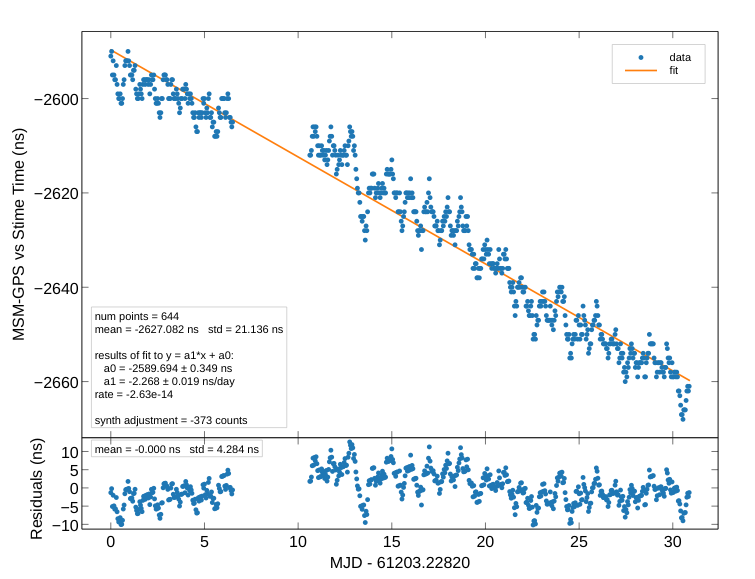
\includegraphics[width=.8\linewidth]{../validation/veusz_render_v0.2.0/analysis_p01_pps_fit.png}\\[4pt]
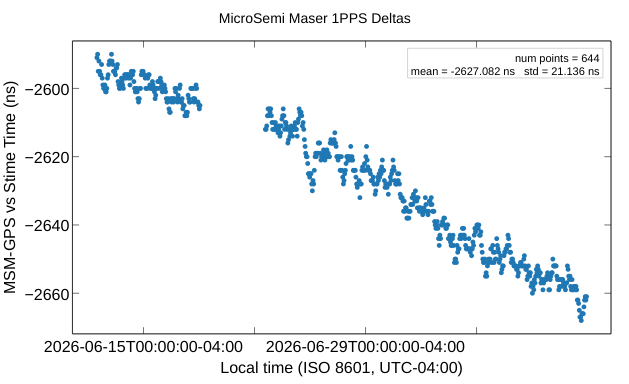
\includegraphics[width=.62\linewidth]{../validation/veusz_render_v0.2.0/analysis_p02_pps_deltas_local.png}
\end{cfigure}

\subsection{Batch operation}
\begin{lstlisting}
python analyze_maser.py --fits-directory <FITS_DIRECTORY>
  --hmd <HMD_FILE> --start 2025-10-15 --end 2025-11-14
  --derive-dds --drift 975 --sampling-tolerance .02
  --stable32 --output <NEW_OUTPUT_DIRECTORY>
\end{lstlisting}
Join the lines for the shell. The end time is exclusive. Without DDS and drift
inputs, the batch path exports measurement results without a correction
candidate. \texttt{--derive-dds} only copies an HMD setting within 120 s of the
historical application epoch; it does not retrieve present-day state.

With the 0.3.0 flags, the following adds every evaluation and leaves the HMD plots out of the
\texttt{.vszh5} (the HMD CSV and JSON stay complete):
\begin{lstlisting}
python analyze_maser.py --fits-directory <FITS_DIRECTORY> --hmd <HMD_FILE>
  --start 2025-10-15 --end 2025-11-14 --derive-dds --output <NEW_OUTPUT_DIRECTORY>
  --gap-stability --gap-source steering-removed --gap-detrend 2
  --remove-steering --kalman --no-hmd-plots
python analyze_maser.py --timing-directory <FRANKS_DIRECTORY> --channel MSM-GPS
  --output <NEW_OUTPUT_DIRECTORY> --tch MSM-GPS CNS_GPS --tch-mode common
  --tch-names MSM CNS GPS
\end{lstlisting}
\texttt{--remove-steering} (or \texttt{--gap-source steering-removed}) without \texttt{--hmd} stops with
an error. The printed JSON lists \texttt{evaluation\_files}. Batch evaluation never changes the printed
\texttt{suggested\_settings}: for the 2026 Franks MSM-GPS channel, last 30 days, the JSON is identical with
and without \texttt{--gap-stability --kalman --tch}, with a DDS change of \(-526.7884344769938\) counts
in both.

\subsection{Writer revision}
The attached writer was version 0.0.21. A targeted test demonstrated that
\texttt{dataset\_date()} accepted multidimensional input, creating invalid
date shape or silently flattening it in resizable mode. Version 0.0.22 adds
one-dimensional validation before creating the dataset group. Valid callers
retain the same API. This is a scoped defect correction, not an exhaustive
review of every writer feature.

Release 0.2.0 shipped 0.0.24 (MJD and local ISO time axes). Release 0.2.3 ships 0.0.27, copied
unchanged from the operator's FitsAutoPlot folder (SHA-256 \texttt{992e46a4\ldots40be2369}); it names
graphs and traces after their data. The registry master 0.0.28 differs only in saving speed and writes
identical files; see \texttt{docs/vszh5\_writer\_0.0.27\_NOTES.md}.

Release 0.2.4 ships 0.0.29: the registry master 0.0.28 (FitsAutoPlot 0.4.1, faster saving, identical
files), rebuilt from 0.0.27 and matched to the master byte for byte (SHA-256
\texttt{13f68513\ldots f634a64b5}), plus 0.0.29, made from the master for this release (additions
only: exact ISO 8601 text, section ``\nameref{sec:exacttime}''). Every 0.0.28 call writes the same file;
see \texttt{docs/vszh5\_writer\_0.0.29\_NOTES.md} and \texttt{docs/writer\_0.0.29/}. Release 0.3.0 ships the
same 0.0.29 unchanged (SHA-256 \texttt{50631331\ldots 4f9d701}); the evaluation pages use its existing
helpers (\texttt{xy\_page}, \texttt{time\_pair\_pages}, \texttt{dataset\_1d} with error bars).
\clearpage

\section{Historical validation results}\label{sec:historical}
The uploaded archive contains 109 FITS.GZ files and 40 measured channel pairs,
9,810 records per pair. The example selects October 15 through November 13,
2025, producing 9,600 direct MicroSem-to-CNS\_GPS1 samples. The HMD record covers
April 9, 2025, through March 25, 2026. The previously supplied July 2026 timing
files do not overlap that HMD record.

At the last selected sample, November 13, 2025, 23:57:24.571 UTC, the quadratic
fit gives frequency error \(+5.83844\times10^{-15}\), residual drift
\(-660.833\) parts in \(10^{18}\)/day and phase-residual RMS 5.405 ns.
These are computed results from the supplied files, not external instrument
specifications.

\warning{The example assumes enabled drift \(+975\) pp18/day and a positive
pp18 sign that raises output frequency. The older screenshot supplies that
example number, but does not establish its value in November (the HMD ramp of that month corresponds
to about 933 pp18/day, section ``\nameref{sec:evalresults}''). The following candidates are historical
and unapproved.}

\begin{ctable}{Historical example: candidate settings (not for entry)\label{tab:historical}}
\begin{tabular}{@{}P{.49\linewidth}r@{}}
\toprule
Quantity & Historical example\\
\midrule
HMD DDS near the last timing sample & 5751.6772565\\
Calculated DDS increment, last digits & +82.929597\\
New rounded DDS & 5751.6772648\\
New drift, pp18/day & +1635.833066\\
Equivalent new drift, DDS units/day & -23.235467\\
Nearest integer pp18/day alternative & +1636\\
Nearest integer DDS units/day alternative & -23\\
\bottomrule
\end{tabular}
\end{ctable}

\subsection{The dominant warning: fit-window sensitivity}
\begin{ctable}{Historical example: trailing-window sensitivity\label{tab:window}}
\begin{tabular}{@{}rrrr@{}}
\toprule
Window, d & Frequency error at common end & Drift, pp18/day & RMS, ns\\
\midrule
30 & \(+5.83844\times10^{-15}\) & -660.833 & 5.405\\
21 & \(+3.80025\times10^{-15}\) & -883.575 & 5.810\\
14 & \(+1.39421\times10^{-14}\) & +407.199 & 5.922\\
7  & \(-4.32655\times10^{-15}\) & -5454.180 & 6.970\\
\bottomrule
\end{tabular}
\end{ctable}
The drift changes sign with the fitting interval. Conditional OLS errors are
much smaller than this variation and must not be interpreted as a complete
uncertainty budget. The Kalman estimate of 0.3.0 gives a drift uncertainty of about
\(\pm1.0\times10^{-15}\)/day (1013 pp18/day) for the 30-day window, consistent with this spread.
A longer/reference-checked operating-state review is needed before any live adjustment.

For the 30-day window, CNS2018 and CNS\_GPS2 comparisons give \(-688.966\)
and \(-652.571\) pp18/day. Similar values are useful but do not demonstrate
independent references or isolate maser aging.
\clearpage

\section{Cross-checks, testing and limitations}
\subsection{Franks/Veusz comparison}
The supplied Veusz example was read as HDF5 data, without executing its
embedded plotting script. Across 735 matching UTC-hour bins in the full
archive span, the new derived MSM--GPS comparison differs by 1.284 ns RMS
from the historical reduced values. MicroSem and CNS\_GPS1 differ by
0.852 ns and 1.004 ns RMS. Median differences are approximately zero.
The maximum absolute differences are 4, 2 and 4 ns respectively.

These small differences are consistent with nonidentical reduction windows
and rounding, but that explanation is not a proof of identical processing.
The direct raw pair remains the primary correction input. Invalid negative
MJD legacy records and all-missing channels in the exemplar were not copied.

\subsection{Automated and rendering checks}
The 0.1.0 suite had 36 tests; release 0.3.0 has 174 (Python 3.13.18, offscreen Qt). Tests cover analytic
phase coefficients, DDS direction, quantization, both drift representations,
disabled drift, reversal, duplicates, gap/grid rejection, clipping, FITS
metadata/padding, Franks sentinels, GUI controls/settings, writer behavior,
export protection, exact exports, names and tags, time text, the T4 and, from 0.3.0, the evaluation methods,
page selection and the unchanged suggestion.

OADEV, MDEV, TDEV and OHDEV were compared with AllanTools \allantools\ for seeded synthetic
phase data, including contributing-term counts; the gap-aware estimators, noise identification, EDF and
intervals were compared with AllanTools too. The 33-page 0.3.0 \texttt{analysis.vszh5} with every group ticked
was rendered with Veusz 3.6.2 (\texttt{validation/veusz\_render\_v0.3.0/}). GUI captures document the offscreen
Qt tests (\texttt{validation/gui\_0.3.0/}).

\subsection{Not validated}
\begin{itemize}
\item \textbf{Windows/bracca}: actual desktop operation was not performed (packages are staged when the computer is online).
\item \textbf{Stable32 executable}: output structure was checked, but proprietary-application import remains a site test.
\item \textbf{Installed masermon}: sign, range, precision, update cadence, persistence and firmware/version behavior remain site checks.
\item \textbf{Physical system}: no live adjustment, calibration or post-adjustment monitoring was conducted.
\item \textbf{Uncertainty}: the 0.3.0 intervals and Kalman uncertainties rest on the identified noise and
approximate EDFs; no reference-error removal is claimed beyond the three-cornered hat, whose channel
definitions are the operator's statement.
\item \textbf{HMD selector codes}: which synthesizer drives the output is not decoded (steering removal assumes the external DDS).
\item \textbf{Veusz 4.2.1}: the new pages were rendered with 3.6.2 only.
\end{itemize}

\subsection{Repository provenance}
The RF\_Equipment\_Comms stability-tool code
\href{https://github.com/Braveheart53/RF_Equipment_Comms/tree/main/sa_stability_tool}{[5]}
and FitsAutoPlot sources \href{https://github.com/Braveheart53/FitsAutoPlot}{[6]}
were read for header, GUI and analysis conventions. The science modules in this package
are new implementations using the cited definitions, not a wholesale copy of
the signal-analyzer tool. Repository checkouts were read-only with respect
to their remotes; no push was performed.

Reviewed commits:
\begin{itemize}
\item RF\_Equipment\_Comms: \texttt{9305e94e9ad85dbdb94a3765cf0989449dc3f345}.
\item FitsAutoPlot: \texttt{36add38d973bc07e920ff70680a139241c421f7c}.
\end{itemize}
The product-page pointer is
\href{https://www.microchip.com/en-us/product/mhm-2010}{Microchip MHM-2010 [7]}.
\clearpage

\section{Validation by release}
\subsection{Release 0.3.0}
\begin{ctable}{Validation of release 0.3.0\label{tab:val030}}
\begin{tabular}{@{}P{.42\linewidth}P{.5\linewidth}@{}}
\toprule
Check & Result\\
\midrule
Test suite (Python 3.13.18, NumPy 2.5.4, pandas 3.1.0, SciPy 1.18.1, PySide6 6.12.0, h5py 3.16.0, AllanTools 2024.06; offscreen) & 174 passed in 47.08 s: 159 retained (one version check relaxed to ``0.2.4 or later''), 15 new\\
Default export vs 0.2.4 & identical fingerprint: every dataset's SHA-256, tags, pages and script\\
Base suggestion with every evaluation (GUI, batch) & identical suggestion JSON; Franks DDS change \(-526.7884344769938\) counts in both\\
Gap-free gap-aware estimators & equal to the base tab (\(10^{-12}\) relative) and AllanTools (\(10^{-9}\))\\
Gapped OADEV & equal to a brute-force sum over complete terms (\(10^{-12}\)); input values untouched\\
Noise type, EDF, chi-squared limits & noise type and differences identical to AllanTools; EDF and limits to \(10^{-12}\) relative\\
Sequential grid on jittered Franks data & every deviation inside its interval\\
Steering removal, synthetic & unsteered phase recovered to \(10^{-18}\) s; a 500-count step found in ``steps'' mode\\
Steering removal, historical month & drift difference equals the recorded ramp to 0.05\,\%\\
Kalman, simulated clock with a 200-sample gap & frequency within \(4\sigma\); NIS between 0.5 and 2; base unchanged\\
Three-cornered hat, three simulated clocks & each clock within 10\,\% (three-pair and common modes)\\
Page checkboxes & unticked groups leave their pages out; CSV/JSON complete\\
Stale fit after a channel change (0.2.4 defect) & fit cleared; no traceback\\
Veusz 3.6.2 render, every group ticked & 33 pages, 13 of them evaluation pages (\texttt{validation/veusz\_render\_v0.3.0/})\\
\bottomrule
\end{tabular}
\end{ctable}
\textbf{Not validated:} Windows, Veusz 4.2.1 for the new pages, a real T4, the HMD selector codes.

\subsection{Release 0.2.4}
\begin{ctable}{Validation of release 0.2.4\label{tab:val024}}
\begin{tabular}{@{}P{.42\linewidth}P{.5\linewidth}@{}}
\toprule
Check & Result\\
\midrule
Test suite (Python 3.13.18, offscreen) & 159 passed: 133 retained, 26 new\\
Writer 0.0.28 rebuilt from 0.0.27 & byte-identical to the registry master (SHA-256 \texttt{13f68513\ldots f634a64b5})\\
Exact numbers in CSVs & 1\,628\,336 numeric cells checked; none differs from its exact text\\
Exact time text & 10\,000 random values in five zones and every Franks sample read back to the same binary64 MJD\\
Veusz 3.6.2 renders & every page (\texttt{validation/veusz\_render\_v0.2.4/})\\
Fresh extract & checksums and all tests pass\\
\bottomrule
\end{tabular}
\end{ctable}
\textbf{Not validated:} Windows, Veusz 4.2.1 for these pages, a real T4.

\subsection{Release 0.2.3}
\begin{ctable}{Validation of release 0.2.3\label{tab:val023}}
\begin{tabular}{@{}P{.42\linewidth}P{.5\linewidth}@{}}
\toprule
Check & Result\\
\midrule
Test suite (Python 3.13.18, PySide6 6.12.0, numpy 2.5.4, pandas 3.1.0, offscreen) & 133 passed: 112 retained (4 updated for new names) + 21 new\\
Suggestions vs \texttt{correction()} / \texttt{t4\_settings()} & identical DDS change and new DDS; drift change and new field equal to \(10^{-13}\), both units, both conventions, both signs\\
Known rate and drift (synthetic) & recovered within \(3\sigma\); signs as expected\\
Empty DDS and drift fields & both changes shown (0.2.2: none)\\
Exact exports & CSVs, Stable32, \texttt{review.md}, text datasets read back exactly; full SHA-256\\
Names and tags & every dataset \texttt{[A-Za-z][A-Za-z0-9\_]*}, tagged, one source tag each\\
Veusz 3.6.2 renders & \texttt{validation/veusz\_render\_v0.2.3/}\\
\bottomrule
\end{tabular}
\end{ctable}
\textbf{Not validated:} Windows, Veusz 4.2.1 for the new pages, a real T4.

\subsection{Release 0.2.2}
\begin{ctable}{Validation of release 0.2.2\label{tab:val022}}
\begin{tabular}{@{}P{.42\linewidth}P{.5\linewidth}@{}}
\toprule
Check & Result\\
\midrule
Test suite (Python 3.12, PySide6 6.12.0, offscreen, TZ America/New\_York) & 112 passed: 103 from 0.2.1 + 9 time-display, fit-window and export tests\\
ISO 8601 round trip & \texttt{2026-11-05T15:47:13-5:00} $\rightarrow$ MJD 61349.866123 $\rightarrow$ \texttt{2026-11-05T15:47:13-05:00} / \texttt{20:47:13+00:00}; July shows \texttt{-04:00}\\
Every control follows the menu & axes, Start/End/epoch fields, run list, results, status bar, reference, T4 and monitoring tabs\\
Last 30 / 90 days, 2026 Franks MSM-GPS & 622 / 1955 samples; 90 d needs and enables gap bridging; disabled on the 12-day July file\\
Batch \texttt{--start} with \texttt{-4:00} offset & runs; \texttt{veusz\_file} printed; \texttt{--last-days 400} refused\\
\bottomrule
\end{tabular}
\end{ctable}
\textbf{Not validated:} Windows (time-zone rules come from the operating system there), launching
Veusz from the dialog (not installed in the test environment).

\subsection{Release 0.2.1}
\begin{ctable}{Validation of release 0.2.1\label{tab:val021}}
\begin{tabular}{@{}P{.42\linewidth}P{.5\linewidth}@{}}
\toprule
Check & Result\\
\midrule
Test suite (Python 3.12, PySide6 6.12.0, offscreen) & 103 passed: 79 from 0.2.0, 9 monitoring-file, 15 reboot-script (loopback)\\
GBO \texttt{MonitHCB.dat} & 84 records; 74 clock-valid, 17:13:09--18:25:39 UTC; 10 pre-sync in 2 runs; interval 59--62~s\\
Date order & DMY reads every line; MDY loses 3 lines and the reader warns\\
Franks 2026 regression with the file added & unchanged: $N=644$, $a_1=-2.268\pm0.019$ ns/day, $-373$ counts\\
Veusz 3.6.2 render of the monitoring export & 5 pages (per-column, status, notes; MJD and local)\\
\bottomrule
\end{tabular}
\end{ctable}
\textbf{Not validated:} the main 40-channel monitoring file, the reply port of the real T4, and the
reboot script on the real T4.

\subsection{Release 0.2.0}
\begin{ctable}{Validation of release 0.2.0\label{tab:val020}}
\begin{tabular}{@{}P{.42\linewidth}P{.5\linewidth}@{}}
\toprule
Check & Result\\
\midrule
Test suite (Python 3.12.15, PySide6 6.12.0) & 79 passed: 36 retained from 0.1.0, 29 T4, 10 reference/Franks/time/export, 4 GUI\\
Manual example MONIT replies (Type 1 and 2) & Decoded; channel 40 4.765 V vs 4.764 V on the web page\\
Franks 2026, MSM-GPS, last 30.9 d, linear & $N=644$, $a_1=-2.268\pm0.019$ ns/day, rate $-2.63\times10^{-14}$, $-373$ counts (DDS calculation: $-372.86$)\\
Writer 0.0.23 master & Rebuilt byte-exact (SHA-256 \texttt{90833d76\dots eaac6}); 0.0.24 adds helpers only\\
Veusz 3.6.2 renders & 25 pages incl.\ reference, overview and local ISO pages\\
UDP fault cases (emulator) & timeout, exhaustion, wrong peer, duplicate, garbage, truncation, port in use, cancellation, CR-only replies\\
\bottomrule
\end{tabular}
\end{ctable}
\textbf{Not validated:} a real T4 (no GBO captures yet), the SETFSREL sign, Windows, Stable32
import, and Veusz 4.2.1 for the new pages.
\clearpage

\section{Release history}
\subsection{Release 0.2.4}
\begin{itemize}
\item \textbf{Writer up to date.} \texttt{vszh5\_writer.py} 0.0.29 = the RF-project master 0.0.28
(found in the FitsAutoPlot work; no chat had a newer writer on 2026-11-10) plus 0.0.29 (exact
ISO 8601 text). The registry and the master copy are updated.
\item \textbf{Times as text keep every digit.} The \texttt{*\_time\_local\_ISO\_text} datasets, the
application epoch in the suggested-changes box and the \(\mathrm{MJD}-\mathrm{MJD}_0\) axis labels.
T4 monitoring logs keep the whole seconds the T4 wrote.
\item \textbf{T4 live recorder.} The CSVs write MJD, round-trip time and channel values with every
digit (were \texttt{\%.10f}, \texttt{\%.3f}, \texttt{\%.6g}); the UTC text is exact.
\item \textbf{Batch.} The printed JSON adds the exact application-epoch MJD.
\item \textbf{Tests.} 159 pass (133 retained, 26 new).
\end{itemize}

\subsection{Release 0.2.3}
\begin{itemize}
\item \textbf{Both suggestions, always.} The MHM2010 has two adjustments, the external DDS and the
drift field; the T4 has \texttt{SETFSREL} and \texttt{DRIFTCOMP}. The workbench states both changes
together, at the application epoch, in the Results box, in a box on the reference fit figure (GUI and
both Veusz fit pages) and in every export. The changes need no current settings; with the current
DDS and drift field entered the new absolute values are added.
\item \textbf{Exports never round.} Every number written to a CSV, Stable32 file, \texttt{review.md},
JSON or Veusz text dataset is the exact float64; every number in a figure box is also a dataset.
\item \textbf{Names and tags.} Datasets are named \texttt{<Source>\_<item>\_<quantity>[\_<unit>]}
and tagged \texttt{source\_*} and \texttt{type\_*}; traces and graphs carry the same names.
\item \textbf{Veusz display.} Numeric axes show up to 12 significant digits; the HMD export holds
every column; constant series are padded.
\end{itemize}

\subsection{Release 0.2.2}
\begin{itemize}
\item \textbf{View $\rightarrow$ Time display (axes, dates, ranges)}: MJD (UTC), calendar date-time
local, or calendar date-time UTC, both ISO 8601 (e.g.\ \texttt{2026-11-05T15:47:13-05:00}). One choice
drives every time axis, every date field, the run list and the result text.
\item \textbf{Fit windows}: ``Fit window'' presets and a Fit menu with the last 7, 14, 30 and 90 days
or all data, each offered only when the loaded data span it; comparison now includes 90 days.
\item \textbf{Veusz output named}: File $\rightarrow$ Export analysis folder (Veusz .vszh5, CSV, JSON,
Stable32) and Export T4 data (Veusz .vszh5, CSV, JSON); afterwards a dialog gives the
\texttt{.vszh5} path with Open in Veusz and Open folder.
\item MJD tick labels keep the decimals the spacing needs (61349.71, not 61349.7 twice); plot
titles are readable in the Light theme.
\end{itemize}

\subsection{Release 0.2.1}
\begin{itemize}
\item \textbf{T4 monitoring files}: the LAN module's own logs from FTP \texttt{./Monitoring}
(e.g.\ \texttt{MonitHCB.dat}) are read by \texttt{t4\_native.py} 0.0.1, shown in a new tab
``T4 monitoring files'', exported (CSV, JSON, \texttt{.vszh5} against MJD and local time) and
added to analysis bundles.
\item \textbf{Local UDP port 14000} by default for live T4 polling (GUI and command line).
\item \textbf{Operator script} \texttt{tools/T4\_Reboot.py} 0.0.4 with loopback tests (it is not
part of the workbench, which still sends no settings).
\item \textbf{Corrections}: REBOOT restarts the M\&C software (\tfournet, Table~1, p.~8); manual
section and page citations checked page by page.
\end{itemize}

\subsection{Release 0.2.0}
\begin{itemize}
\item \textbf{T4 iMaser 3000}: maser selector; SETFSREL and DRIFTCOMP suggestions from the
OEM relations \tfourman, \tfournet; a T4 telemetry tab that reads recorder files and text logs
and can poll the maser with read-only queries; a loopback emulator for tests and demonstrations.
\item \textbf{Reference 1 PPS figures}: the operator's two figures (deltas with statistics;
data and fit over residuals) in the GUI and as the first pages of every \texttt{analysis.vszh5}.
\item \textbf{FITS and Franks together}: one selection may hold both; they remain separate
series. Franks month-boundary repeats are resolved and reported; fits may bridge gaps.
\item \textbf{Time axes}: every time-series page exists against MJD (UTC) and against the
local date-time of the processing computer, with ISO~8601 tick labels [12]
(writer 0.0.24).
\item \textbf{GUI}: menu bar (File, View with Light/Dark theme, T4, Help).
\end{itemize}

\section{Release checklist}
\begin{itemize}
\item \textbf{Code}: Python 3.12 syntax, headers, revision history and Spyder cells.
\item \textbf{GUI}: qtpy/PySide6, pyqtgraph, fitting, overview, HMD, stability, evaluation tabs and audit.
\item \textbf{Science}: explicit phase sign, epoch, both drift units, no housekeeping-only calibration;
evaluation never changes the base suggestion.
\item \textbf{Outputs}: native HDF5 with selectable pages, raw and reduced datasets, Stable32, evaluation
files and provenance.
\item \textbf{Documentation}: editable LuaLaTeX, references, a variable table before every equation block,
Appendices A--C, lists of tables and figures, PDF bookmarks.
\item \textbf{Limits}: no live writes; Windows, masermon and Stable32 site tests remain.
\end{itemize}

Release 0.2.0 adds the T4 iMaser 3000 (read-only telemetry and advisory
settings); 0.2.1 adds the T4's own monitoring files; 0.2.2 the time display and fit windows;
0.2.3 both suggested changes everywhere and exact, named, tagged exports; 0.2.4 exact time text;
0.3.0 the further evaluation and the page checkboxes. Site tests on the real T4
(captured MONIT replies, RDFS before and after a SETFSREL entry, the main
monitoring file) and on Windows remain open; see the validation sections.
\clearpage
\section{Appendix A: Implemented equations}\label{sec:appA}
\subsection{Time, phase and polynomial fit}
Elapsed time is SI seconds, obtained by converting UTC timestamps through TAI. The MJD plotting
conversion is only a civil-date coordinate; it is not used for elapsed-time derivatives.
\begin{vartable}{tab:var-A1}{Variables of the time, phase and polynomial fit (A1--A9)}
\(\mathrm{UTC}_i\), \(\operatorname{TAI}(\cdot)\) & UTC time stamp of sample \(i\); conversion to TAI & --\\
\(t_i\), \(t_0\) & elapsed SI time of sample \(i\); fit epoch & s\\
\(d_i\), \(d\) & elapsed days from the fit epoch & day\\
\(\mathrm{MJD}_i\) & Modified Julian Date of sample \(i\), UTC & day\\
\(v_i\) & Veusz seconds coordinate relative to 2009-01-01 (UTC) & s\\
\(h_i\) & UTC-hour bucket index & 1\\
\(\widetilde{\mathrm{MJD}}_h\), \(\widetilde x_h\) & median time and phase of hour bucket \(h\) & day; s\\
\(x_i\) & measured phase (time difference) of sample \(i\) & s\\
\(\widehat x(d)\) & fitted phase model & s\\
\(c_0,c_1,c_2\) & phase coefficients & ns; ns/day; ns/day\(^2\)\\
\(y(d)\) & fractional frequency of the model & 1\\
\(r\) & fractional-frequency drift, \(dy/dd\) & day\(^{-1}\)\\
\(s\) & scaling \(\max_i|d_i|\) & day\\
\(A\), \(A_{ij}\) & scaled design matrix, \((d_i/s)^j\) & 1\\
\(b_i\) & phase in ns, \(10^9x_i\) & ns\\
\(T\) & scaling matrix \(\operatorname{diag}(1,s^{-1},s^{-2})\), truncated for a linear fit & --\\
\(\widehat{\boldsymbol\beta}\), \(\mathbf c\) & scaled and physical coefficient vectors & ns (scaled); as \(c_j\)\\
\(e_i\) & fit residual & ns\\
\(N\), \(p\) & number of fitted samples; number of coefficients & 1\\
\(\widehat\sigma^2\) & residual variance & ns\(^2\)\\
\(C_c\) & conditional covariance of \(\mathbf c\) & as \(c_jc_k\)\\
\(\mathrm{RMS}_{\mathrm{ns}}\) & residual RMS & ns\\
\(\mathbf g\) & gradient \((0,1,2d)^{\mathsf T}\) of \(c_1+2c_2d\) & 1, day\\
\(\sigma_y\), \(\sigma_r\) & conditional \(1\sigma\) of \(y\) and of \(r\) & 1; day\(^{-1}\)\\
\end{vartable}
\begin{align}
t_i-t_0&=\operatorname{TAI}(\operatorname{UTC}_i)-
          \operatorname{TAI}(\operatorname{UTC}_0),&
d_i&=(t_i-t_0)/86400, \tag{A1}\label{eq:A1}\\
v_i&=86400(\mathrm{MJD}_i-54832),&
h_i&=\lfloor24\,\mathrm{MJD}_i\rfloor. \tag{A2}\label{eq:A2}
\end{align}
Here \(v_i\) is the Veusz seconds coordinate relative to 2009-01-01 and \(h_i\)
indexes a UTC-hour reduction bucket. Within each nonempty bucket, time and
phase are reduced by their medians:
\begin{equation}
(\widetilde{\mathrm{MJD}}_h,\widetilde{x}_h)
=\left(\operatorname{median}_{i:h_i=h}\mathrm{MJD}_i,\,
       \operatorname{median}_{i:h_i=h}x_i\right). \tag{A3}\label{eq:A3}
\end{equation}
With phase coefficients in nanoseconds and \(d\) in days:
\begin{align}
\widehat{x}(d)&=10^{-9}(c_0+c_1d+c_2d^2)\ \mathrm{s}, \tag{A4}\label{eq:A4}\\
y(d)&=\frac{10^{-9}}{86400}(c_1+2c_2d),&
r\equiv\frac{dy}{dd}&=\frac{2c_2\,10^{-9}}{86400}\ \mathrm{day}^{-1}. \tag{A5}\label{eq:A5}
\end{align}
For a linear fit, \(c_2\) is not estimated; the drift result is withheld, not
presented as evidence of zero physical drift. With the scaled design matrix:
\begin{align}
\widehat{\boldsymbol\beta}&=\arg\min_{\boldsymbol\beta}
 \|A\boldsymbol\beta-\mathbf b\|_2^2,&
\mathbf c&=T\widehat{\boldsymbol\beta}, \tag{A6}\label{eq:A6}\\
\widehat{\sigma}^2&=\frac{\sum_i e_i^2}{N-p},&
C_c&=T\left[\widehat{\sigma}^2(A^\mathsf{T}A)^{-1}\right]T^\mathsf{T},
 & e_i&=b_i-(A\widehat{\boldsymbol\beta})_i. \tag{A7}\label{eq:A7}
\end{align}
The reported fit scatter and conditional uncertainties are:
\begin{align}
\mathrm{RMS}_{\mathrm{ns}}&=\sqrt{\frac1N\sum_i e_i^2},&
\sigma_y&=\frac{10^{-9}}{86400}\sqrt{\mathbf g^\mathsf{T}C_c\mathbf g},
 &\mathbf g&=(0,1,2d)^\mathsf{T}, \tag{A8}\label{eq:A8}\\
\sigma_r&=\frac{2\,10^{-9}}{86400}\sqrt{(C_c)_{22}}. \tag{A9}\label{eq:A9}
\end{align}
They assume IID residuals conditional on the chosen fit; they do not represent
a full timing-standard uncertainty (compare the Kalman uncertainties, section ``\nameref{sec:evalresults}'').
\clearpage

\subsection{Clipping, continuity and channel convention}
Optional clipping uses median-centered residuals and a robust scale; fitting runs are split at long
gaps; the channel sign follows from the pulse arrival times.
\begin{vartable}{tab:var-A2}{Variables of clipping, continuity and channel convention (A10--A12)}
\(e\), \(e_i\) & fit residuals & ns\\
\(M\), \(S\) & median of the residuals; robust scale & ns\\
\(k\) & clipping factor (0 disables clipping) & 1\\
\(\Delta\mathrm{MJD}_i\) & interval between successive time stamps & day\\
\(\Delta t_{A\rightarrow B}\) & measured time difference, channel A to channel B & s\\
\(t_{\mathrm{arrival},A}\), \(t_{\mathrm{arrival},B}\) & pulse arrival times & s\\
\(x_A\), \(x_B\) & time errors of clocks A and B relative to a common reference & s\\
\(x_{\mathrm{maser-ref}}\) & maser minus reference phase & s\\
\(\epsilon\) & phase sign, \(\pm1\) & 1\\
\end{vartable}
\begin{gather}
M=\operatorname{median}(e),\quad
S=1.4826\,\operatorname{median}|e-M|,\quad
\text{retain }i\ \text{if}\ |e_i-M|\le kS, \tag{A10}\label{eq:A10}\\
\Delta\mathrm{MJD}_i>5\operatorname{median}(\Delta\mathrm{MJD})\ \ \text{(run split)}, \tag{A11}\label{eq:A11}\\
\Delta t_{A\rightarrow B}=t_{\mathrm{arrival},B}-t_{\mathrm{arrival},A}
=x_A-x_B,\qquad x_{\mathrm{maser-ref}}=\epsilon\,\Delta t,\quad
\epsilon\in\{-1,+1\}. \tag{A12}\label{eq:A12}
\end{gather}
There are at most eight clipping passes, followed by a final refit. These are software heuristics,
not manufacturer operating limits. Fixed cable offsets affect the constant phase term; changing
delays can affect slope and drift and are not removed automatically.

\subsection{DDS correction and both drift units}
The manufacturer relationship between the maser frequency, the external synthesizer number and the
output is \manual:
\begin{vartable}{tab:var-A3}{Variables of the DDS correction and the drift units (A13--A19)}
\(f_o\), \(f_m\) & standard output frequency; maser oscillation frequency & Hz\\
\(N\), \(N_{\mathrm{new}}\) & old and new DDS setting & DDS units\\
\(a\) & \(2\times10^{-7}\) & 1\\
\(D\), \(D_{\mathrm{new}}\) & denominator \(284.08+aN\); with \(N_{\mathrm{new}}\) & 1\\
\(y\), \(y_{\mathrm{new}}\) & measured residual fractional frequency; after the new setting & 1\\
\(q\) & least-significant DDS step \(10^{-7}\) & DDS units\\
\(k_N\), \(k_{N,\mathrm{new}}\) & \(a/D\); \(a/D_{\mathrm{new}}\) & DDS units\(^{-1}\)\\
\(\delta f_o\), \(\delta N\) & small changes of output and DDS & Hz; DDS units\\
\(g_{\mathrm{digit}}\) & fractional output change per DDS digit & 1\\
\(\Delta N\), \(\Delta n\) & DDS change in DDS units; in digits (counts) & DDS units; counts\\
\(\operatorname{round}_q\) & rounding to a multiple of \(q\) & --\\
\(r\) & residual drift (A5) & day\(^{-1}\)\\
\(v_{\mathrm{old}}\), \(v_{\mathrm{new}}\) & physical DDS rate & digits/day\\
\(P_{\mathrm{old}}\), \(P_{\mathrm{new}}\) & displayed drift field in pp18/day & \(10^{-18}\)/day\\
\(\eta\) & pp18 sign: \(+1\) positive raises output, \(-1\) positive raises DDS & 1\\
\end{vartable}
\begin{equation}
f_o=\frac{f_m}{D},\qquad D=284.08+aN,\qquad a=2\times10^{-7}. \tag{A13}\label{eq:A13}
\end{equation}
For old DDS \(N\), measured residual fractional frequency \(y\), and
least-significant DDS step \(q=10^{-7}\):
\begin{align}
k_N&=\frac{a}{D},&
\frac{\delta f_o}{f_o}&\simeq-k_N\delta N,&
g_{\mathrm{digit}}&=-k_Nq, \tag{A14}\label{eq:A14}\\
\Delta N&=\frac{D}{a}y,&
N_{\mathrm{new}}&=\operatorname{round}_{q}(N+\Delta N),&
\Delta n&=\Delta N/q. \tag{A15}\label{eq:A15}
\end{align}
Before rounding, the static relation exactly cancels the measured residual:
\begin{equation}
1+y_{\mathrm{new}}=(1+y)\frac{D}{D_{\mathrm{new}}},\qquad
D_{\mathrm{new}}=284.08+aN_{\mathrm{new}}. \tag{A16}\label{eq:A16}
\end{equation}
The quantization residual is computed from (A16) with Decimal arithmetic.
The physical DDS rate \(v\), in last digits/day, transforms as:
\begin{equation}
v_{\mathrm{new}}=(1+y)v_{\mathrm{old}}+\frac{r}{k_Nq}. \tag{A17}\label{eq:A17}
\end{equation}
With the displayed pp18/day value \(P\) and its sign convention \(\eta\):
\begin{align}
v_{\mathrm{old}}&=-\frac{\eta P_{\mathrm{old}}10^{-18}}{k_Nq},&
P_{\mathrm{new}}&=-\eta\,v_{\mathrm{new}}\,k_{N,\mathrm{new}}q\,10^{18}, \tag{A18}\label{eq:A18}\\
P_{\mathrm{new}}&\simeq P_{\mathrm{old}}-
       \frac{\eta r\,10^{18}}{1+y},&
k_{N,\mathrm{new}}&=a/D_{\mathrm{new}}. \tag{A19}\label{eq:A19}
\end{align}
The code reports the rounded-DDS conversion in the both-units table.
An inactive old drift uses \(v_{\mathrm{old}}=0\). These equations describe
the local rate at the application epoch, not undocumented firmware scheduling.
\clearpage

\subsection{Rounding, uniformity and Stable32 conversion}
The integer drift alternatives, the uniform-record test of the base stability and the Stable32
conversion use the following.
\begin{vartable}{tab:var-A4}{Variables of rounding, uniformity and Stable32 conversion (A20--A24)}
\(\delta r_v\), \(\delta r_P\) & drift error of the nearest-integer alternative in DDS counts/day; in pp18/day & day\(^{-1}\)\\
\(v_{\mathrm{new}}\), \(P_{\mathrm{new}}\), \(k_{N,\mathrm{new}}\), \(q\), \(\eta\) & as (A17)--(A19) & --\\
\(N\) & number of samples of the record & 1\\
\(t_i\) & elapsed time of sample \(i\) (A1) & s\\
\(\tau_0\) & mean sample interval & s\\
\(\rho\) & relative interval tolerance, \(0<\rho\le0.05\) (default 0.01) & 1\\
\(x_i\) & phase & s\\
\(\overline y_i\) & fractional frequency between successive phase samples & 1\\
\(z\), \(z_{\mathrm{export}}\) & a value and its Stable32 encoding & as the value\\
\end{vartable}
\begin{align}
\delta r_v&=-(\operatorname{round}v_{\mathrm{new}}-v_{\mathrm{new}})
               k_{N,\mathrm{new}}q, \tag{A20}\label{eq:A20}\\
\delta r_P&=\eta(\operatorname{round}P_{\mathrm{new}}-P_{\mathrm{new}})10^{-18}.
 \tag{A21}\label{eq:A21}
\end{align}
For a record of \(N\) samples the uniformity validation is:
\begin{align}
\tau_0&=\frac{t_{N-1}-t_0}{N-1},&
\max_i\left|\frac{t_{i+1}-t_i}{\tau_0}-1\right|&\le\rho, \tag{A22}\label{eq:A22}\\
\max_i|t_i-t_0-i\tau_0|&\le\rho\tau_0,&
0&<\rho\le0.05. \tag{A23}\label{eq:A23}
\end{align}
At least eight finite matching samples are required. No missing interval is
compressed or interpolated. Stable32 fractional frequency and actual-zero
encoding are:
\begin{equation}
\overline y_i=\frac{x_{i+1}-x_i}{\tau_0},\qquad
z_{\mathrm{export}}=
\begin{cases}10^{-99},&z=0\ \text{(actual observation)},\\z,&z\ne0.\end{cases}
\tag{A24}\label{eq:A24}
\end{equation}
The zero convention follows Stable32's documented gap handling \stablemanual.

\subsection{Stability estimators}
All sums are over valid overlapping terms of a validated complete record (A22)--(A23); the
gap-aware forms are (H1)--(H4). The implementations follow NIST SP 1065 \nist.
\begin{vartable}{tab:var-A5}{Variables of the base stability estimators (A25--A28)}
\(m\) & averaging factor, integer \(\ge1\) & 1\\
\(\tau_0\), \(\tau\) & sample interval; averaging time \(m\tau_0\) & s\\
\(x_i\) & phase of sample \(i\) (detrended as chosen) & s\\
\(N\) & number of samples & 1\\
\(\sigma_y^2(\tau)\) & overlapping Allan variance (OADEV\(^2\)) & 1\\
\(\operatorname{mod}\sigma_y^2(\tau)\) & modified Allan variance (MDEV\(^2\)) & 1\\
\(\sigma_x(\tau)\) & time deviation (TDEV) & s\\
\(\sigma_H^2(\tau)\) & overlapping Hadamard variance (OHDEV\(^2\)) & 1\\
\(i\), \(j\) & summation indices & 1\\
\end{vartable}
\begin{align}
\sigma_y^2(\tau)&=
\frac{\sum_{i=0}^{N-2m-1}(x_{i+2m}-2x_{i+m}+x_i)^2}
     {2\tau^2(N-2m)}, \tag{A25}\label{eq:A25}\\
\operatorname{mod}\sigma_y^2(\tau)&=
\frac{\displaystyle\sum_{j=0}^{N-3m}
 \left[\sum_{i=j}^{j+m-1}(x_{i+2m}-2x_{i+m}+x_i)\right]^2}
 {2m^2\tau^2(N-3m+1)}, \tag{A26}\label{eq:A26}\\
\sigma_x(\tau)&=\frac{\tau}{\sqrt3}\operatorname{mod}\sigma_y(\tau), \tag{A27}\label{eq:A27}\\
\sigma_H^2(\tau)&=
\frac{\displaystyle\sum_{i=0}^{N-3m-1}
(x_{i+3m}-3x_{i+2m}+3x_{i+m}-x_i)^2}
{6\tau^2(N-3m)}. \tag{A28}\label{eq:A28}
\end{align}
The displayed OADEV, MDEV and OHDEV are square roots of the respective
variances. TDEV is (A27). Averaging factors are log-spaced integers, with
duplicates removed and at least ten contributing terms per reported point.
Optional detrending subtracts an OLS polynomial of order 0, 1 or 2 before
applying these equations; raw mode removes only a constant for numerical
convenience.
\clearpage

\section{Appendix B: All variables}\label{sec:appB}
Every symbol of the manual, by topic, with its unit and the equations that use it (links). A symbol
that means different things in different topics appears once per topic; within a topic it has one
meaning.
{\footnotesize
\setlength{\LTpre}{3pt}
\begin{longtable}{@{}>{\raggedright}p{.18\linewidth}>{\raggedright}p{.45\linewidth}>{\raggedright}p{.15\linewidth}>{\raggedright\arraybackslash}p{.14\linewidth}@{}}
\caption{All variables of the manual, by topic\label{tab:allvars}}\\
\toprule Symbol & Meaning & Unit & Equations\\\midrule
\endfirsthead
\multicolumn{4}{@{}l}{\footnotesize\itshape Table \thetable{} (continued)}\\
\toprule Symbol & Meaning & Unit & Equations\\\midrule
\endhead
\bottomrule
\endlastfoot
\multicolumn{4}{@{}l}{\textbf{Time, phase and fit (Appendix A)}}\\
\(\mathrm{UTC}_i\), \(\operatorname{TAI}(\cdot)\) & UTC time stamp; conversion to TAI & -- & \eqref{eq:A1}\\
\(t_i\), \(t_0\) & elapsed SI time; fit epoch & s & \eqref{eq:A1}, \eqref{eq:A22}--\eqref{eq:A23}\\
\(d_i\), \(d\) & elapsed days from the fit epoch & day & \eqref{eq:A1}, \eqref{eq:A4}--\eqref{eq:A8}, \eqref{eq:D2}\\
\(d_a\) & elapsed days at the application epoch & day & \eqref{eq:S1}\\
\(\mathrm{MJD}_i\) & Modified Julian Date, UTC & day & \eqref{eq:A2}, \eqref{eq:A3}, \eqref{eq:C1}, \eqref{eq:L1}, \eqref{eq:V1}\\
\(v_i\) & Veusz seconds coordinate (UTC) from 2009-01-01 & s & \eqref{eq:A2}\\
\(h_i\) & UTC-hour bucket & 1 & \eqref{eq:A2}, \eqref{eq:A3}\\
\(\widetilde{\mathrm{MJD}}_h\), \(\widetilde x_h\) & hour-bucket medians & day; s & \eqref{eq:A3}\\
\(x_i\) & measured phase & s & \eqref{eq:A3}, \eqref{eq:A24}--\eqref{eq:A28}\\
\(\widehat x(d)\) & phase model & s & \eqref{eq:A4}\\
\(c_0,c_1,c_2\) & phase coefficients & ns, ns/day, ns/day\(^2\) & \eqref{eq:A4}, \eqref{eq:A5}, \eqref{eq:S1}, \eqref{eq:D2}\\
\(y\), \(y(d)\) & residual fractional frequency (maser minus reference with \(\epsilon\)) & 1 & \eqref{eq:A5}, \eqref{eq:A15}--\eqref{eq:A19}, \eqref{eq:S1}--\eqref{eq:S4}\\
\(r\) & fractional-frequency drift & day\(^{-1}\) & \eqref{eq:A5}, \eqref{eq:A17}, \eqref{eq:A19}, \eqref{eq:S1}, \eqref{eq:S3}, \eqref{eq:S4}, \eqref{eq:D2}, \eqref{eq:D3}\\
\(s\) & scaling \(\max|d_i|\) & day & \eqref{eq:A6}\\
\(A\), \(A_{ij}\), \(T\) & scaled design matrix; scaling matrix & 1; -- & \eqref{eq:A6}, \eqref{eq:A7}\\
\(b_i\), \(e_i\) & phase in ns; residual & ns & \eqref{eq:A6}, \eqref{eq:A7}, \eqref{eq:A8}, \eqref{eq:A10}\\
\(\widehat{\boldsymbol\beta}\), \(\mathbf c\) & scaled and physical coefficients & ns; as \(c_j\) & \eqref{eq:A6}\\
\(N\), \(p\) & samples in the fit; coefficients & 1 & \eqref{eq:A7}, \eqref{eq:A8}\\
\(\widehat\sigma^2\), \(C_c\) & residual variance; coefficient covariance & ns\(^2\); as \(c_jc_k\) & \eqref{eq:A7}--\eqref{eq:A9}\\
\(\mathrm{RMS}_{\mathrm{ns}}\), \(\mathbf g\) & residual RMS; gradient & ns; 1, day & \eqref{eq:A8}\\
\(\sigma_y\), \(\sigma_r\) & conditional \(1\sigma\) of \(y\), \(r\) & 1; day\(^{-1}\) & \eqref{eq:A8}, \eqref{eq:A9}\\
\(M\), \(S\), \(k\) & residual median, robust scale, clipping factor & ns; ns; 1 & \eqref{eq:A10}\\
\(\Delta\mathrm{MJD}_i\) & time-stamp interval & day & \eqref{eq:A11}\\
\(\Delta t_{A\rightarrow B}\), \(t_{\mathrm{arrival}}\) & measured difference; arrival times & s & \eqref{eq:A12}\\
\(x_A\), \(x_B\), \(x_{\mathrm{maser-ref}}\) & clock time errors; maser minus reference & s & \eqref{eq:A12}\\
\(\epsilon\) & phase sign \(\pm1\) & 1 & \eqref{eq:A12}, \eqref{eq:S1}, \eqref{eq:D3}, \eqref{eq:R4}, \eqref{eq:W4}, \eqref{eq:K9}\\
\multicolumn{4}{@{}l}{\textbf{MHM2010 DDS and drift (Appendix A, suggested settings)}}\\
\(f_o\), \(f_m\) & output and maser frequencies & Hz & \eqref{eq:A13}\\
\(N\), \(N_{\mathrm{new}}\) & DDS setting, old and new & DDS units & \eqref{eq:A13}--\eqref{eq:A16}, \eqref{eq:R4}\\
\(a\) & \(2\times10^{-7}\) & 1 & \eqref{eq:A13}--\eqref{eq:A15}, \eqref{eq:S2}, \eqref{eq:R4}, \eqref{eq:W1}\\
\(D\), \(D_{\mathrm{new}}\), \(D(N)\) & \(284.08+aN\) & 1 & \eqref{eq:A13}--\eqref{eq:A16}, \eqref{eq:S2}, \eqref{eq:W1}\\
\(q\) & one DDS count \(10^{-7}\) & DDS units & \eqref{eq:A14}--\eqref{eq:A20}, \eqref{eq:S2}, \eqref{eq:S4}, \eqref{eq:R4}, \eqref{eq:W2}\\
\(k_N\), \(k_{N,\mathrm{new}}\) & \(a/D\), \(a/D_{\mathrm{new}}\) & DDS units\(^{-1}\) & \eqref{eq:A14}, \eqref{eq:A17}--\eqref{eq:A20}, \eqref{eq:S4}\\
\(\delta f_o\), \(\delta N\), \(g_{\mathrm{digit}}\) & small output and DDS changes; output per digit & Hz; DDS units; 1 & \eqref{eq:A14}\\
\(\Delta N\), \(\Delta n\) & DDS change in units; in counts & DDS units; counts & \eqref{eq:A15}, \eqref{eq:S2}, \eqref{eq:R4}\\
\(y_{\mathrm{new}}\) & fractional frequency after the new DDS & 1 & \eqref{eq:A16}\\
\(v_{\mathrm{old}}\), \(v_{\mathrm{new}}\) & DDS rate & digits/day & \eqref{eq:A17}, \eqref{eq:A18}, \eqref{eq:A20}, \eqref{eq:S4}\\
\(P_{\mathrm{old}}\), \(P_{\mathrm{new}}\) & drift field in pp18/day & \(10^{-18}\)/day & \eqref{eq:A18}, \eqref{eq:A19}, \eqref{eq:A21}\\
\(\eta\) & pp18 sign convention & 1 & \eqref{eq:A18}, \eqref{eq:A19}, \eqref{eq:A21}, \eqref{eq:S3}\\
\(\Delta P\), \(\Delta v\) & drift changes in pp18/day and DDS counts/day & \(10^{-18}\)/day; counts/day & \eqref{eq:S3}, \eqref{eq:S4}\\
\(\delta r_v\), \(\delta r_P\) & drift error of integer alternatives & day\(^{-1}\) & \eqref{eq:A20}, \eqref{eq:A21}\\
\multicolumn{4}{@{}l}{\textbf{Uniform record, Stable32 and base stability (Appendix A)}}\\
\(N\) & samples of the record & 1 & \eqref{eq:A22}, \eqref{eq:A25}--\eqref{eq:A28}\\
\(\tau_0\), \(\rho\) & mean interval; interval tolerance & s; 1 & \eqref{eq:A22}, \eqref{eq:A23}\\
\(\overline y_i\), \(z\), \(z_{\mathrm{export}}\) & Stable32 fractional frequency; a value; its encoding & 1; as value & \eqref{eq:A24}\\
\(m\), \(\tau\) & averaging factor; \(m\tau_0\) & 1; s & \eqref{eq:A25}--\eqref{eq:A28}\\
\(\sigma_y^2\), \(\operatorname{mod}\sigma_y^2\), \(\sigma_x\), \(\sigma_H^2\) & OADEV\(^2\), MDEV\(^2\), TDEV, OHDEV\(^2\) & 1; 1; s; 1 & \eqref{eq:A25}--\eqref{eq:A28}\\
\multicolumn{4}{@{}l}{\textbf{Reference 1 PPS figures (local symbols)}}\\
\(N_s\) & samples in the figure & 1 & \eqref{eq:R1}, \eqref{eq:R3}\\
\(x_i\), \(\mathrm{MJD}_0\) & \(\mathrm{MJD}_i-\mathrm{MJD}_0\); first sample shown & day & \eqref{eq:R2}\\
\(u_i\), \(\bar u\), std & 1 PPS time difference; mean; population std & ns & \eqref{eq:R1}, \eqref{eq:R2}\\
\(\bar x\), \(S_{xx}\), \(S_{xy}\) & mean of \(x_i\); sums of squares and products & day; day\(^2\); ns\,day & \eqref{eq:R2}, \eqref{eq:R3}\\
\(a_1\), \(a_0\) & slope and intercept & ns/day; ns & \eqref{eq:R2}, \eqref{eq:R3}\\
\(r_i\), \(\sigma^2\), \(s\) & residual; its model variance; its estimate & ns; ns\(^2\); ns & \eqref{eq:R3}\\
\(s(a_1)\), \(s(a_0)\) & standard errors & ns/day; ns & \eqref{eq:R3}\\
\(y_L\) & straight-line fractional frequency & 1 & \eqref{eq:R3}, \eqref{eq:R4}\\
\multicolumn{4}{@{}l}{\textbf{Time display, exact time text, Veusz axes}}\\
\(t^{\mathrm{Unix}}\), \(t^{\mathrm{local}}\) & Unix seconds; local wall-clock seconds & s & \eqref{eq:C1}, \eqref{eq:V1}\\
\(o(t)\) & UTC offset at instant \(t\) & s & \eqref{eq:C1}, \eqref{eq:T1}, \eqref{eq:T2}, \eqref{eq:V1}\\
\(M\), \(t\), \(w\) & exact decimal MJD; its Unix seconds; local seconds & day; s; s & \eqref{eq:T1}, \eqref{eq:T2}\\
\(V_i\) & Veusz local date value & s & \eqref{eq:V1}\\
\multicolumn{4}{@{}l}{\textbf{T4: MONIT, SETFSREL, DRIFTCOMP, monitoring files}}\\
\(L_{\mathrm{hex}}\), \(c_i\), \(g_i\), \(v_i\) & frame length; channel code, gain, value & characters; code; V/code; V & \eqref{eq:M1}\\
\(F_{\mathrm{out}}\), \(\nu_{\mathrm{ocxo}}\), \(\nu_0\), \(\nu_{\mathrm{synth}}\) & maser, OCXO, output and synthesizer frequencies & Hz & \eqref{eq:F1}, \eqref{eq:F2}\\
\(\Delta\nu_{\mathrm{synth}}\), \(\Delta\nu_0\), \(y_0\) & changes; fractional output change & Hz; 1 & \eqref{eq:F2}--\eqref{eq:F4}\\
\(y\), \(\Delta y\), \(\Delta y_{\mathrm{realized}}\) & measured offset; required and realized change & 1 & \eqref{eq:F3}, \eqref{eq:F4}\\
\(q_T\), \(n_T\) & synthesizer resolution; steps & Hz; steps & \eqref{eq:F3}--\eqref{eq:F5}\\
\texttt{SETFSREL}, \(\mathrm{RDFS}_{\mathrm{pred}}\) & entry; predicted RDFS & s/s; Hz & \eqref{eq:F4}, \eqref{eq:F5}\\
\(t\), \(y(t)\), \(y_0\), \(\dot y\), \(x(t)\), \(x_0\) & T4 drift model & s; 1; 1; s\(^{-1}\); s; s & \eqref{eq:D1}\\
\(\mathtt{DRIFTCOMP}_{\mathrm{now}}\), \(\mathtt{DRIFTCOMP}_{\mathrm{new}}\) & drift compensation & day\(^{-1}\) & \eqref{eq:D3}\\
\(t_{\mathrm{min}}\), \(t_{\mathrm{now}}\), \(t_k\), \(\Delta_k\) & clock-valid limits; record times; intervals & s & \eqref{eq:L2}, \eqref{eq:L3}\\
\multicolumn{4}{@{}l}{\textbf{Gap-aware stability (evaluation)}}\\
\(t_i\), \(t_o\), \(x_i\) & sample time and grid origin (elapsed s); phase & s & \eqref{eq:G1}--\eqref{eq:G5}\\
\(\tau_0\), \(\kappa\) & grid step; slot tolerance & s; 1 & \eqref{eq:G1}--\eqref{eq:G3}\\
\(k\), \(k_i\), \(\phi_i\) & slot; slot of a sample; its offset & 1; 1; \(\tau_0\) & \eqref{eq:G2}\\
\(i'\), \(n_i\), \(\mu_i\) & previous placed sample; slot advance; misfit & --; slots; \(\tau_0\) & \eqref{eq:G3}\\
\(X_k\) & grid phase (gap = NaN) & s & \eqref{eq:G2}--\eqref{eq:G5}, \eqref{eq:H1}--\eqref{eq:H4}\\
\(N_{\mathrm{in}}\), \(N_{\mathrm{pl}}\), \(N_{\mathrm{sl}}\) & input, placed samples; slots & 1 & \eqref{eq:G4}\\
\(p_d\), \(P_{p_d}\), \(k_1\) & detrend order; polynomial; first filled slot & 1; s; 1 & \eqref{eq:G5}\\
\(m\), \(\tau\) & averaging factor; \(m\tau_0\) & 1; s & \eqref{eq:H1}--\eqref{eq:H4}, \eqref{eq:X1}\\
\(\Delta^2_k\), \(\Delta^3_k\), \(S_j\) & second, third differences; window sum & s & \eqref{eq:H1}, \eqref{eq:H2}, \eqref{eq:H4}\\
\(\mathcal V_2\), \(\mathcal V_3\), \(\mathcal V_M\), \(T_2\), \(T_3\), \(T_M\) & complete-term sets; term counts & --; 1 & \eqref{eq:H1}--\eqref{eq:H4}, \eqref{eq:X3}\\
\(\sigma_y\), \(\operatorname{mod}\sigma_y\), \(\sigma_x\), \(\sigma_H\) & OADEV, MDEV, TDEV, OHDEV & 1; 1; s; 1 & \eqref{eq:H1}--\eqref{eq:H4}\\
\(\xi_j\), \(\bar\xi\), \(r_1\), \(\delta\) & noise-identification series; mean; lag-1 autocorrelation; \(r_1/(1+r_1)\) & s; s; 1; 1 & \eqref{eq:N1}\\
\(d\), \(d_{\max}\) & differences taken; limit & 1 & \eqref{eq:N2}, \eqref{eq:N3}\\
\(\hat\alpha\), \(\alpha\), \(S_y(f)\) & noise exponent; spectral density & 1; Hz\(^{-1}\) & \eqref{eq:N3}, \eqref{eq:X1}\\
\(N_{\mathrm{eq}}\) (written \(N\) in X1), \(\nu_{\mathrm{edf}}\) & equivalent points; degrees of freedom & 1 & \eqref{eq:X1}, \eqref{eq:X2}\\
\(\hat\sigma\), \(\sigma_{\mathrm{lo}}\), \(\sigma_{\mathrm{hi}}\) & estimate and confidence limits & 1 (s for TDEV) & \eqref{eq:X2}, \eqref{eq:X3}\\
\(L\), \(\beta\), \(z_L\), \(\chi^2_p(\nu)\), \(T\) & level; tails; normal quantile; chi-squared quantile; terms & 1 & \eqref{eq:X2}, \eqref{eq:X3}\\
\multicolumn{4}{@{}l}{\textbf{Steering removal (evaluation)}}\\
\(j\), \(T_j\) & HMD row; its time & 1; s & \eqref{eq:W2}, \eqref{eq:W3}\\
\(N_j\), \(N_j^{\mathrm{used}}\), \(N_{\mathrm{ref}}\) & recorded, used and reference DDS & DDS units & \eqref{eq:W1}, \eqref{eq:W2}\\
\(\theta\), \(\mathbf 1[\cdot]\) & step threshold; indicator & counts; 1 & \eqref{eq:W2}\\
\(\Delta y_j\) & applied fractional frequency & 1 & \eqref{eq:W1}, \eqref{eq:W3}\\
\(\Psi(t)\), \(t_{\mathrm{first}}\) & applied phase; first covered sample & s & \eqref{eq:W3}, \eqref{eq:W4}\\
\(x(t_i)\), \(x^{\mathrm{rem}}(t_i)\) & measured and steering-removed phase & s & \eqref{eq:W4}\\
\multicolumn{4}{@{}l}{\textbf{Kalman estimate (evaluation)}}\\
\(k\), \(n\), \(\Delta t_k\) & sample; count; interval & 1; 1; day & \eqref{eq:K1}--\eqref{eq:K9}\\
\(\mathbf X_k=(x_k,\dot x_k,\ddot x_k)^{\mathsf T}\) & phase, frequency, drift state & ns, ns/day, ns/day\(^2\) & \eqref{eq:K1}, \eqref{eq:K9}\\
\(\mathbf F\), \(\mathbf Q\), \(\mathbf w_k\) & transition; process covariance; process noise & -- & \eqref{eq:K1}, \eqref{eq:K2}, \eqref{eq:K4}\\
\(q_1\), \(q_2\), \(q_3\) & diffusion coefficients (SI) & s; s\(^{-1}\); s\(^{-3}\) & \eqref{eq:K7}, \eqref{eq:K8}\\
\(Q_1\), \(Q_2\), \(Q_3\) & the same, internal units & ns\(^2\)/day\(^{1,3,5}\) & \eqref{eq:K2}\\
\(R\), \(v_k\) & measurement variance; measurement noise & s\(^2\); ns & \eqref{eq:K3}, \eqref{eq:K5}, \eqref{eq:K7}\\
\(z_k\), \(\mathbf H\) & measured phase; measurement row & ns; -- & \eqref{eq:K3}, \eqref{eq:K5}\\
\(\hat{\mathbf X}^-_k\), \(\mathbf P^-_k\), \(\hat{\mathbf X}_k\), \(\mathbf P_k\) & predicted and filtered state and covariance & -- & \eqref{eq:K4}, \eqref{eq:K5}\\
\(\nu_k\), \(V_k\), \(\mathbf K_k\) & innovation; its variance; gain & ns; ns\(^2\); -- & \eqref{eq:K5}, \eqref{eq:K9}\\
\(\mathbf C_k\), \(\hat{\mathbf X}^s_k\), \(\mathbf P^s_k\) & smoother gain; smoothed state and covariance & -- & \eqref{eq:K6}\\
\(\tau\), \(\hat\sigma_H^2(\tau_i)\), \(w_i\) & averaging time; measured OHDEV\(^2\); weight & s; 1; 1 & \eqref{eq:K7}, \eqref{eq:K8}\\
NIS, \(t_a\), \(y\), \(r\), \(\sigma_y\), \(\sigma_r\) & innovation check; epoch; estimate and \(1\sigma\) & 1; day; 1; day\(^{-1}\) & \eqref{eq:K9}\\
\multicolumn{4}{@{}l}{\textbf{Three-cornered hat (evaluation)}}\\
A, B, C; \(x_1,x_2,x_3\); \(s_1,s_2\) & clocks; channel phases; signs & --; s; 1 & \eqref{eq:Q1}\\
\(x_{AB}\), \(x_{BC}\), \(x_{CA}\), \(x_{AC}\) & pair phases & s & \eqref{eq:Q1}\\
\(\sigma^2_{AB}\), \(\sigma^2_{BC}\), \(\sigma^2_{CA}\) & pair Allan variances (H1) & 1 & \eqref{eq:Q2}\\
\(\sigma^2_A\), \(\sigma^2_B\), \(\sigma^2_C\); \(\sigma_A\), \(\sigma_B\), \(\sigma_C\) & individual Allan variances; deviations & 1 & \eqref{eq:Q2}, \eqref{eq:Q3}\\
\end{longtable}}

\section{Appendix C: All stability traces}\label{sec:appC}
Every stability trace of the workbench: where it appears, its data and how it is defined. GUI colours
are those of the plots (base and gap-aware: OADEV \texttt{\#67b7d5}, MDEV \texttt{\#f2c078}, TDEV
\texttt{\#a9cba0}, OHDEV \texttt{\#d59ada}). ``Selected samples'' are the samples used in the base fit.
{\footnotesize
\setlength{\LTpre}{3pt}
\begin{longtable}{@{}>{\raggedright}p{.14\linewidth}>{\raggedright}p{.2\linewidth}>{\raggedright}p{.3\linewidth}>{\raggedright\arraybackslash}p{.28\linewidth}@{}}
\caption{All stability traces: GUI, Veusz pages, datasets and file columns\label{tab:alltraces}}\\
\toprule Trace (legend) & Where & Data (datasets, columns) & Definition, interval, notes\\\midrule
\endfirsthead
\multicolumn{4}{@{}l}{\footnotesize\itshape Table \thetable{} (continued)}\\
\toprule Trace (legend) & Where & Data (datasets, columns) & Definition, interval, notes\\\midrule
\endhead
\bottomrule
\endlastfoot
\multicolumn{4}{@{}l}{\textbf{Base Stability tab (GUI)}}\\
OADEV & plot ``Frequency stability'', log--log, circles & selected samples, detrended as chosen; uniform record \eqref{eq:A22}--\eqref{eq:A23} & \eqref{eq:A25}; at least 10 terms; no interval\\
MDEV & plot ``Frequency stability'' & as OADEV & \eqref{eq:A26}\\
OHDEV & plot ``Frequency stability'' & as OADEV & \eqref{eq:A28}; insensitive to a constant drift\\
TDEV & plot ``Time deviation'' (s) & as OADEV & \eqref{eq:A27}\\
(note line) & below the controls & \(\tau_0\), maximum grid error, detrend & ``comparison system, not isolated maser noise''\\
\multicolumn{4}{@{}l}{\textbf{Base Veusz pages and file (stability ticked; calculated in the tab)}}\\
OADEV, MDEV, OHDEV & page \texttt{Stability\_fractional\_frequency}, title ``Comparison-system stability (not isolated maser noise)'' &
x \texttt{Stability\_<est>\_tau\_s}, y \texttt{Stability\_<est>\_deviation}; also \texttt{Stability\_<est>\_terms} & as the GUI traces; tags \texttt{source\_Workbench}, \texttt{type\_stability}\\
TDEV & page \texttt{Stability\_TDEV}, ``TDEV: comparison-system stability'' & \texttt{Stability\_TDEV\_tau\_s}, \texttt{\_deviation}, \texttt{\_terms} & \eqref{eq:A27}\\
(file) & \texttt{stability.csv} & \texttt{estimator}, \texttt{tau\_s}, \texttt{deviation}, \texttt{overlapping\_terms} & written whenever calculated, ticked or not\\
(Stable32 inputs) & \texttt{raw.PHD}, \texttt{raw.FRD}, \texttt{fit\_residual.PHD/FRD} & phase; fractional frequency \eqref{eq:A24} & for Stable32's own estimators; uniform record only\\
\multicolumn{4}{@{}l}{\textbf{Eval: gap-aware stability (GUI)}}\\
OADEV & ``Gap-aware frequency stability with confidence intervals'', circles and error bars & selected or steering-removed samples on the grid \eqref{eq:G1}--\eqref{eq:G5} & \eqref{eq:H1}; interval \eqref{eq:X2} with the lag-1 noise type, else \eqref{eq:X3}\\
MDEV & same plot & as OADEV & \eqref{eq:H2}; interval \eqref{eq:X3}\\
OHDEV & same plot & as OADEV & \eqref{eq:H4}; interval \eqref{eq:X3}; noise type with \(d_{\max}=3\)\\
TDEV & ``Gap-aware time deviation'' (s), error bars & as OADEV & \eqref{eq:H3}; interval \eqref{eq:X3}\\
\multicolumn{4}{@{}l}{\textbf{Gap-aware Veusz pages and file (gap stability ticked)}}\\
OADEV, MDEV, OHDEV & page \texttt{GapStab\_fractional\_frequency}; title gives the confidence level (full value) and the data source &
x \texttt{GapStab\_<est>\_tau\_s}, y \texttt{GapStab\_<est>\_deviation} with \(+\) error \(\sigma_{\mathrm{hi}}-\hat\sigma\) and \(-\) error \(\sigma_{\mathrm{lo}}-\hat\sigma\); also \texttt{\_ci\_low}, \texttt{\_ci\_high}, \texttt{\_terms}, \texttt{\_edf}, \texttt{\_noise\_alpha} &
tags \texttt{type\_evaluation}, \texttt{type\_stability}; grid and method in \texttt{GapStab\_grid\_and\_method\_JSON}\\
TDEV & page \texttt{GapStab\_TDEV} & \texttt{GapStab\_TDEV\_*} as above & \eqref{eq:H3}\\
(file) & \texttt{evaluation\_gap\_stability.csv} & \texttt{estimator}, \texttt{tau\_s}, \texttt{deviation}, \texttt{ci\_low}, \texttt{ci\_high}, \texttt{ci\_method}, \texttt{terms}, \texttt{edf}, \texttt{noise\_alpha}, \texttt{noise\_type}, \texttt{differences\_d} & one row per estimator and \(\tau\)\\
\multicolumn{4}{@{}l}{\textbf{Kalman noise model (not plotted)}}\\
measured and model OHDEV & \texttt{Kalman\_<ch>\_summary\_JSON}, \texttt{analysis.json} (\texttt{evaluation.\allowbreak kalman.\allowbreak noise.\allowbreak detail}) & \texttt{tau\_s}, \texttt{ohdev}, \texttt{model\_ohdev}, \texttt{rms\_relative\_misfit} & gap-aware OHDEV of the raw phase \eqref{eq:H4} and the model \eqref{eq:K7}, fit \eqref{eq:K8}\\
\multicolumn{4}{@{}l}{\textbf{Eval: three-cornered hat (GUI)}}\\
Clock A, B, C & ``Three-cornered hat: individual and pair Allan deviations'', solid with markers (\texttt{\#67b7d5}, \texttt{\#f2c078}, \texttt{\#a9cba0}) & pair OADEVs on common time stamps & \eqref{eq:Q2}, \eqref{eq:Q3}; a non-positive variance leaves a gap in the trace\\
Pair A-B, B-C, C-A & same plot, dashed (\texttt{\#d59ada}, \texttt{\#e05f5b}, \texttt{\#9fa8da}) & detrended pair phases \eqref{eq:Q1} & \eqref{eq:H1}\\
\multicolumn{4}{@{}l}{\textbf{Three-cornered hat Veusz page and file (hat ticked)}}\\
Clock \texttt{<name>} & page \texttt{TCH\_allan\_deviation} & x \texttt{TCH\_tau\_s}, y \texttt{TCH\_clock\_<name>\_adev}; also \texttt{TCH\_clock\_<name>\_variance} (negative values kept) & \eqref{eq:Q2}, \eqref{eq:Q3}; method in \texttt{TCH\_method\_JSON}\\
Pair \texttt{<A-B>} & same page, dashed & \texttt{TCH\_pair\_<A\_B>\_adev} & \eqref{eq:H1}\\
(file) & \texttt{evaluation\_three\_cornered\_hat.csv} & \texttt{tau\_s}, \texttt{clock\_<name>\_variance}, \texttt{clock\_<name>\_adev}, \texttt{pair\_<A-B>\_adev}, \texttt{pair\_<A-B>\_terms} & one row per \(\tau\)\\
\end{longtable}}
The reference figures' ``std'' box value (R1) is a scatter, not a stability estimate; the Kalman
frequency and drift traces are time series, not stability traces (section ``\nameref{sec:kalman}'').
\clearpage

\section{IEEE reference table}
Online references were accessed November 3--11, 2026. The source URLs are retained
in full; absent DOIs or unverified publication details are not invented.

\small
\begin{longtable}{@{}P{.05\linewidth}P{.53\linewidth}P{.34\linewidth}@{}}
\caption{IEEE references\label{tab:refs}}\\
\toprule
Ref. & Full bibliographic entry & DOI or URL\\
\midrule
\endfirsthead
\toprule
Ref. & Full bibliographic entry & DOI or URL\\
\midrule
\endhead
\bottomrule
\endlastfoot
[1] & Microsemi, \textit{Atomic Hydrogen Maser Frequency Standard Model
MHM-2010 User's Guide}, doc. 75666-201, rev. J, Oct. 2014, pp. 14, 20, 44.
& \url{https://www.gb.nrao.edu/~fghigo/timer/MSMmaser/Maser_UG_75666-201_Rev_J.PDF}\\[5pt]
[2] & W. J. Riley, \textit{Handbook of Frequency Stability Analysis},
NIST Special Publication 1065, Jul. 2008: Secs. 5.3.1--5.3.2 (Eq. 45), 5.4.1 (Table 5), 5.5.4--5.5.5, 5.16, 5.21, 10.4--10.6.
& \url{https://tf.nist.gov/general/pdf/2220.pdf}\\[5pt]
[3] & W. J. Riley, \textit{Stable32 User Manual}, ver. 1.54,
Sep. 7, 2008.
& \url{http://www.stable32.com/Manual154.pdf}\\[5pt]
[4] & F. Ghigo, ``Clock Monitoring at Green Bank,'' National Radio Astronomy
Observatory, web page; revision information varies within the page.
& \url{https://www.gb.nrao.edu/~fghigo/timer/time_logging.html}\\[5pt]
[5] & W. W. Wallace, ``RF\_Equipment\_Comms: sa\_stability\_tool,''
GitHub repository, reviewed commit
\texttt{9305e94e9ad85dbdb94a3765cf0989449dc3f345}, accessed Nov. 3, 2026.
& \url{https://github.com/Braveheart53/RF_Equipment_Comms/tree/main/sa_stability_tool}\\[5pt]
[6] & W. W. Wallace, ``FitsAutoPlot,'' GitHub repository, reviewed commit
\texttt{36add38d973bc07e920ff70680a139241c421f7c}, accessed Nov. 3, 2026.
& \url{https://github.com/Braveheart53/FitsAutoPlot}\\[5pt]
[7] & Microchip Technology, ``MHM-2010,'' product web page, publication date
not stated, accessed Nov. 3, 2026.
& \url{https://www.microchip.com/en-us/product/mhm-2010}\\[5pt]
[8] & T4Science SA, \textit{iMaser 3000 Installation, Operation and Maintenance
User Manual}, doc. T4S-MAN-0012, issue 1.27, May 2, 2022, Secs. 9.4, 9.6, 9.12,
9.13 (Table 6), pp. 35--49. Supplied by the operator.
& Not publicly hosted; operator copy (PDF), Nov. 3, 2026.\\[5pt]
[9] & T4Science SA, \textit{T4S-Monitoring Network Software User Manual},
doc. T4S-MAN-0015, ver. 1.17, Jul. 19, 2022: Table~1 (pp.~8--10), Sec.~1.1.2 (p.~11),
Sec.~1.1.3 (pp.~12--16), Sec.~4 (p.~20), Secs.~5--6.1 (p.~21), Secs.~6.3--6.5 (p.~22), Sec.~6.7 (p.~24).
& Not publicly hosted; operator copy (PDF), Nov. 3, 2026.\\[5pt]
[10] & W. W. Wallace, ``GBO\_Maser\_Control: T4\_Maser\_Comms.py,
T4\_channel\_names.csv, T4\_fromOEM.py,'' GitHub repository, reviewed commit
\texttt{c72244d}, accessed Nov. 3, 2026.
& \url{https://github.com/Braveheart53/GBO_Maser_Control}\\[5pt]
[11] & Safran, ``iMaser 3000,'' product datasheet, Mar. 11, 2024.
& \url{https://safran-navigation-timing.com/wp-content/uploads/2024/03/SAFRAN_IMASER-3000_Datasheet_3-11-2024_US.pdf}\\[5pt]
[12] & ISO, \textit{Date and time --- Representations for information interchange ---
Part 1: Basic rules}, ISO 8601-1:2019.
& \url{https://www.iso.org/standard/70907.html}\\[5pt]
[13] & T4Science SA, ``iMaser 3000 Specifications,'' datasheet (option codes; HCB = Active
Heater-Cooler-Box). Supplied by the operator.
& Not publicly hosted; operator copy (PDF), Nov. 5, 2026.\\[5pt]
[14] & Veusz Developers, \textit{Veusz} 3.6.2, source code: \texttt{utils/formatting.py}
(\texttt{\%Vg}), \texttt{dialogs/dataeditdialog.py}, \texttt{qtwidgets/datasetbrowser.py}, 2024.
& \url{https://pypi.org/project/veusz/3.6.2/}\\[5pt]
[15] & \textit{IEEE Standard for Floating-Point Arithmetic}, IEEE Std 754-2019, Jul. 2019.
& \url{https://doi.org/10.1109/IEEESTD.2019.8766229}\\[5pt]
[16] & Python Software Foundation, ``decimal --- Decimal fixed point and floating point
arithmetic,'' \textit{Python 3 documentation}, accessed Nov. 10, 2026.
& \url{https://docs.python.org/3/library/decimal.html}\\[5pt]
[17] & W. J. Riley and C. A. Greenhall, ``Power law noise identification using the lag 1
autocorrelation,'' in \textit{Proc. 18th European Frequency and Time Forum (EFTF 2004)}, Guildford, U.K., 2004.
& \url{https://doi.org/10.1049/cp:20040932}; preprint \url{http://www.wriley.com/Paper125Preprint.pdf}\\[5pt]
[18] & I. Sesia and P. Tavella, ``Estimating the Allan variance in the presence of long periods of
missing data and outliers,'' \textit{Metrologia}, vol. 45, pp. S134--S142, 2008.
& \url{https://hdl.handle.net/11696/29548}\\[5pt]
[19] & L. Galleani and P. Tavella, ``Time and the Kalman filter,'' \textit{IEEE Control Systems
Magazine}, vol. 30, no. 2, pp. 44--65, 2010.
& \url{https://doi.org/10.1109/MCS.2009.935568}\\[5pt]
[20] & C. Zucca and P. Tavella, ``The clock model and its relationship with the Allan and related
variances,'' \textit{IEEE Trans. Ultrason., Ferroelectr., Freq. Control}, vol. 52, no. 2,
pp. 289--296, Feb. 2005.
& \url{https://doi.org/10.1109/TUFFC.2005.1406554}\\[5pt]
[21] & T. Ishizaki, T. Ichimura, T. Kawaguchi, Y. Yano and Y. Hanado, ``Higher-order Allan variance for
atomic clocks of arbitrary order: mathematical foundation,'' \textit{Metrologia}, 2023, Eq. (23b);
arXiv:2302.05556v3.
& \url{https://doi.org/10.1088/1681-7575/ad02fe}; \url{https://arxiv.org/abs/2302.05556}\\[5pt]
[22] & J. E. Gray and D. W. Allan, ``A method for estimating the frequency stability of an individual
oscillator,'' in \textit{Proc. 28th Annu. Symp. Frequency Control}, 1974, pp. 243--246.
& \url{https://tf.nist.gov/general/pdf/57.pdf}\\[5pt]
[23] & H. E. Rauch, F. Tung and C. T. Striebel, ``Maximum likelihood estimates of linear dynamic
systems,'' \textit{AIAA Journal}, vol. 3, no. 8, pp. 1445--1450, Aug. 1965.
& \url{https://doi.org/10.2514/3.3166}\\[5pt]
[24] & Microsemi, ``MHM 2010 Active Hydrogen Maser,'' datasheet DS/MHM2010/082714, 2014 (Allan
deviation 1.5E-15 at 10\,000 s; floor $<$1.0E-15; drift $<$2.0E-16/day typical after unperturbed operation).
& \url{https://dtsheet.com/doc/1889985/mhm-2010}\\[5pt]
[25] & A. E. E. Wallin \textit{et al.}, ``AllanTools,'' Python package, ver. 2024.06 (used in the tests).
& \url{https://github.com/aewallin/allantools}\\
\end{longtable}
\normalsize

\end{document}
